\thispagestyle{plain}
\subsection{Franke function}
\subsubsection{OLS}
\noindent Our initial step involved the application of OLS to the Franke function without noise.	
This analysis was conducted without employing any resampling techniques, 
and our data set consisted of $20 \cdot 20$ data points. The results for the MSE and R2 score is shown in 
figure \eqref{MSE and R2 OLS}
%
\begin{figure}[H]
	\centering
	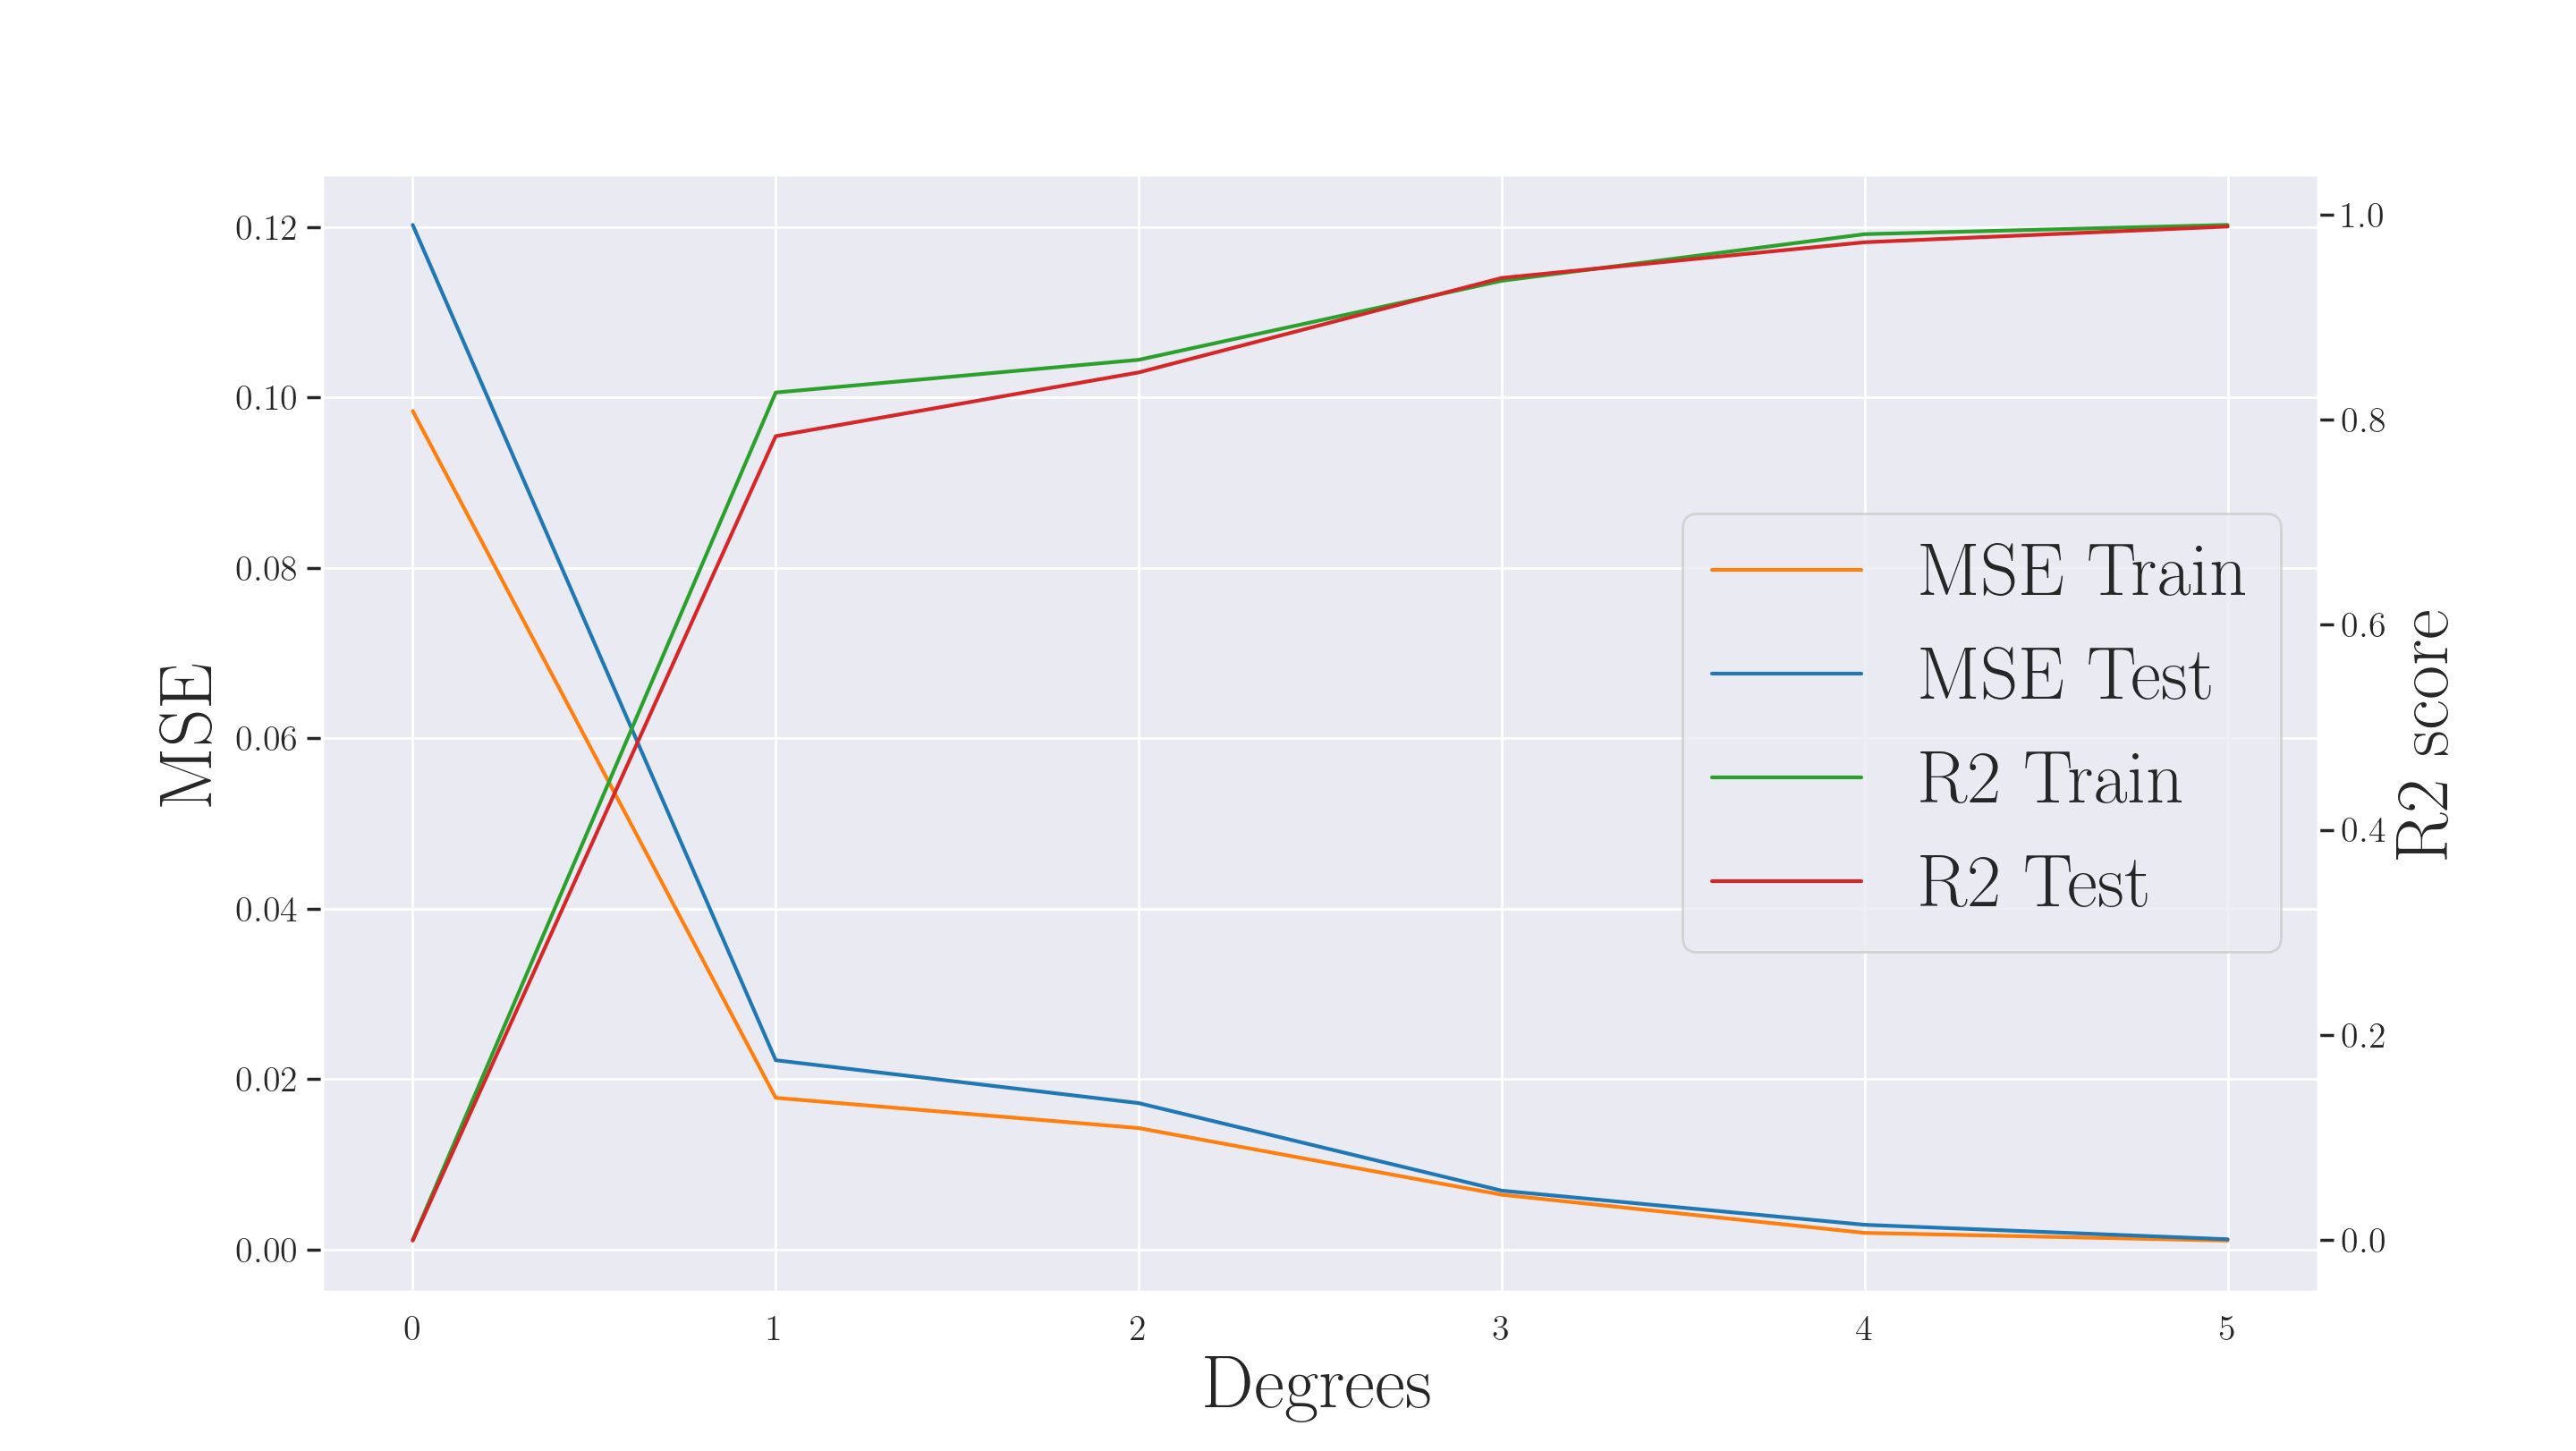
\includegraphics[width=\linewidth]{images/Figure_3.png}
	\caption{Plot showing the MSE and R2 score for the Franke function without noise. The regression method used was OLS.}
	\label{MSE and R2 OLS}
\end{figure}
\noindent The next step was to include noise given by the normal distribution $\mathcal{N}(0,0.1)$. Figure \eqref{MSE and R2 OLS noise} shows how the MSE and R2 score changes when noise is included in to the data set.
\begin{figure}[H]
	\centering
	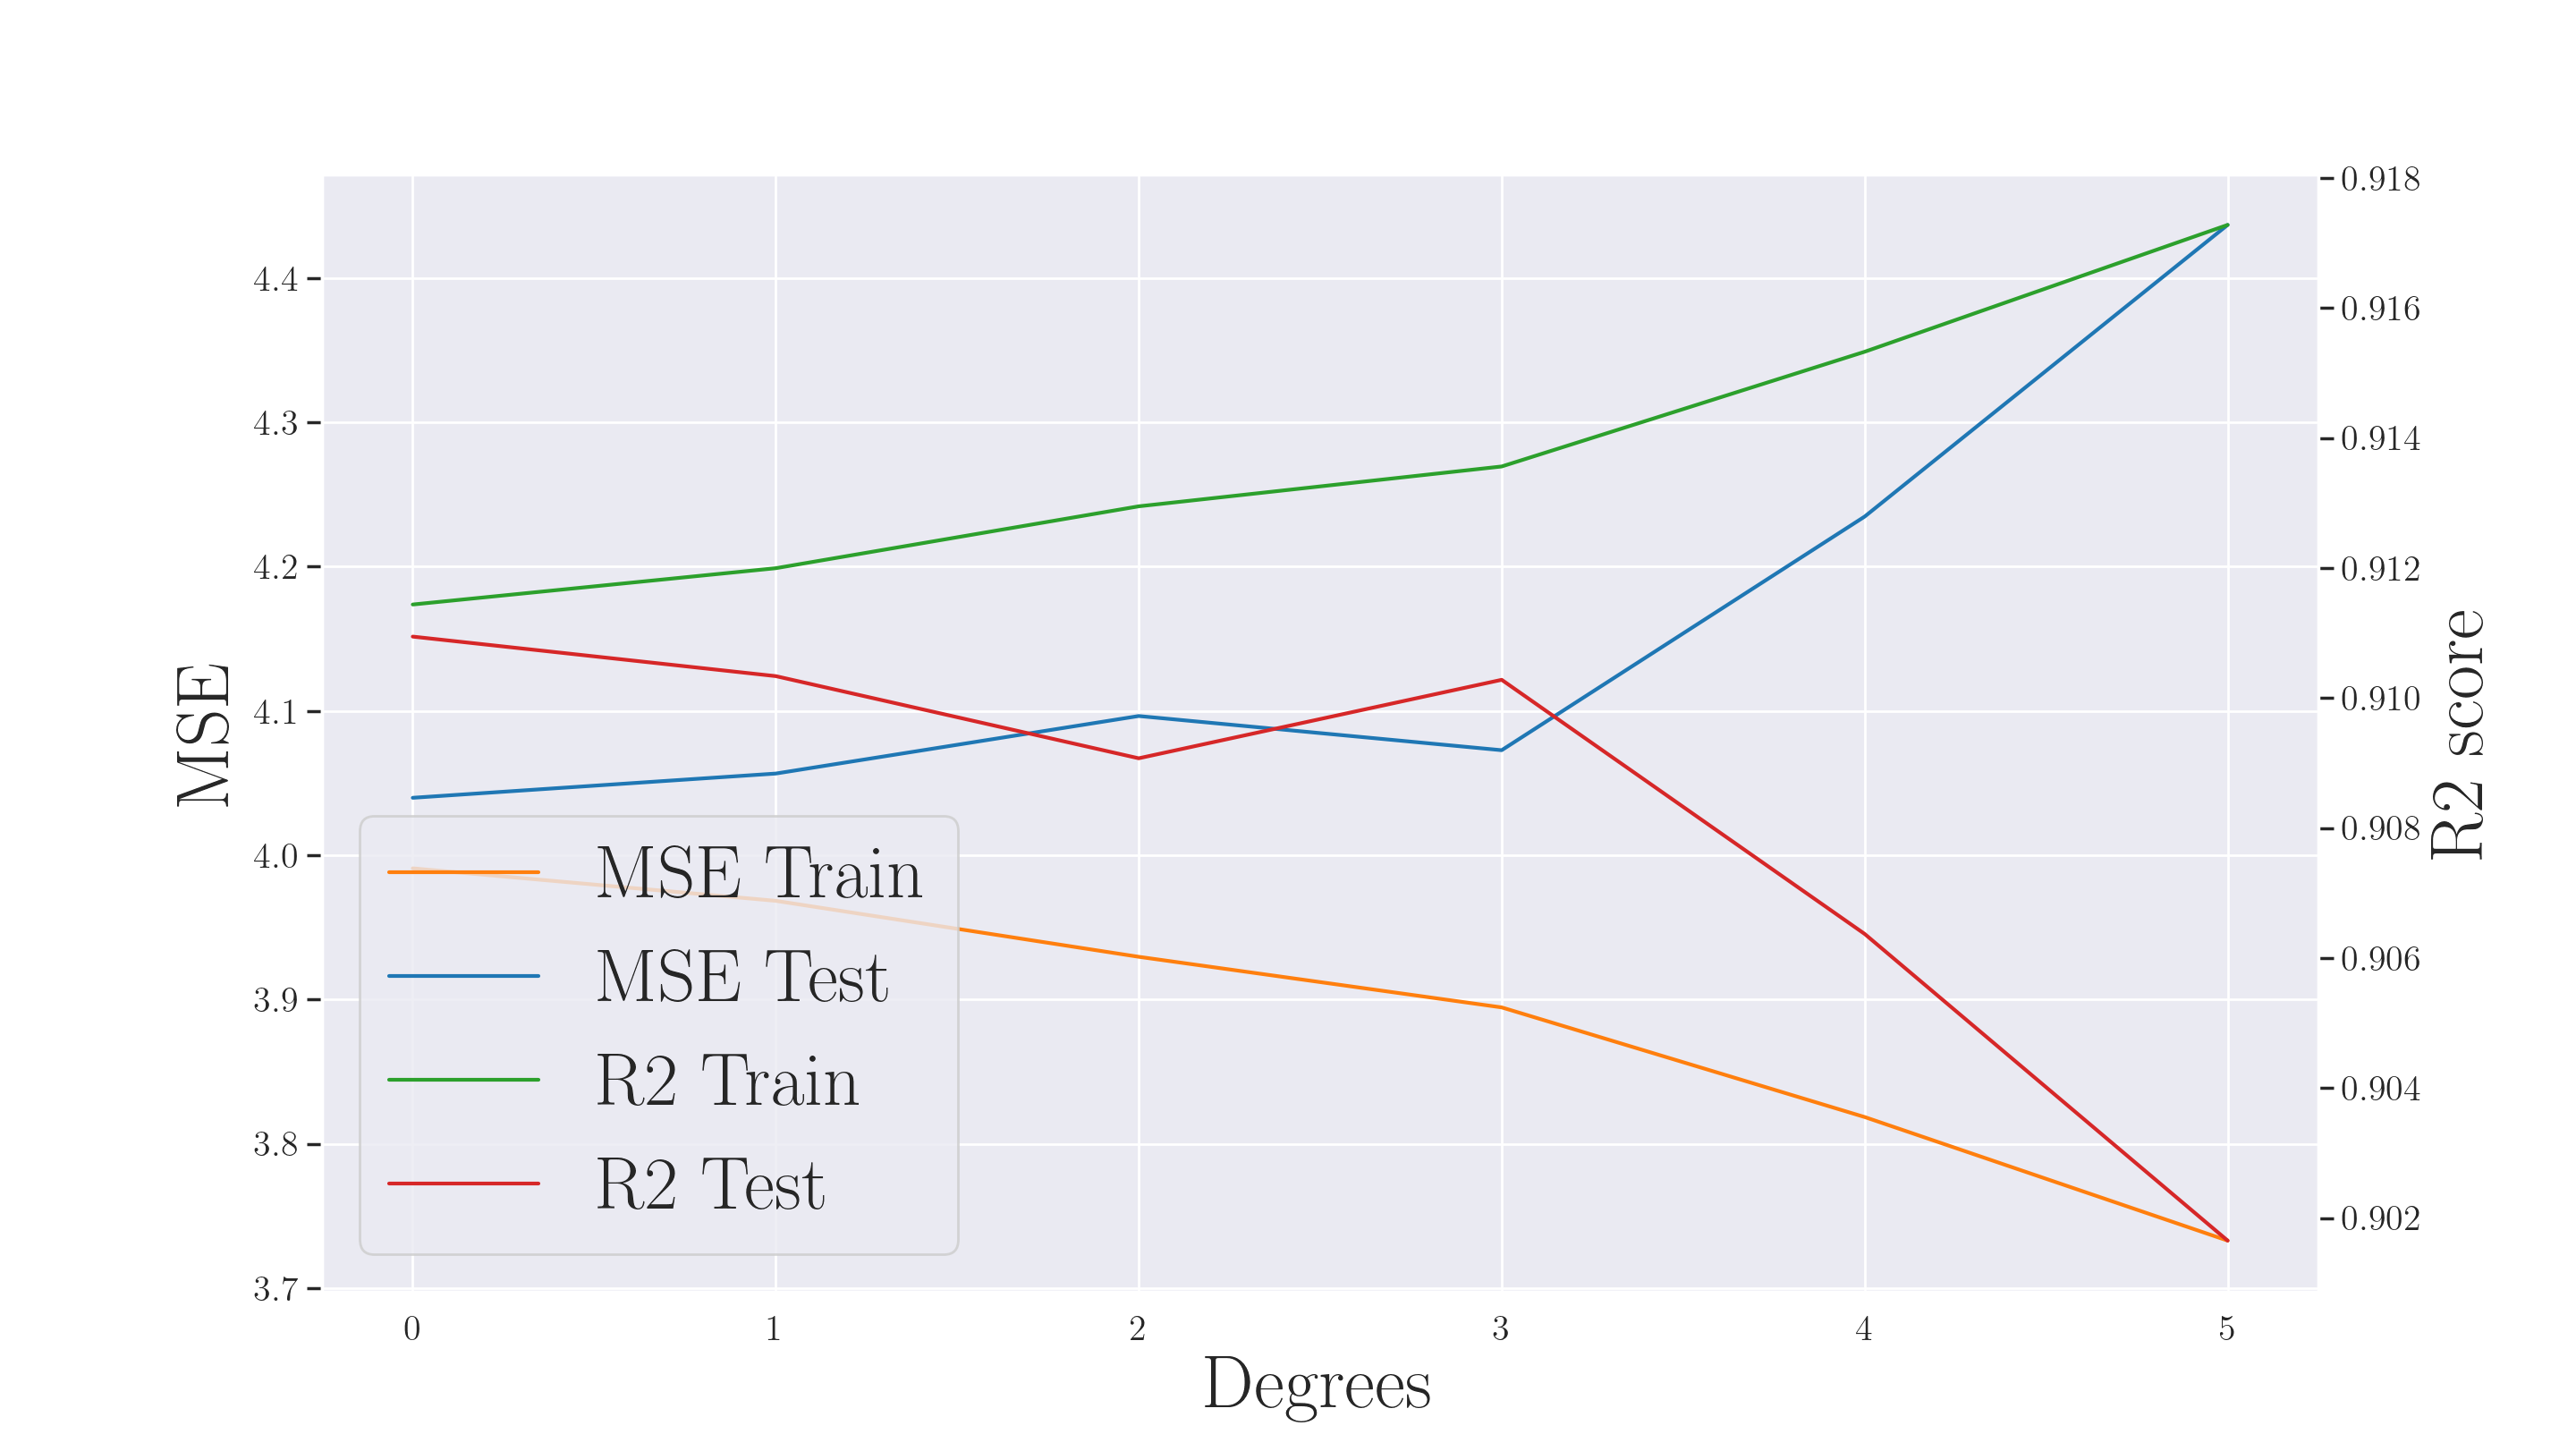
\includegraphics[width=\linewidth]{images/Figure_4.png}
	\caption{Plot showing the MSE and R2 score for the Franke function with noise $\mathcal{N}(0,0.1)$. The regression method used was OLS.}
	\label{MSE and R2 OLS noise}
\end{figure}
\noindent We then plotted the coefficients for the different orders of polynomials to see how these varies in value.
\begin{figure}[H]
	\centering
	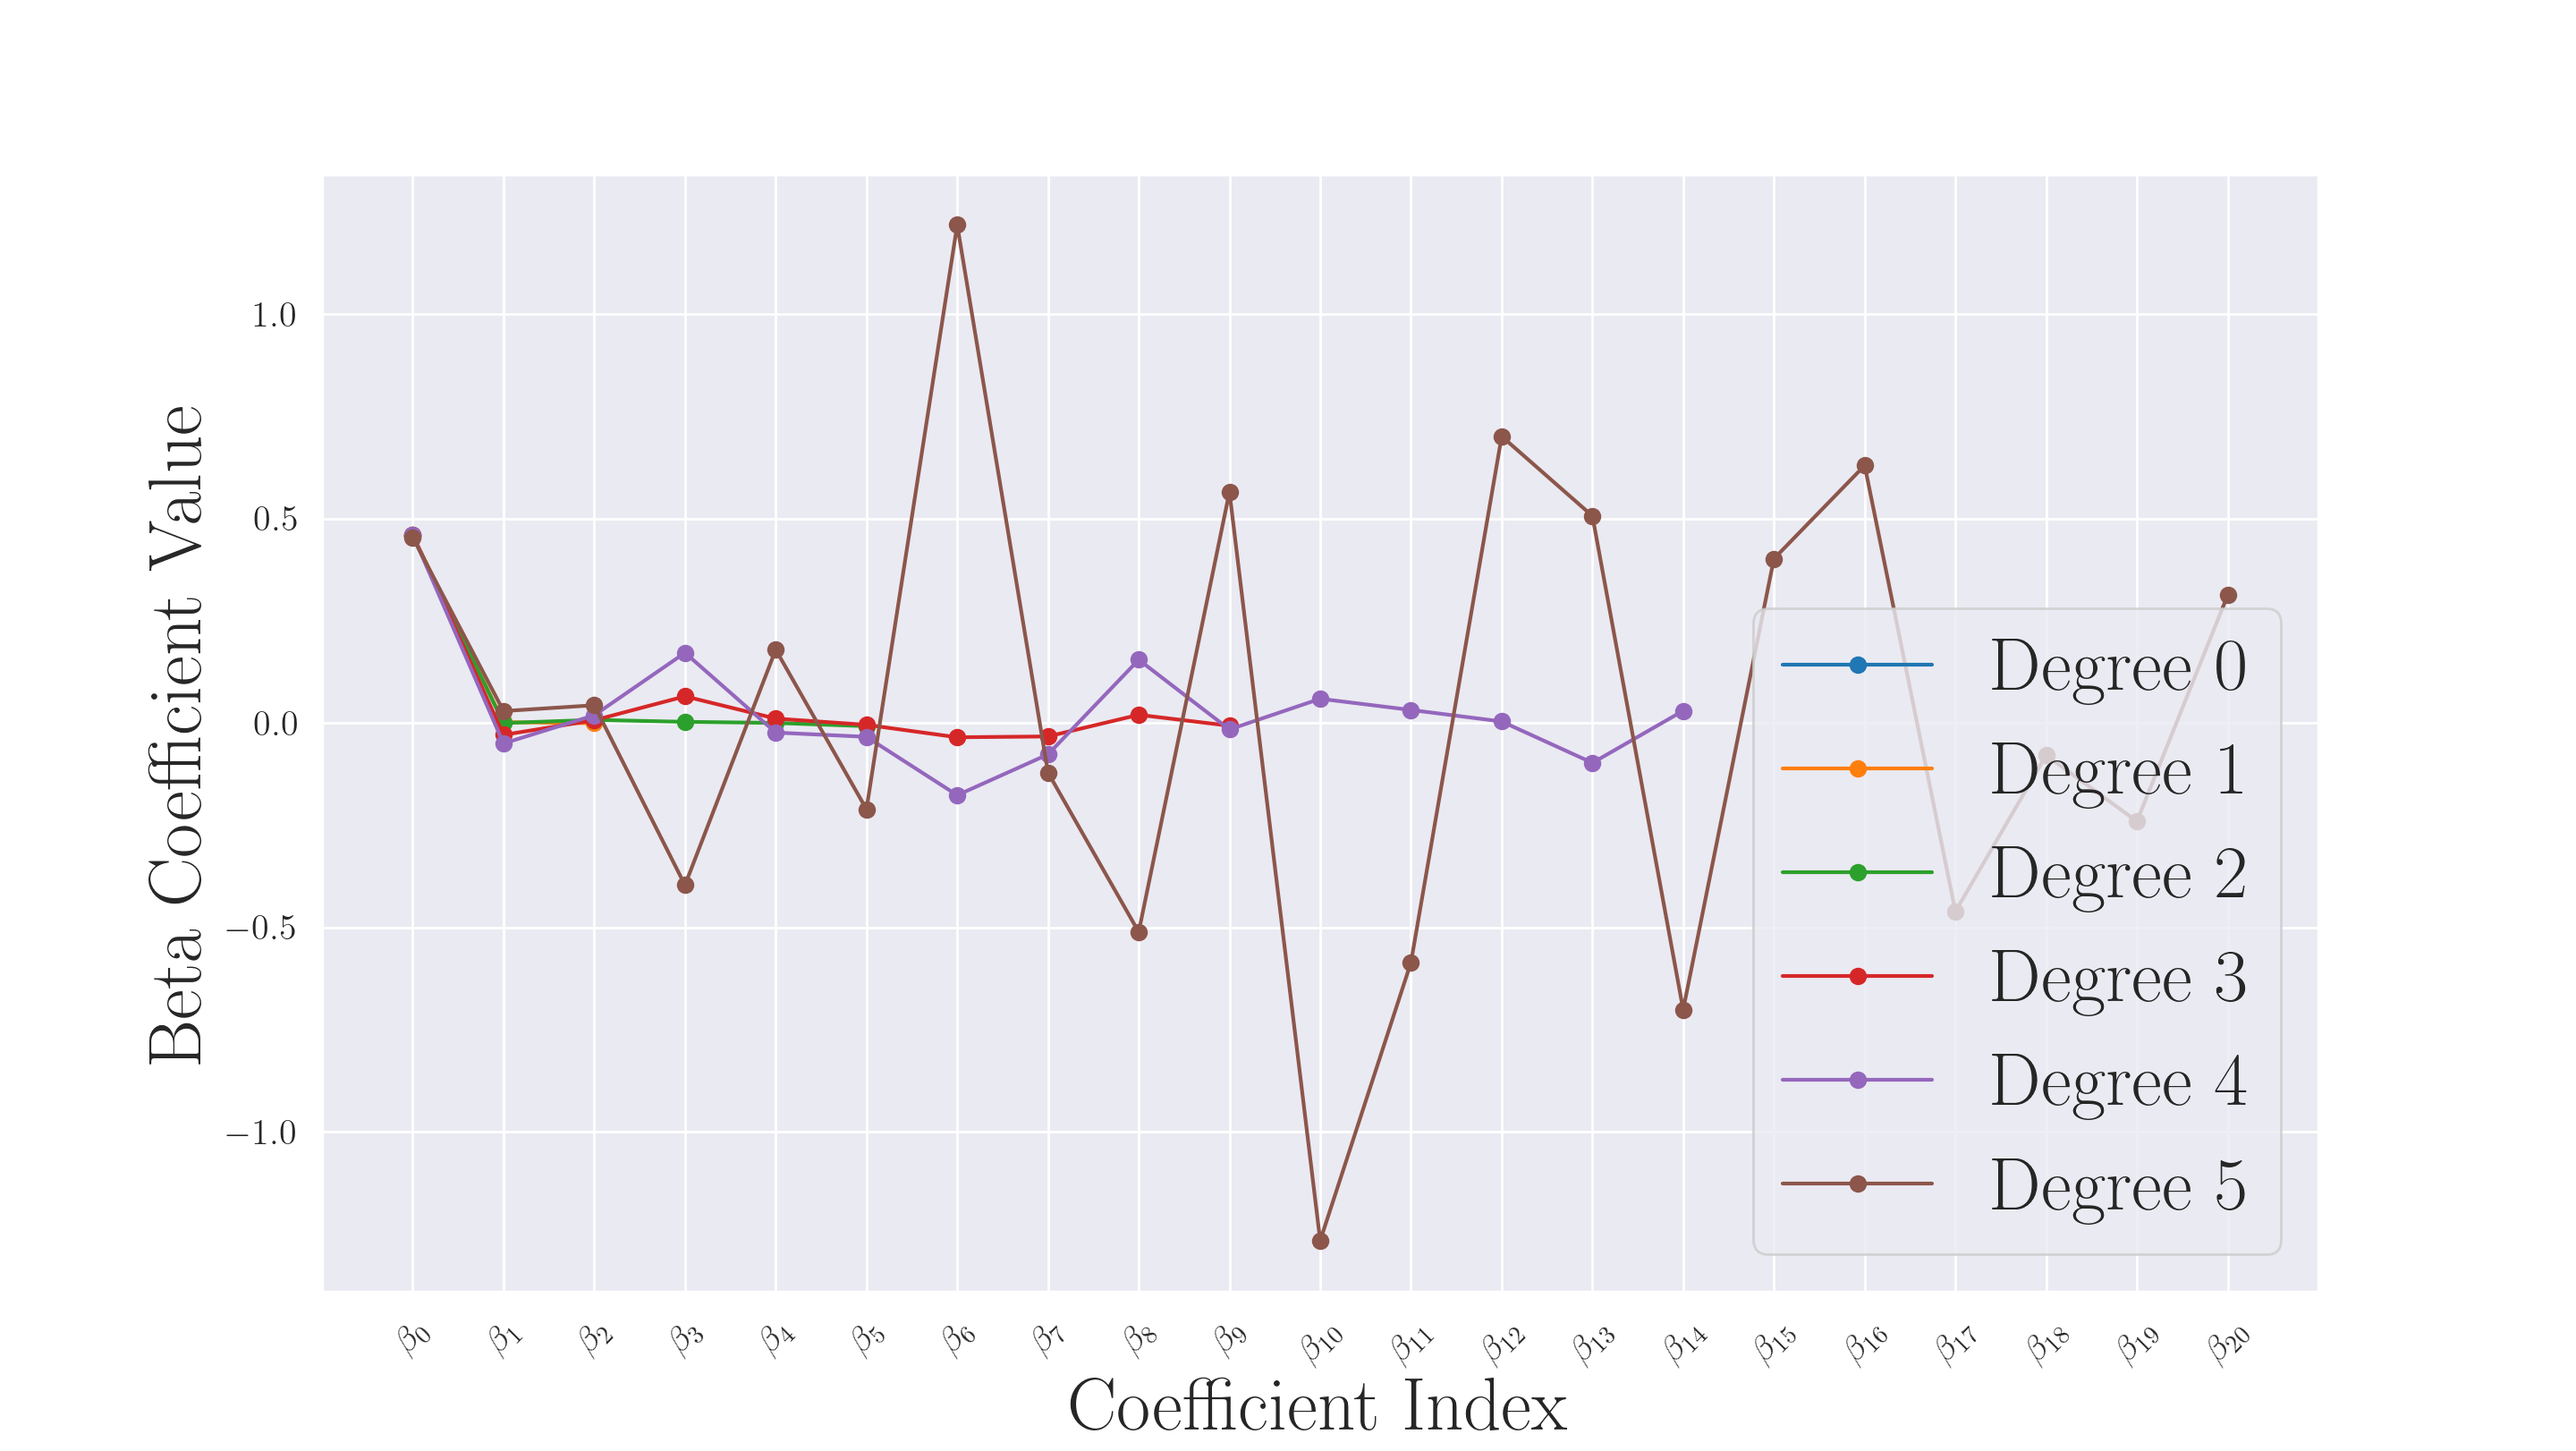
\includegraphics[width=\linewidth]{images/Figure_12.png}
	\caption{A plot showing the $\beta$ values for OLS for different orders of polynomials.}
	\label{beta OLS}
\end{figure}
%
\noindent Figure \ref{fig:bootstrap_error} is showing the error of training and test data for polynomial degree $0-15$. There is a consistent reduction in error of training for higher polynomial degree, whereas the error of test increase with polynomial degree $6-15$.
\begin{figure}[H]
	\centering
	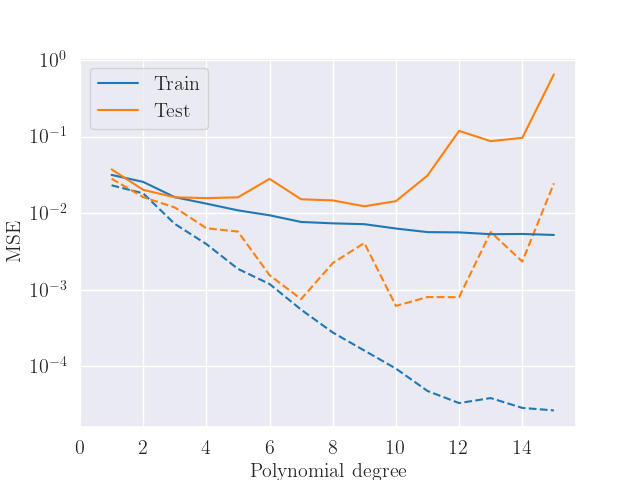
\includegraphics[width=\linewidth]{images/bootstrap_error.png}
	\caption{MSE of the models prediction for polynomial degree $0-15$, using the Franke function. The solid lines describe the MSE where noise is added to the function, dotted lines describe MSE where noise is not added.}
    \label{fig:bootstrap_error}
\end{figure}
%
\noindent Figure \ref{fig:bias_variance} is showing the error of prediction, and the bias and variance of the model for polynomial degree $0-15$. 
% 
\begin{figure}[H]
    \centering
    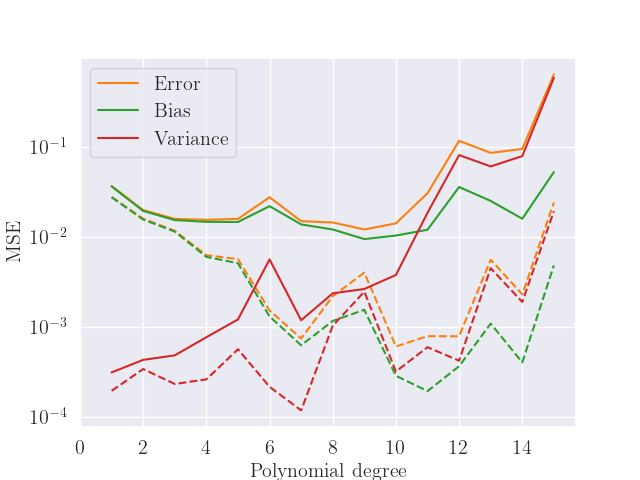
\includegraphics[width=\linewidth]{images/bias_variance.png}
    \caption{MSE of the models predicted error, using the Franke function, bias and variance. The solid lines describe the MSE where noise is added to the function, dotted lines describe MSE where noise is not added.}
    \label{fig:bias_variance}
\end{figure}
\noindent We compared number of folds used when re-sampling data from the Franke funktion without noise, by using OLS as regression method. In figure \ref{fig:cv_kfolds} we plot MSE for each fold $k=[5-10]$, to determine an ideal division of the data available.
\begin{figure}[H]
	\centering
	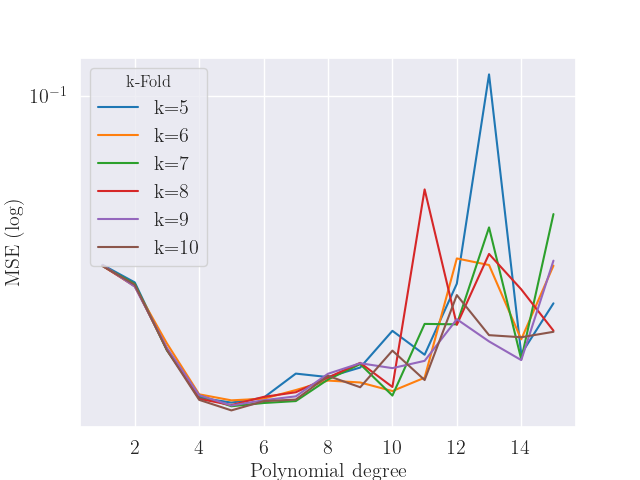
\includegraphics[width=\linewidth]{images/cv_kfolds.png}
	\caption{MSE of prediction error for polynomial degree $0-15$, using the Franke function, with cross validation $k=5-10$.}
 \label{fig:cv_kfolds}
\end{figure}

\subsubsection{Ridge}
\noindent For Ridge regression we started by making a heat map of how the MSE changes as a function of complexity and $\lambda$ values. Here we tested for 1000 different $lambda$ values from $\lambda_0 = 10^{-8}$ to $\lambda_{1000} = 10^{2}$ and for polynomials with degree 1-5. A plot of the heat map for both the training and testing data set is shown in figure \eqref{heatmap training ridge} and \eqref{heatmap test ridge}.
\begin{figure}[h]
	\centering
	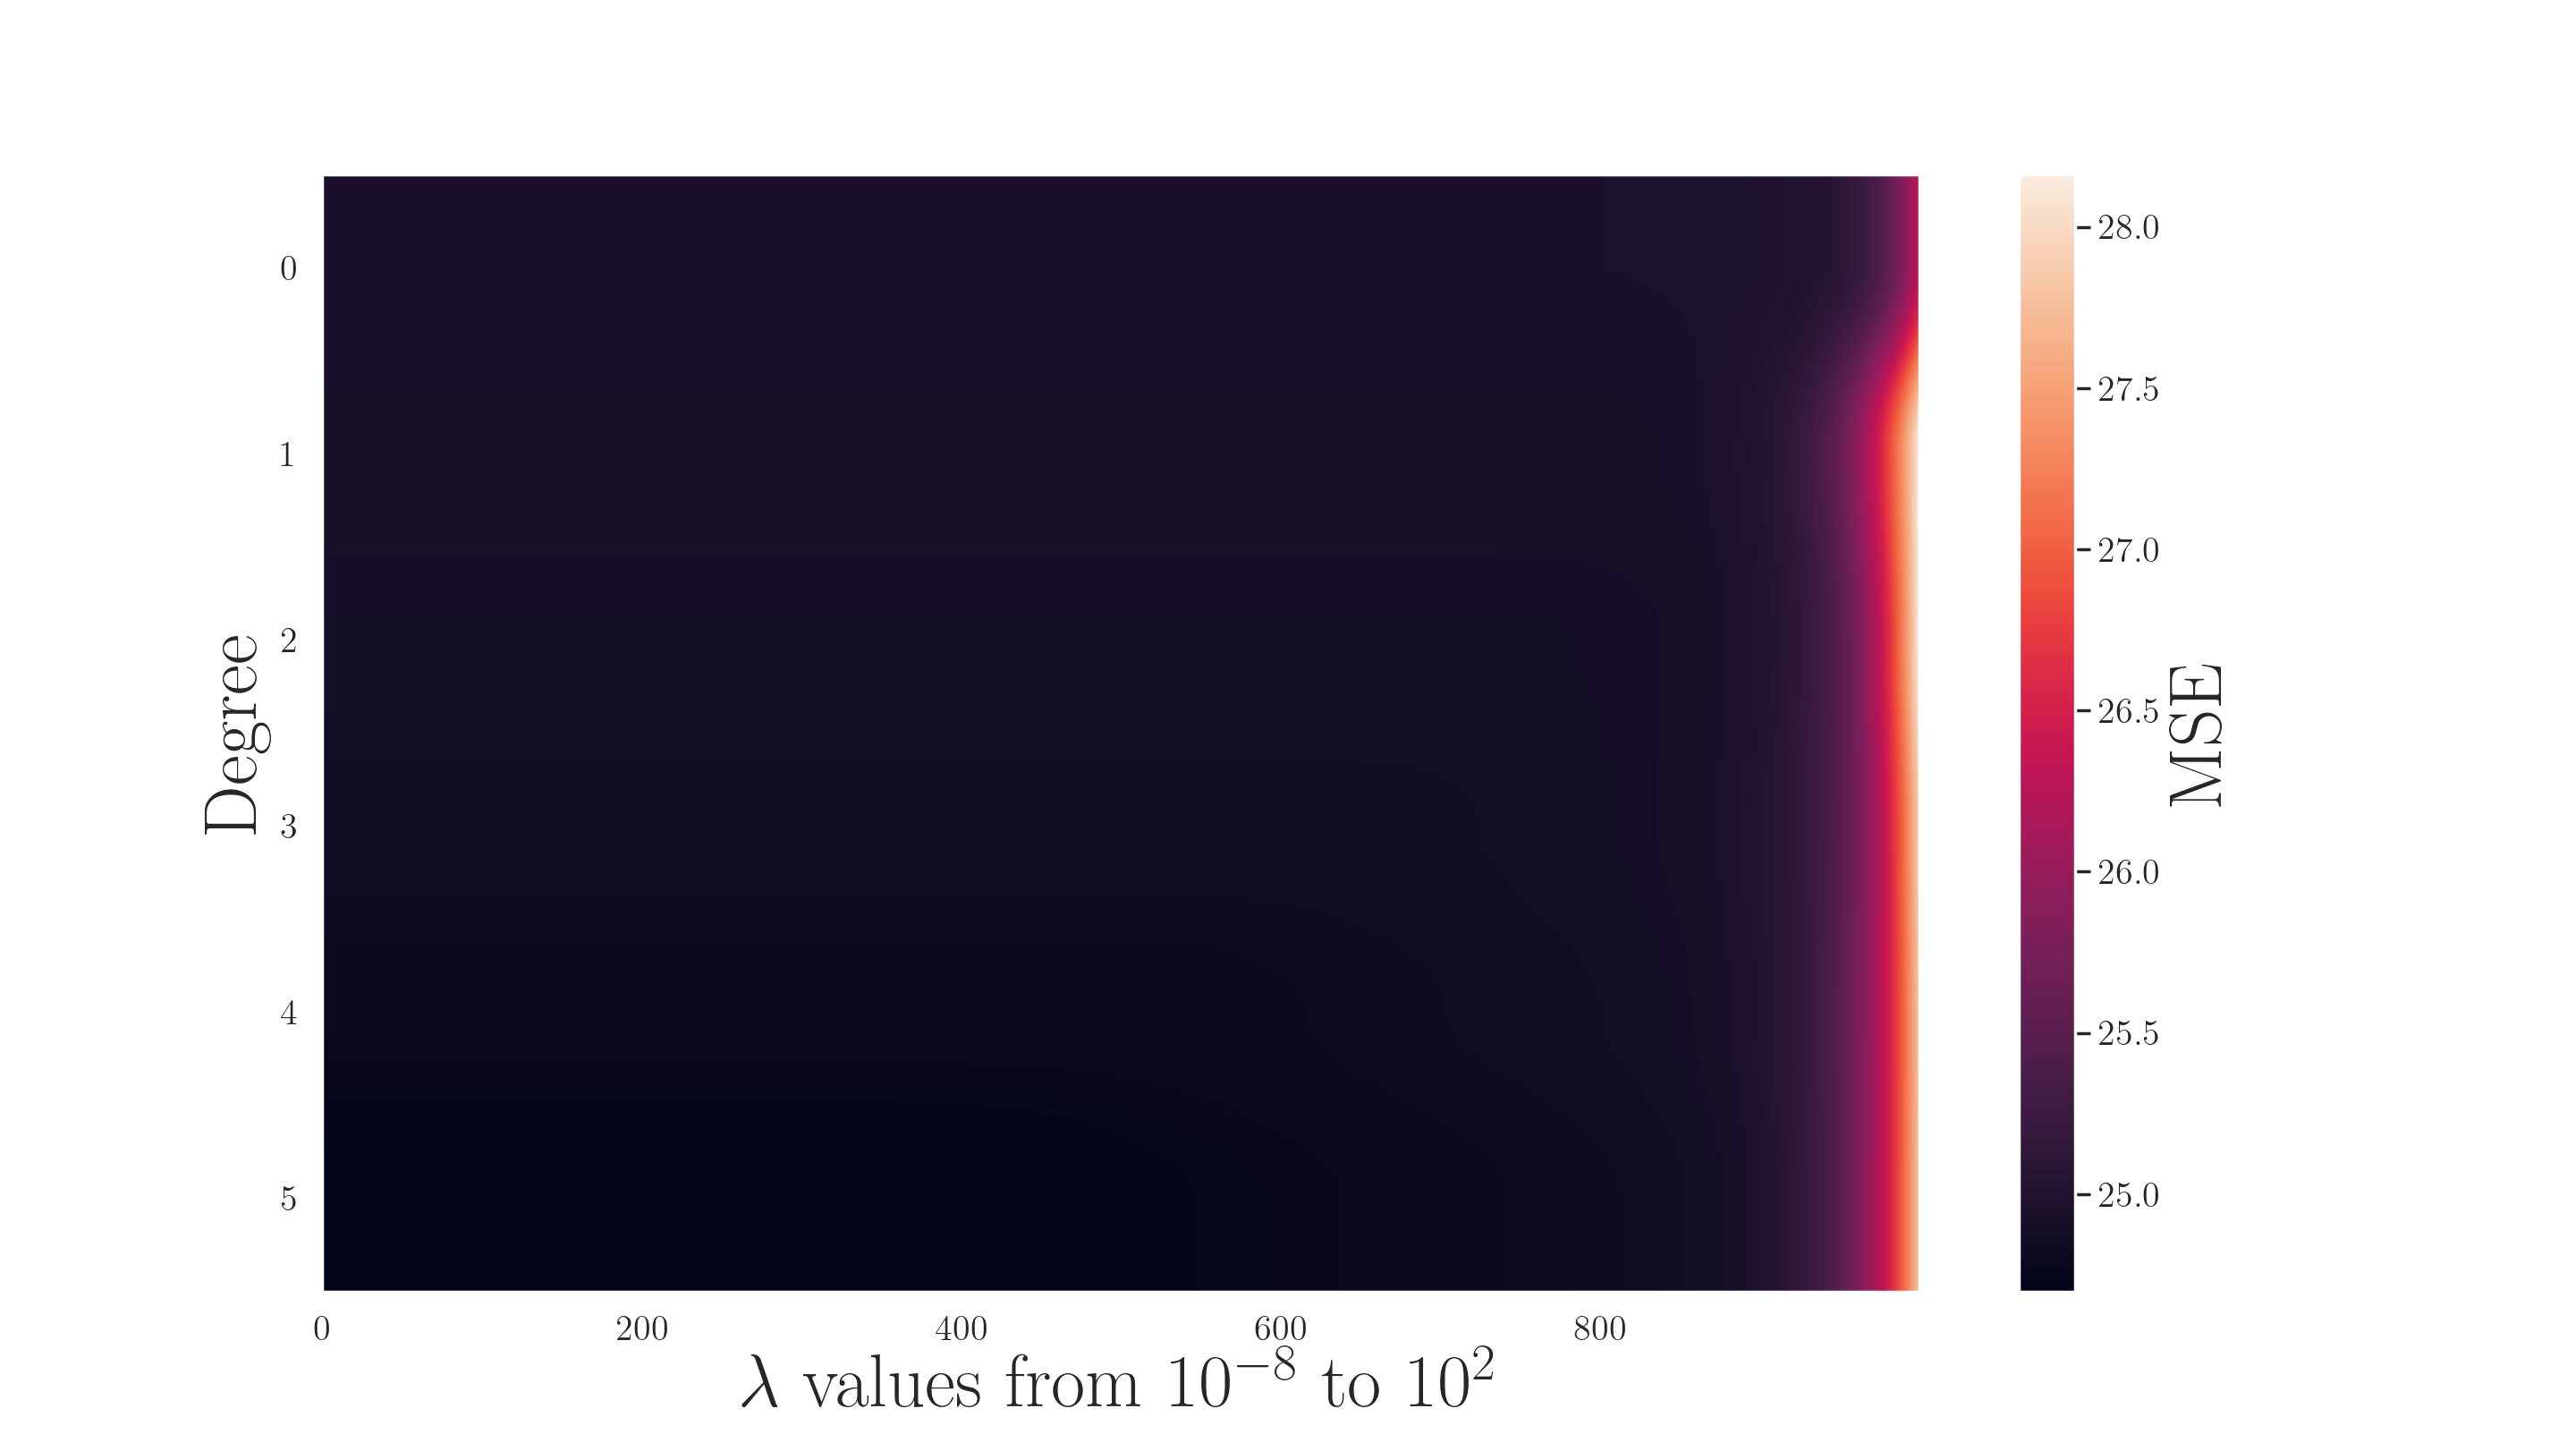
\includegraphics[width=\linewidth]{images/Figure_8.png}
	\caption{A heat map of the MSE for the training data, for different $\lambda$ values and complexities. The $\lambda$ values goes from $10^{-8}$ to $10^{2}$. }
	\label{heatmap training ridge}
\end{figure}
\begin{figure}[H]
	\centering
	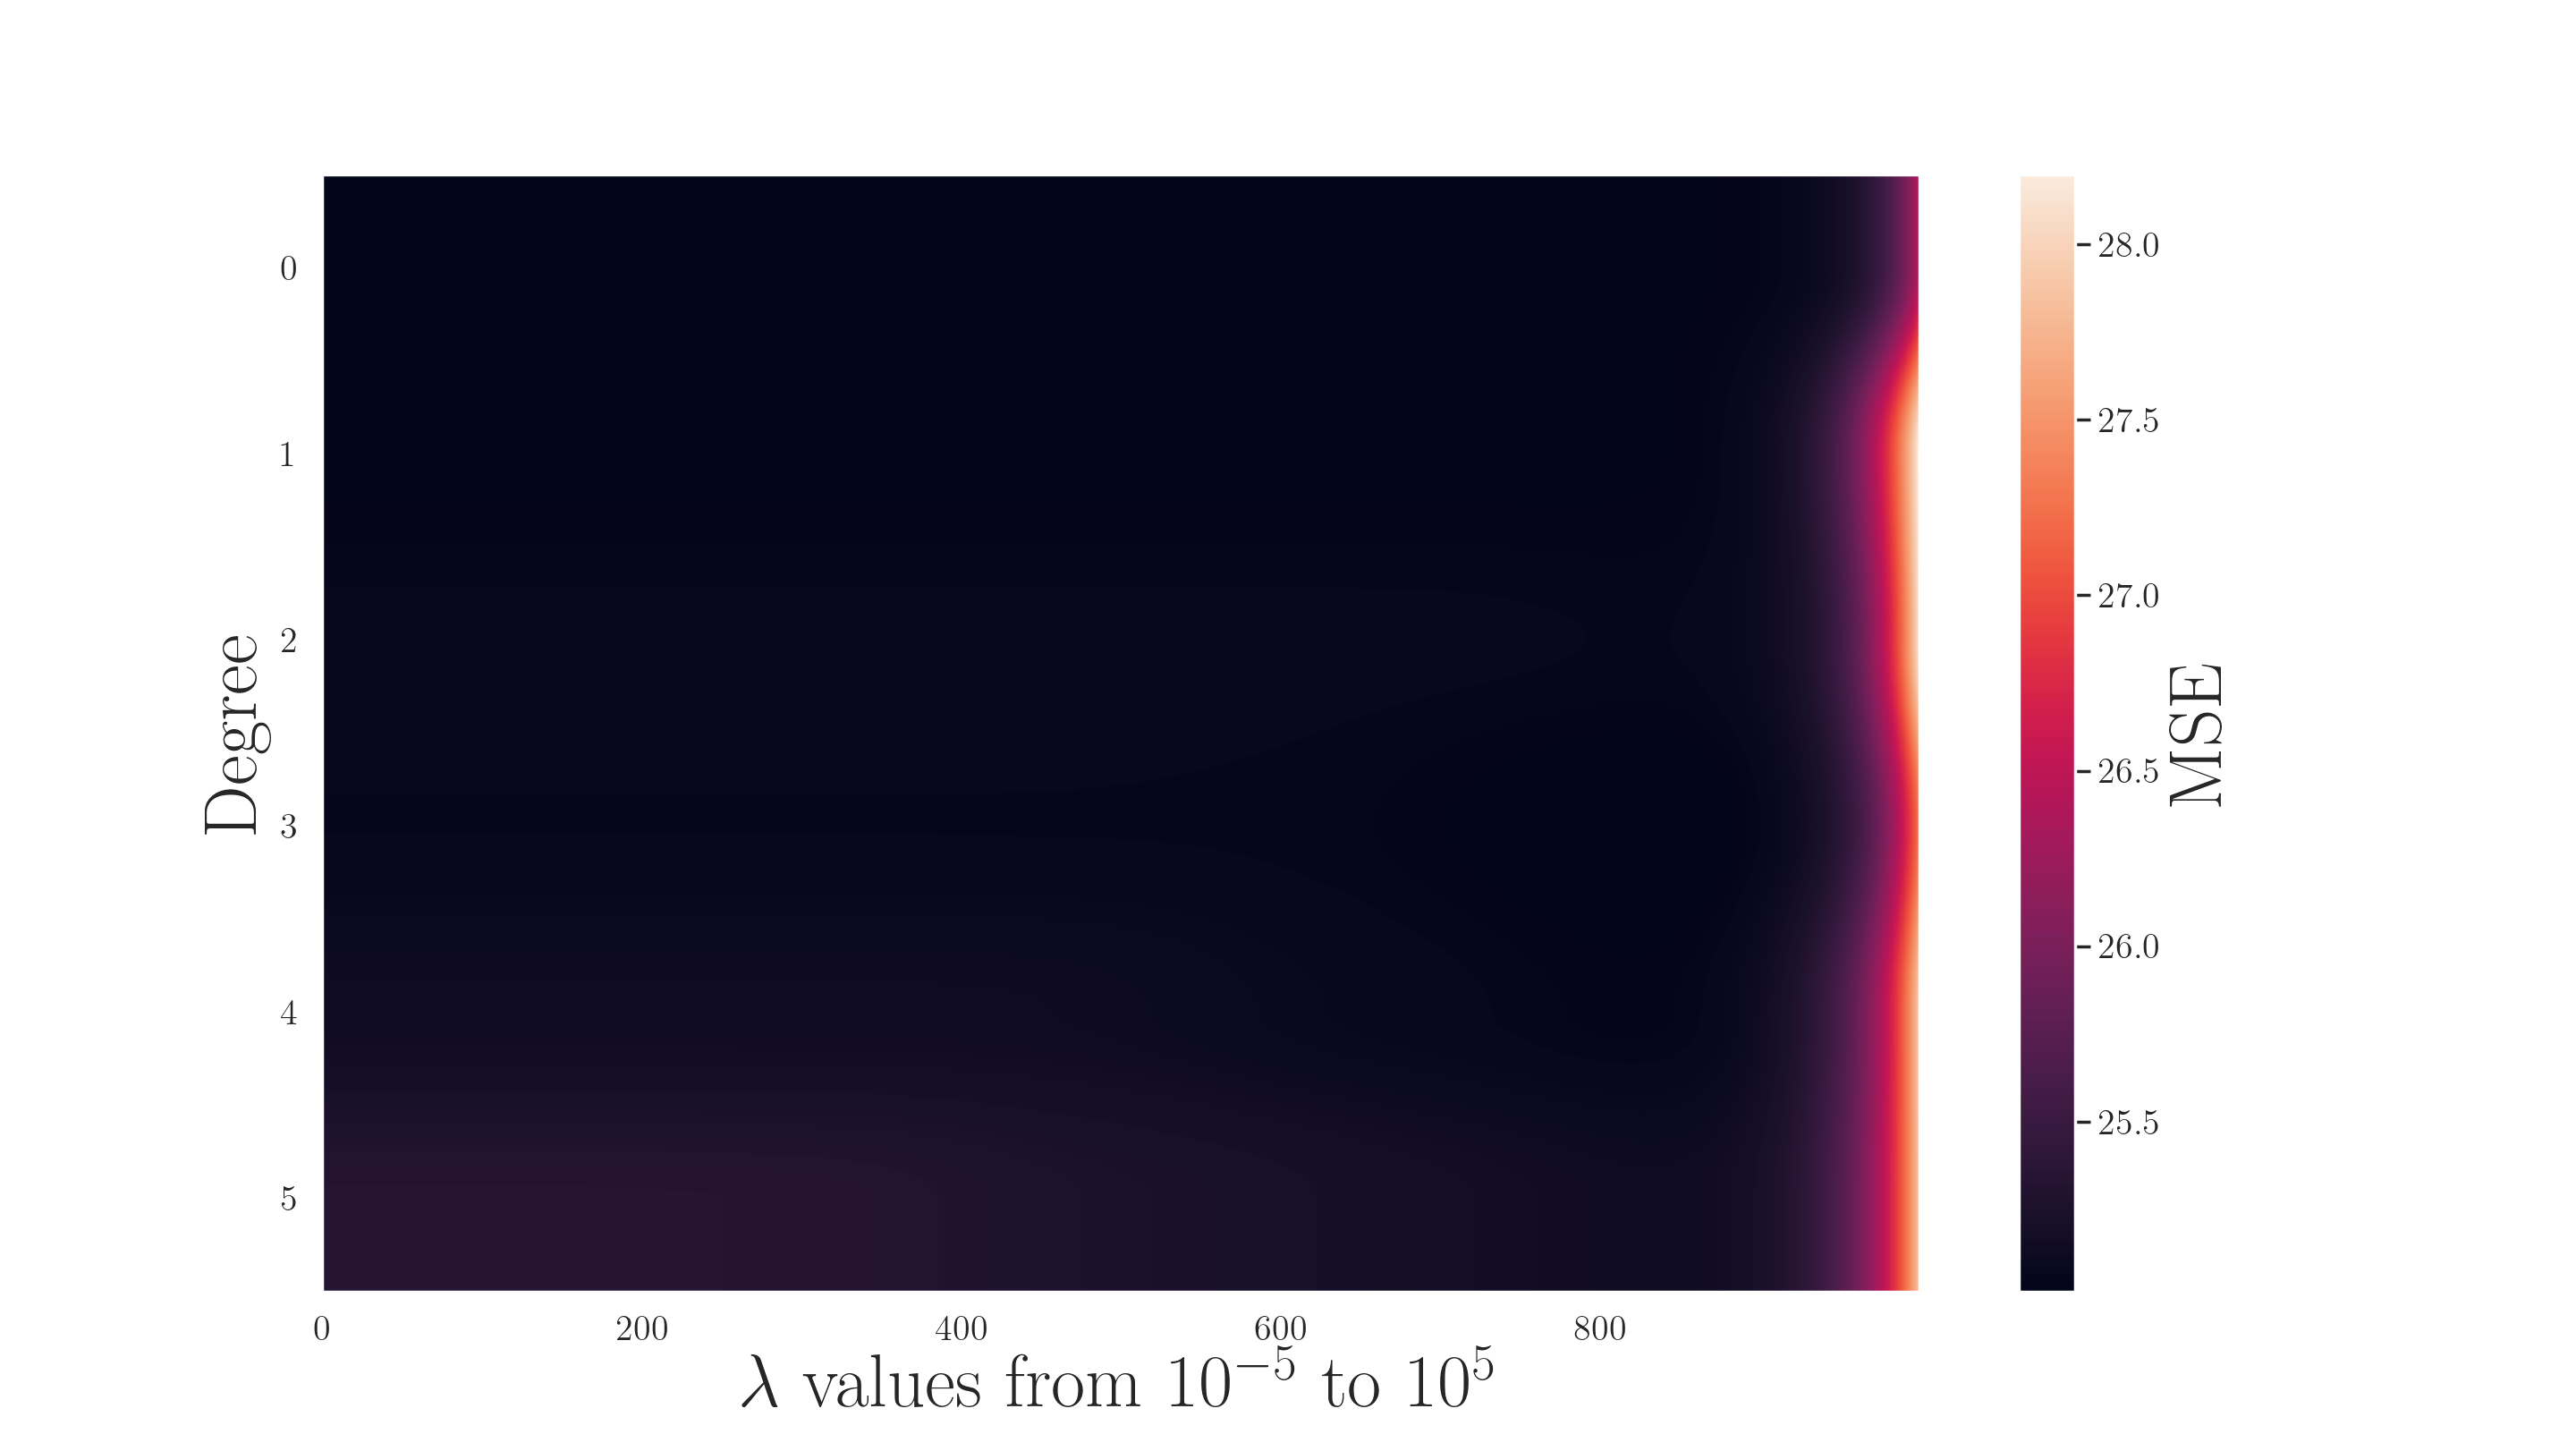
\includegraphics[width=\linewidth]{images/Figure_7.png}
	\caption{A heat map of the MSE for the testing data, for different $\lambda$ values and complexities. The $\lambda$ values goes from $10^{-5}$ to $10^{5}$.}
	\label{heatmap test ridge}
\end{figure}
\noindent Next we used the first $\lambda$ to plot how the MSE and R2 score changes as a function of complexity for the Franke function both with and without noise. Figure \eqref{MSE and R2 Ridge no noise} shows the MSE and R2 score with no noise present in the data set of the Franke function, and figure \eqref{MSE and R2 Ridge noise} shows with noise given by the normal distribution $\mathcal{N}(0,0.1)$.
\begin{figure}[H]
	\centering
	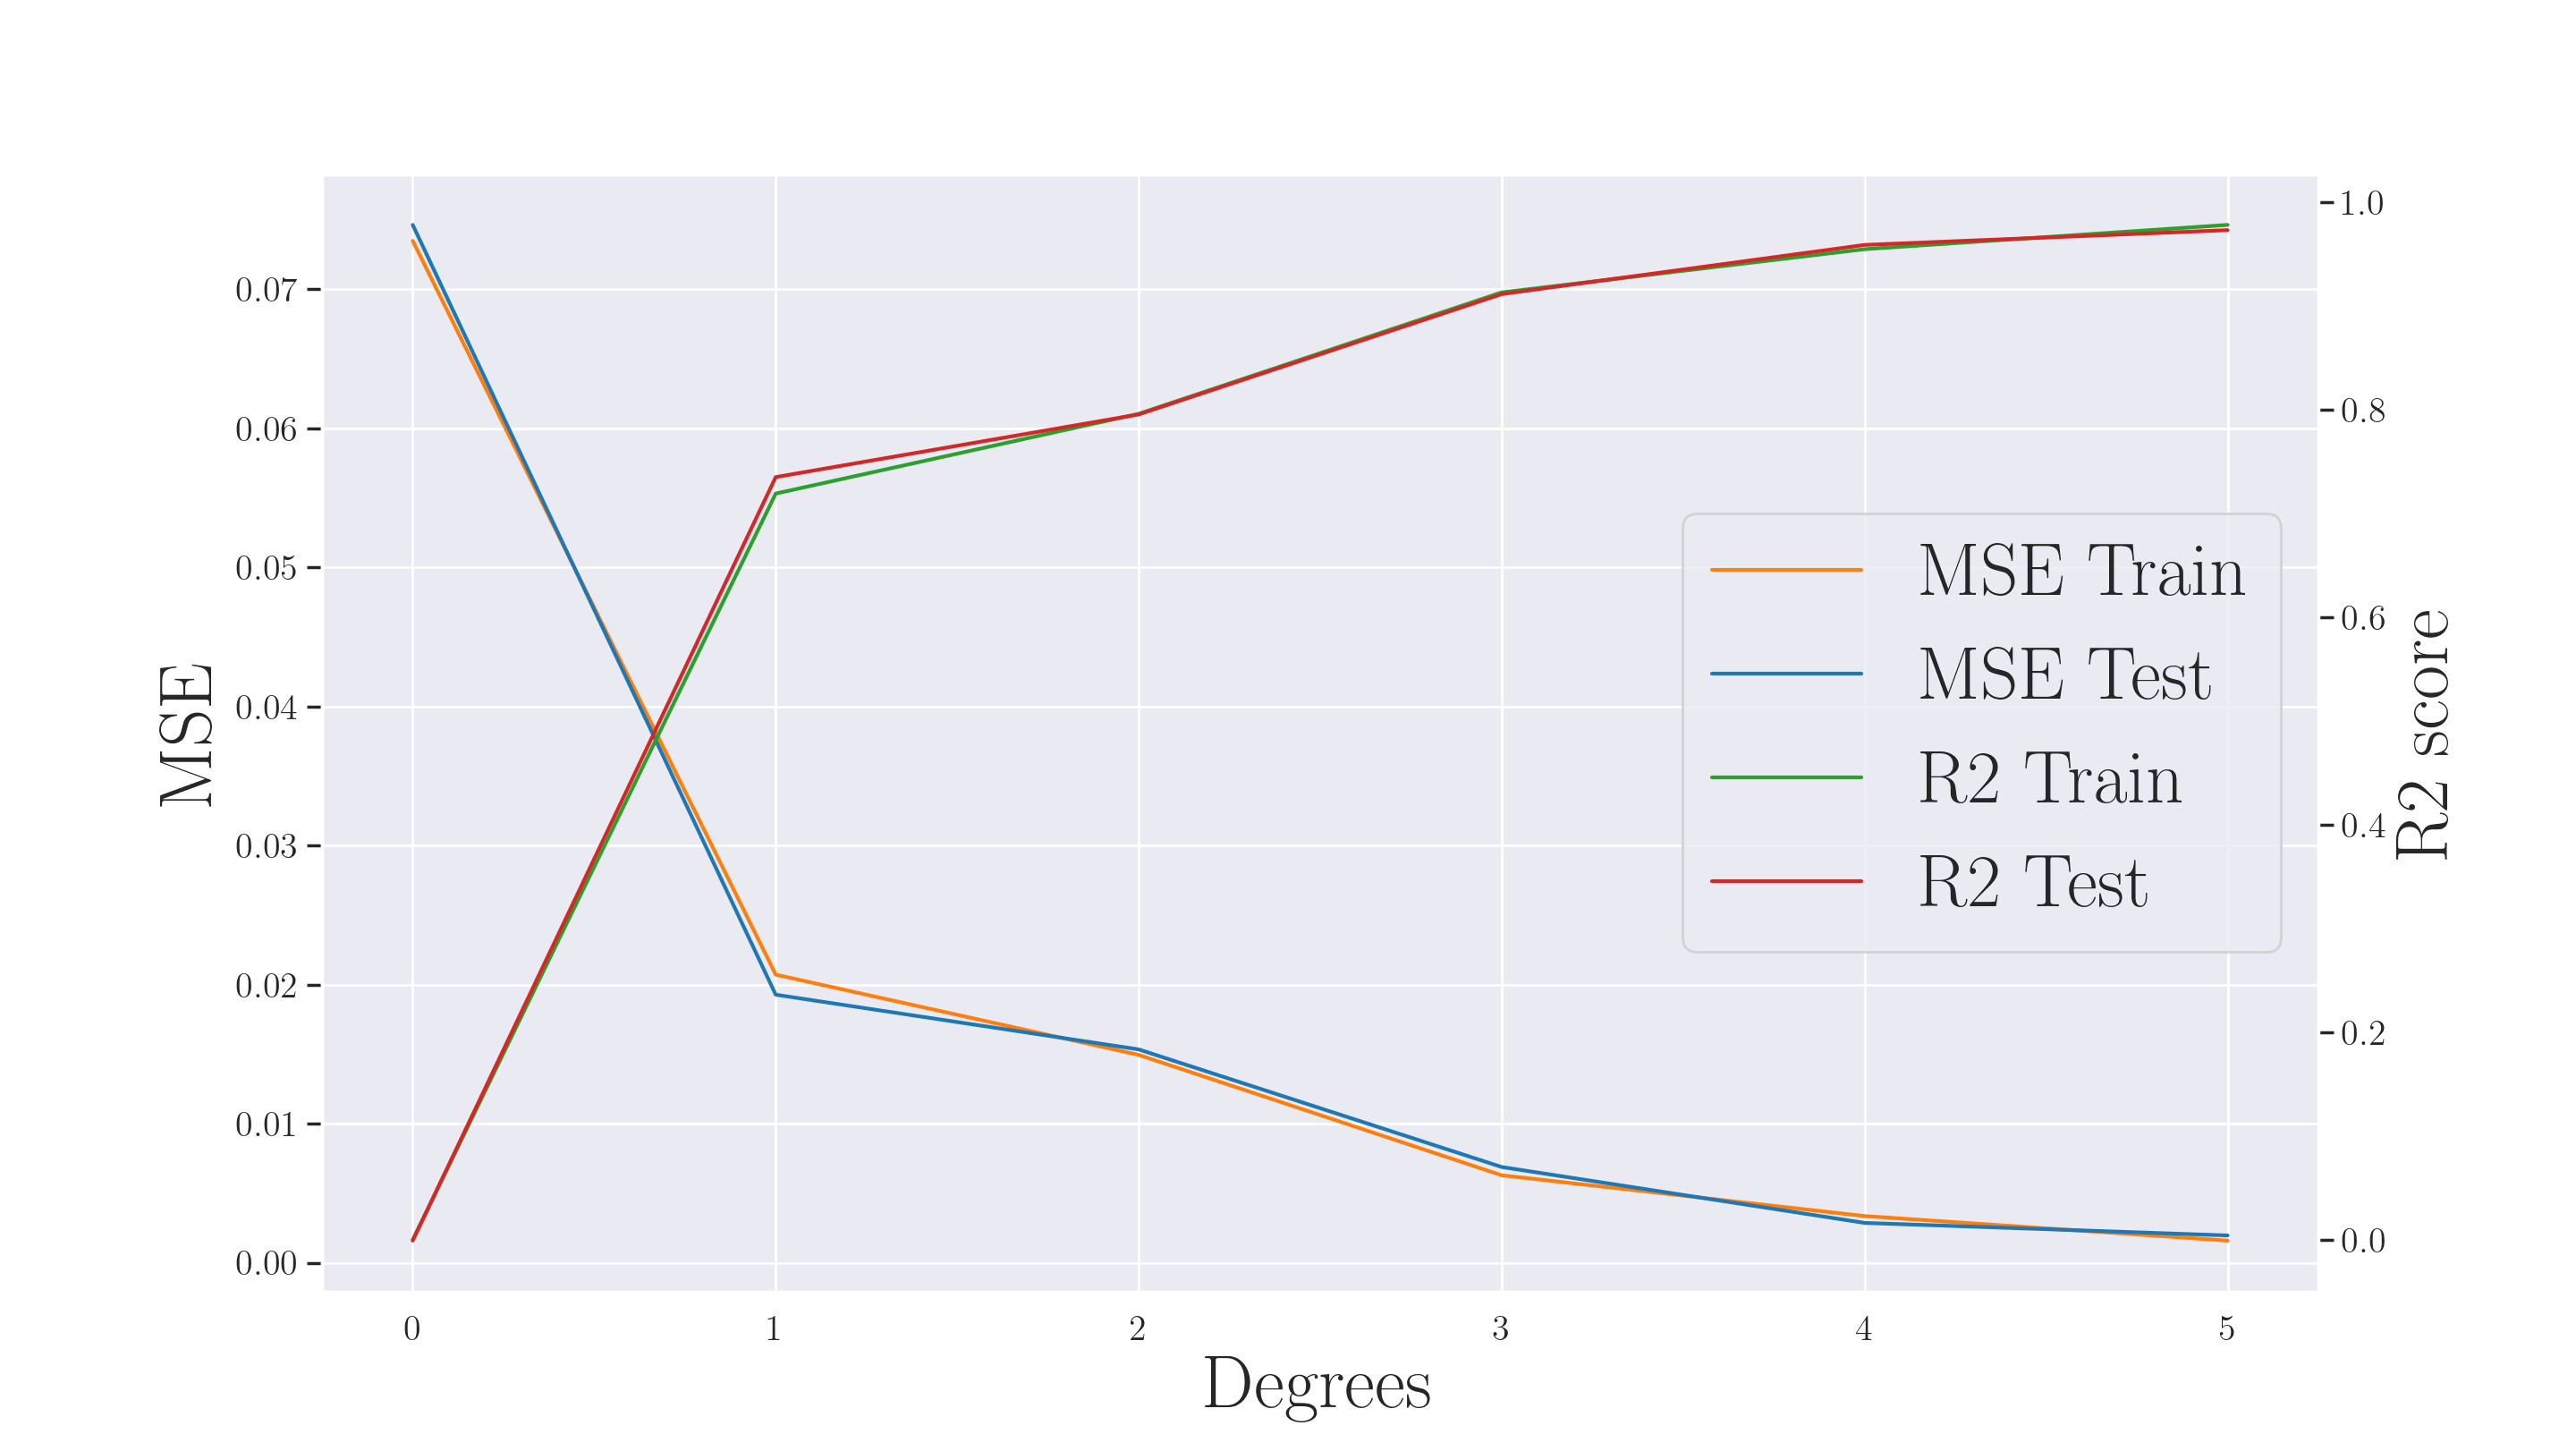
\includegraphics[width=\linewidth]{images/Figure_15.png}
	\caption{A plot of the MSE and R2 score as a function of degrees and a $\lambda$ value of $10^{-5}$ for Ridge regression on the Franke function with no noise present.}
	\label{MSE and R2 Ridge no noise}
\end{figure}
\begin{figure}[H]
	\centering
	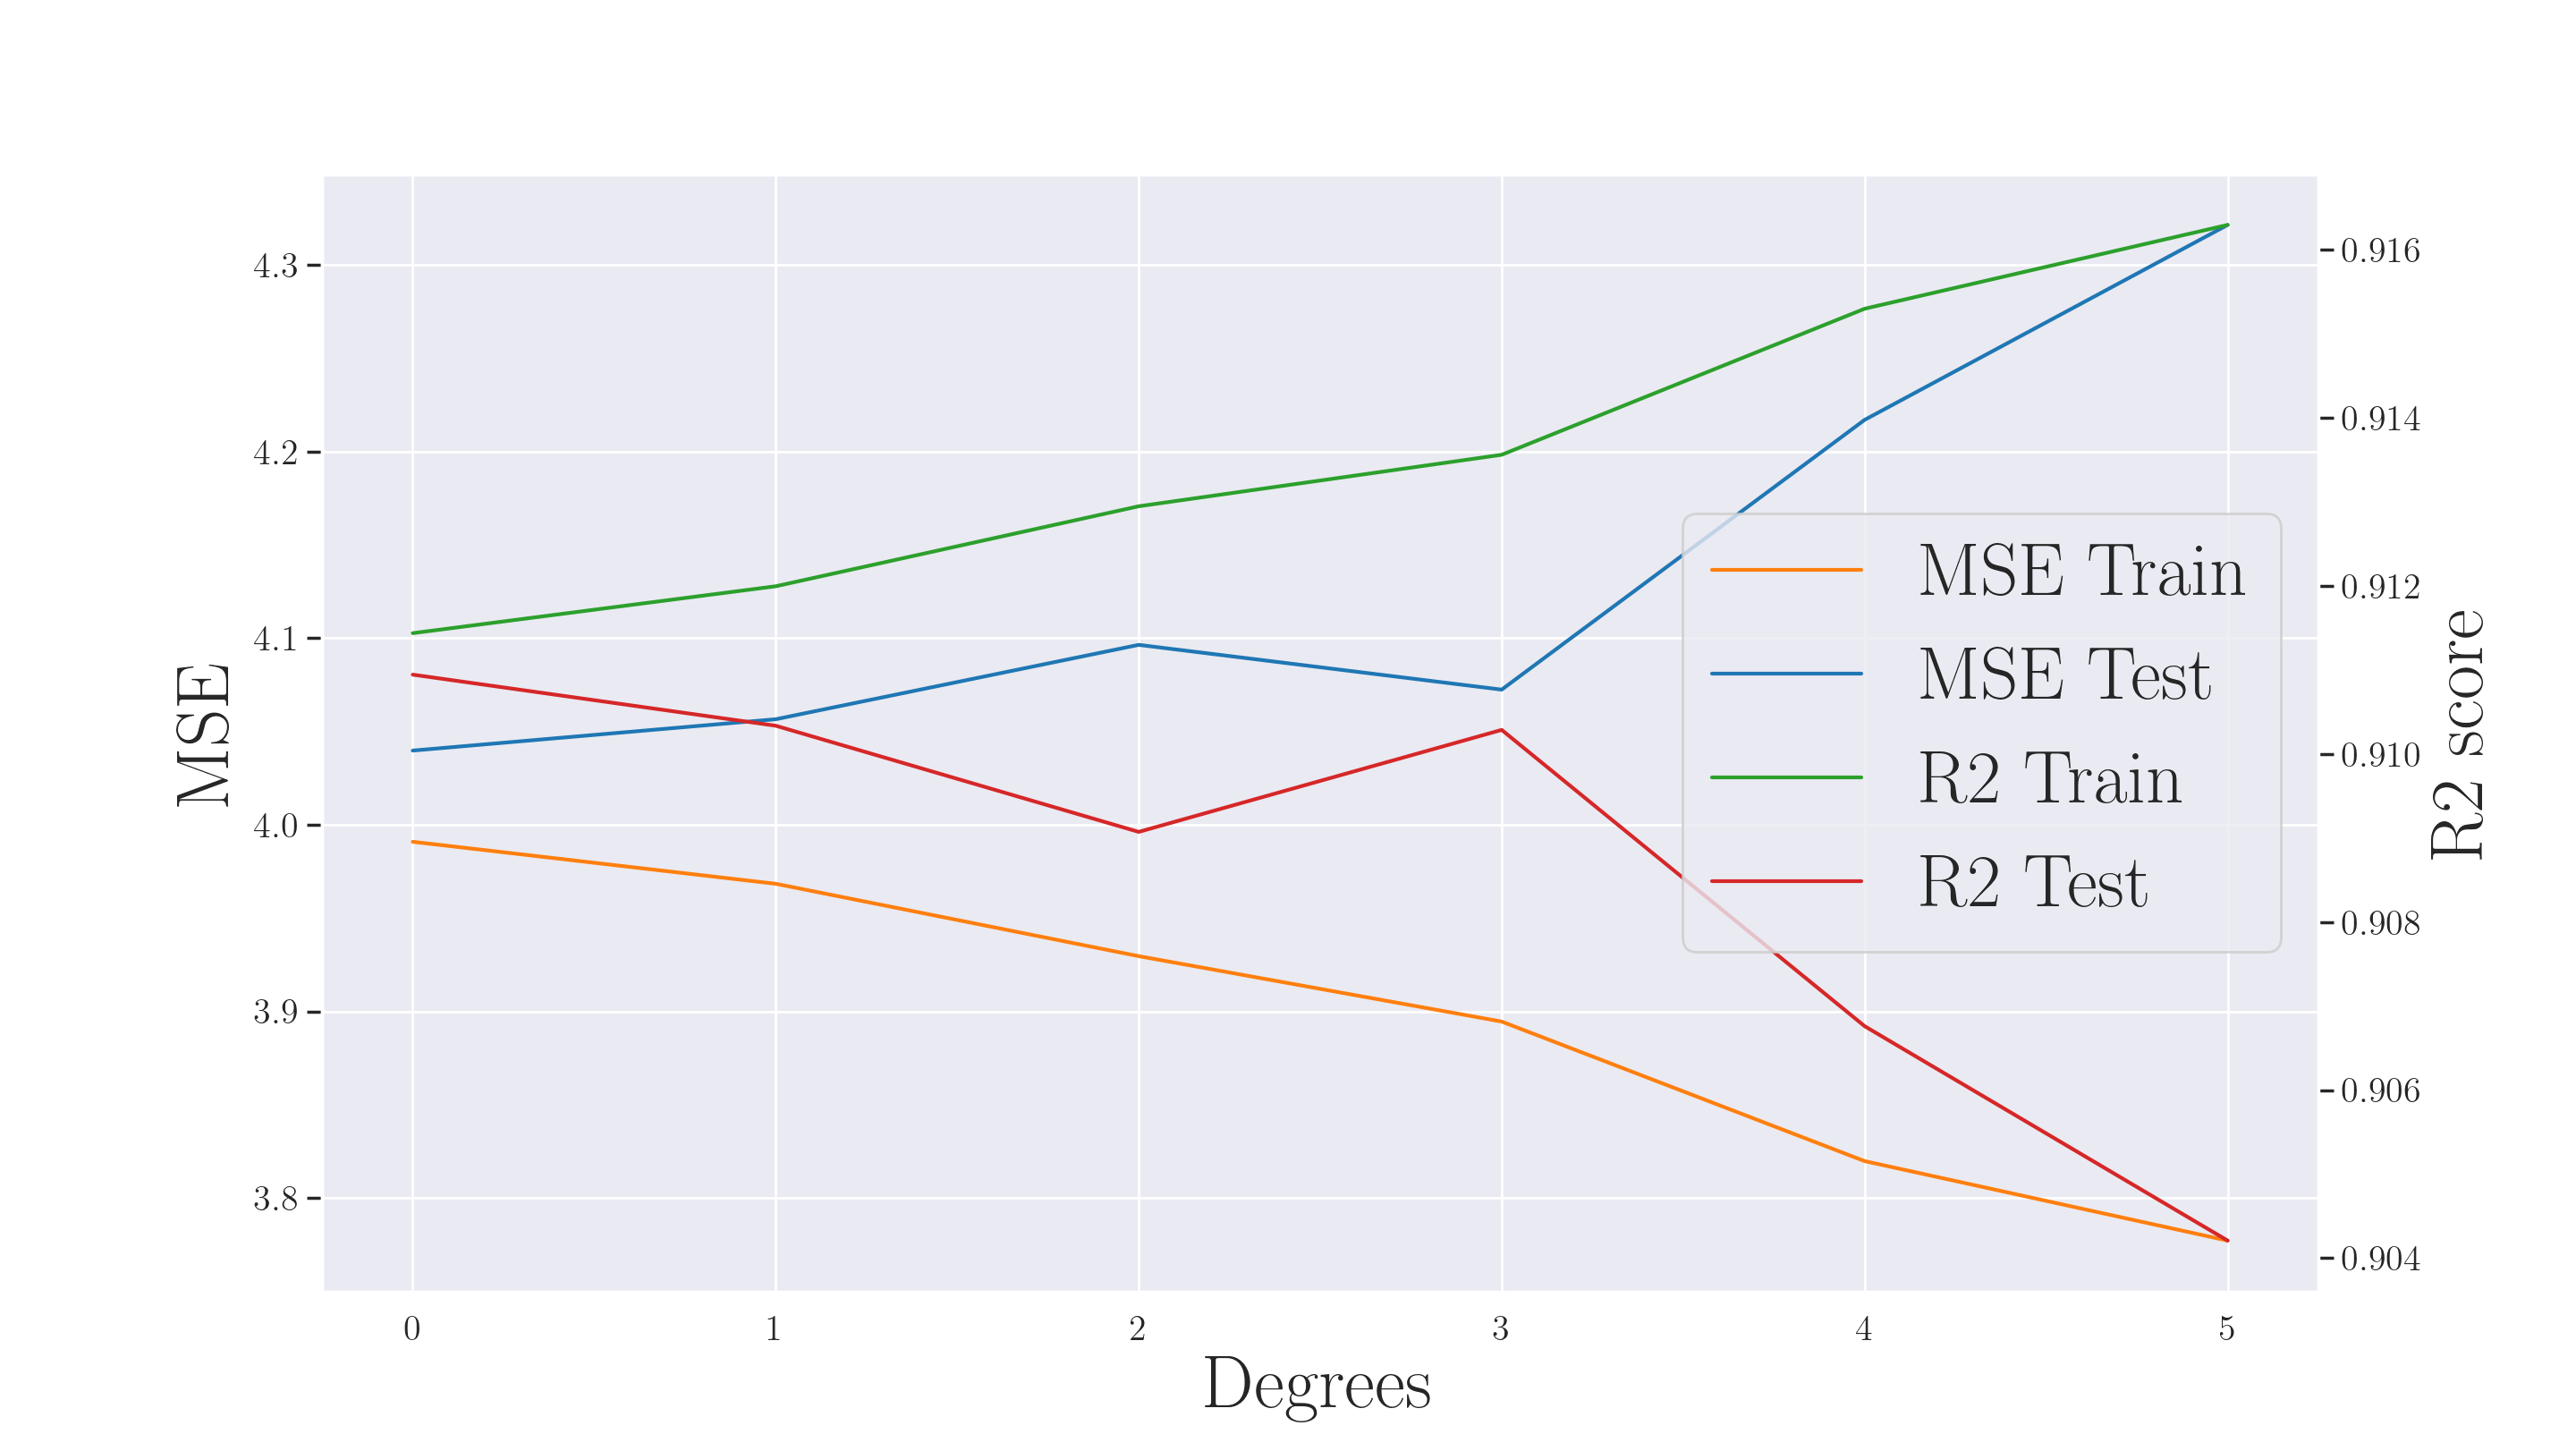
\includegraphics[width=\linewidth]{images/Figure_16.png}
	\caption{A plot of the MSE and R2 score as a function of degrees and a $\lambda$ value of $10^{-5}$ for Ridge regression on the Franke function with noise given by the normal distribution $\mathcal{N}(0,0.1)$.}
	\label{MSE and R2 Ridge noise}
\end{figure}
\noindent We can also see what happens for the ridge regression if $\lambda$ is put to zero. Figure \eqref{MSE and R2 Ridge noise lambda0} shows the MSE and R2 score if $\lambda = 0$, while figure \eqref{Ridge vs OLS} shows the MSE if $\lambda = 0$ and $\lambda = 10^{-5}$. 
\begin{figure}[H]
	\centering
	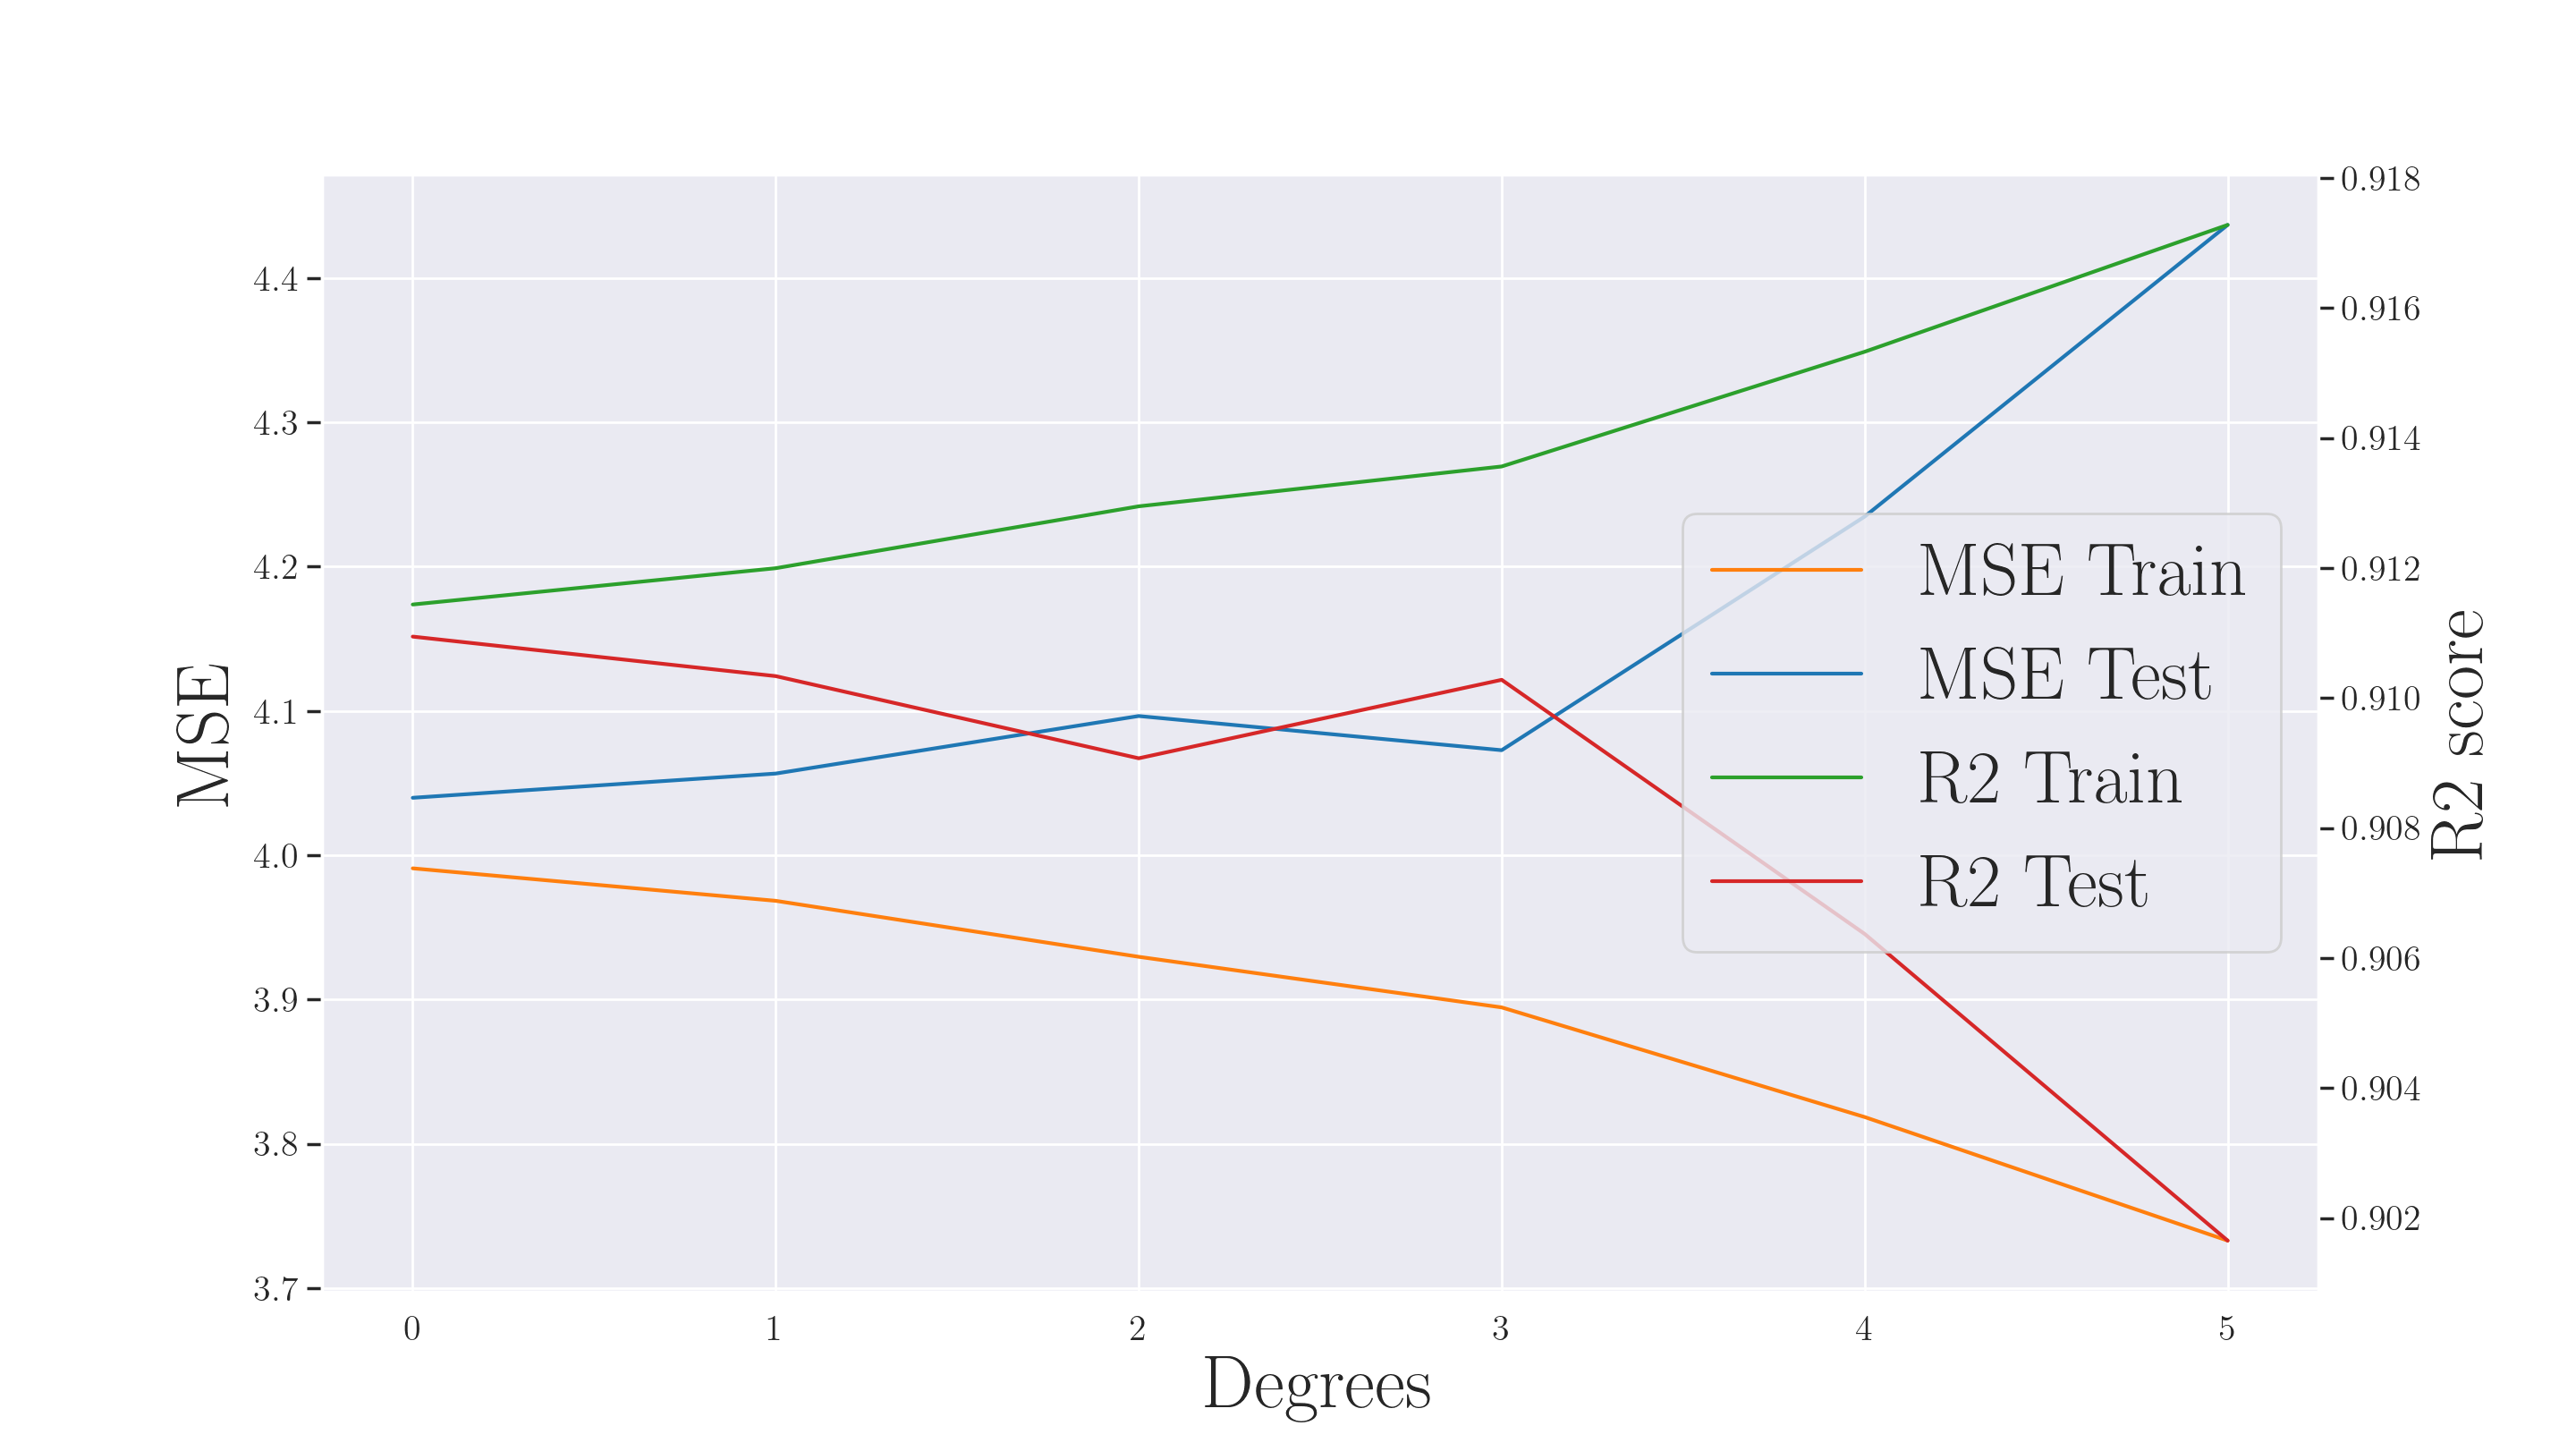
\includegraphics[width=\linewidth]{images/Figure_17.png}
	\caption{A plot of the MSE and R2 score as a function of degrees and a $\lambda$ value of $0$ for Ridge regression on the Franke function with noise given by the normal distribution $\mathcal{N}(0,0.1)$.}
	\label{MSE and R2 Ridge noise lambda0}
\end{figure}
\begin{figure}[H]
	\centering
	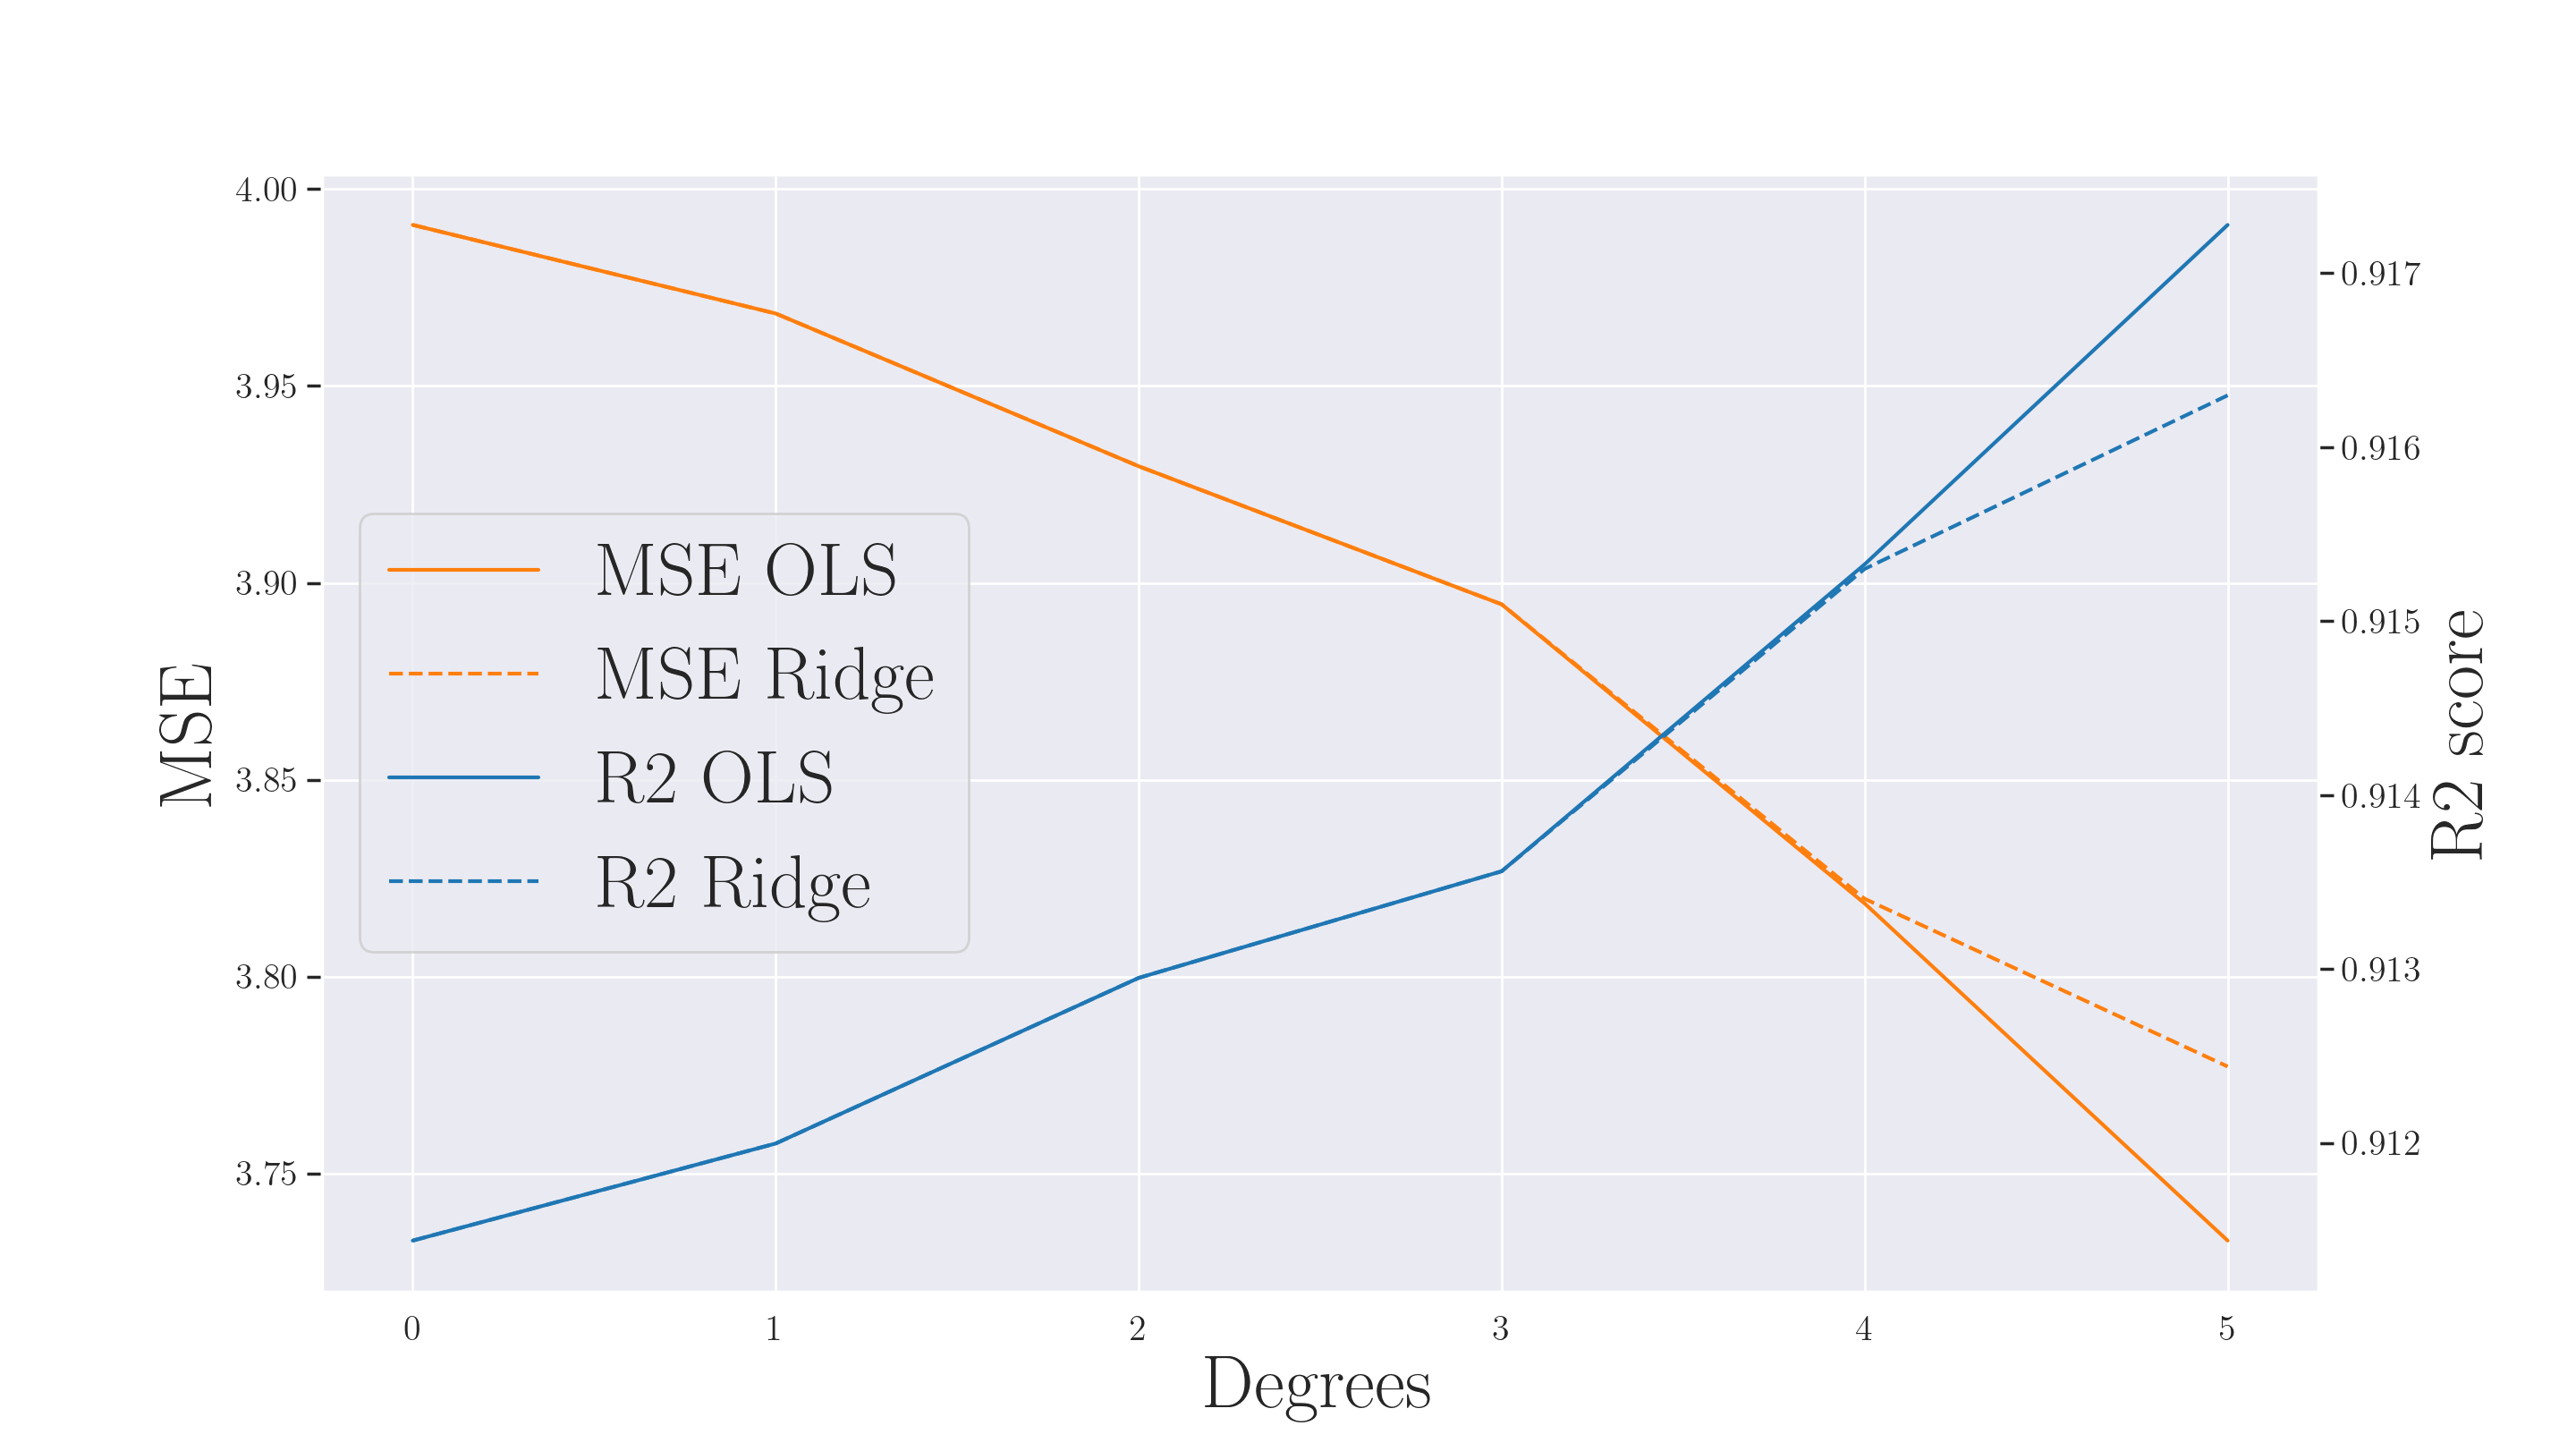
\includegraphics[width=\linewidth]{images/Figure_19.png}
	\caption{A plot of Ridge regression were solid lines shows when $\lambda = 0$, so the same as OLS and the one with doted lines is for $\lambda = 10^{-5}$.}
	\label{Ridge vs OLS}
\end{figure}

\noindent In Figure \eqref{Ridge_crossval_mse_deg} the Mean Squared Error (MSE) is depicted on the $y$-axis, with the logarithm to the base 10 of the hyper parameter $\lambda$ ($\log_{10}(\lambda)$). For the $x$-axis we set the polynomial degrees ranging from 0 - 15. Different lines in varying colors are plotted to showcase the MSE across different $\lambda$ values.
%
\begin{figure}[H]
	\centering
	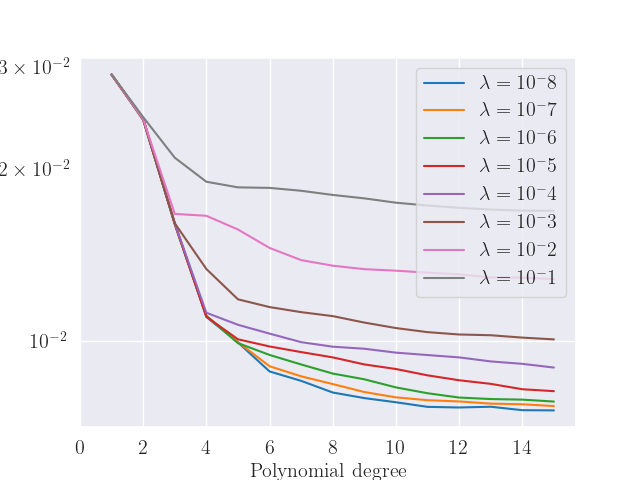
\includegraphics[width=\linewidth]{images/cv_ridge.png}
	\caption{MSE of ridge prediction error for polynomial degree $0-15$, using the Franke function, with cross validation $k=5$.}
 \label{Ridge_crossval_mse_deg}
\end{figure}
%
\noindent Lastly for Ridge regression we plot the $\beta$ values for different complexities in figure \eqref{beta Ridge}. 
\begin{figure}[H]
	\centering
	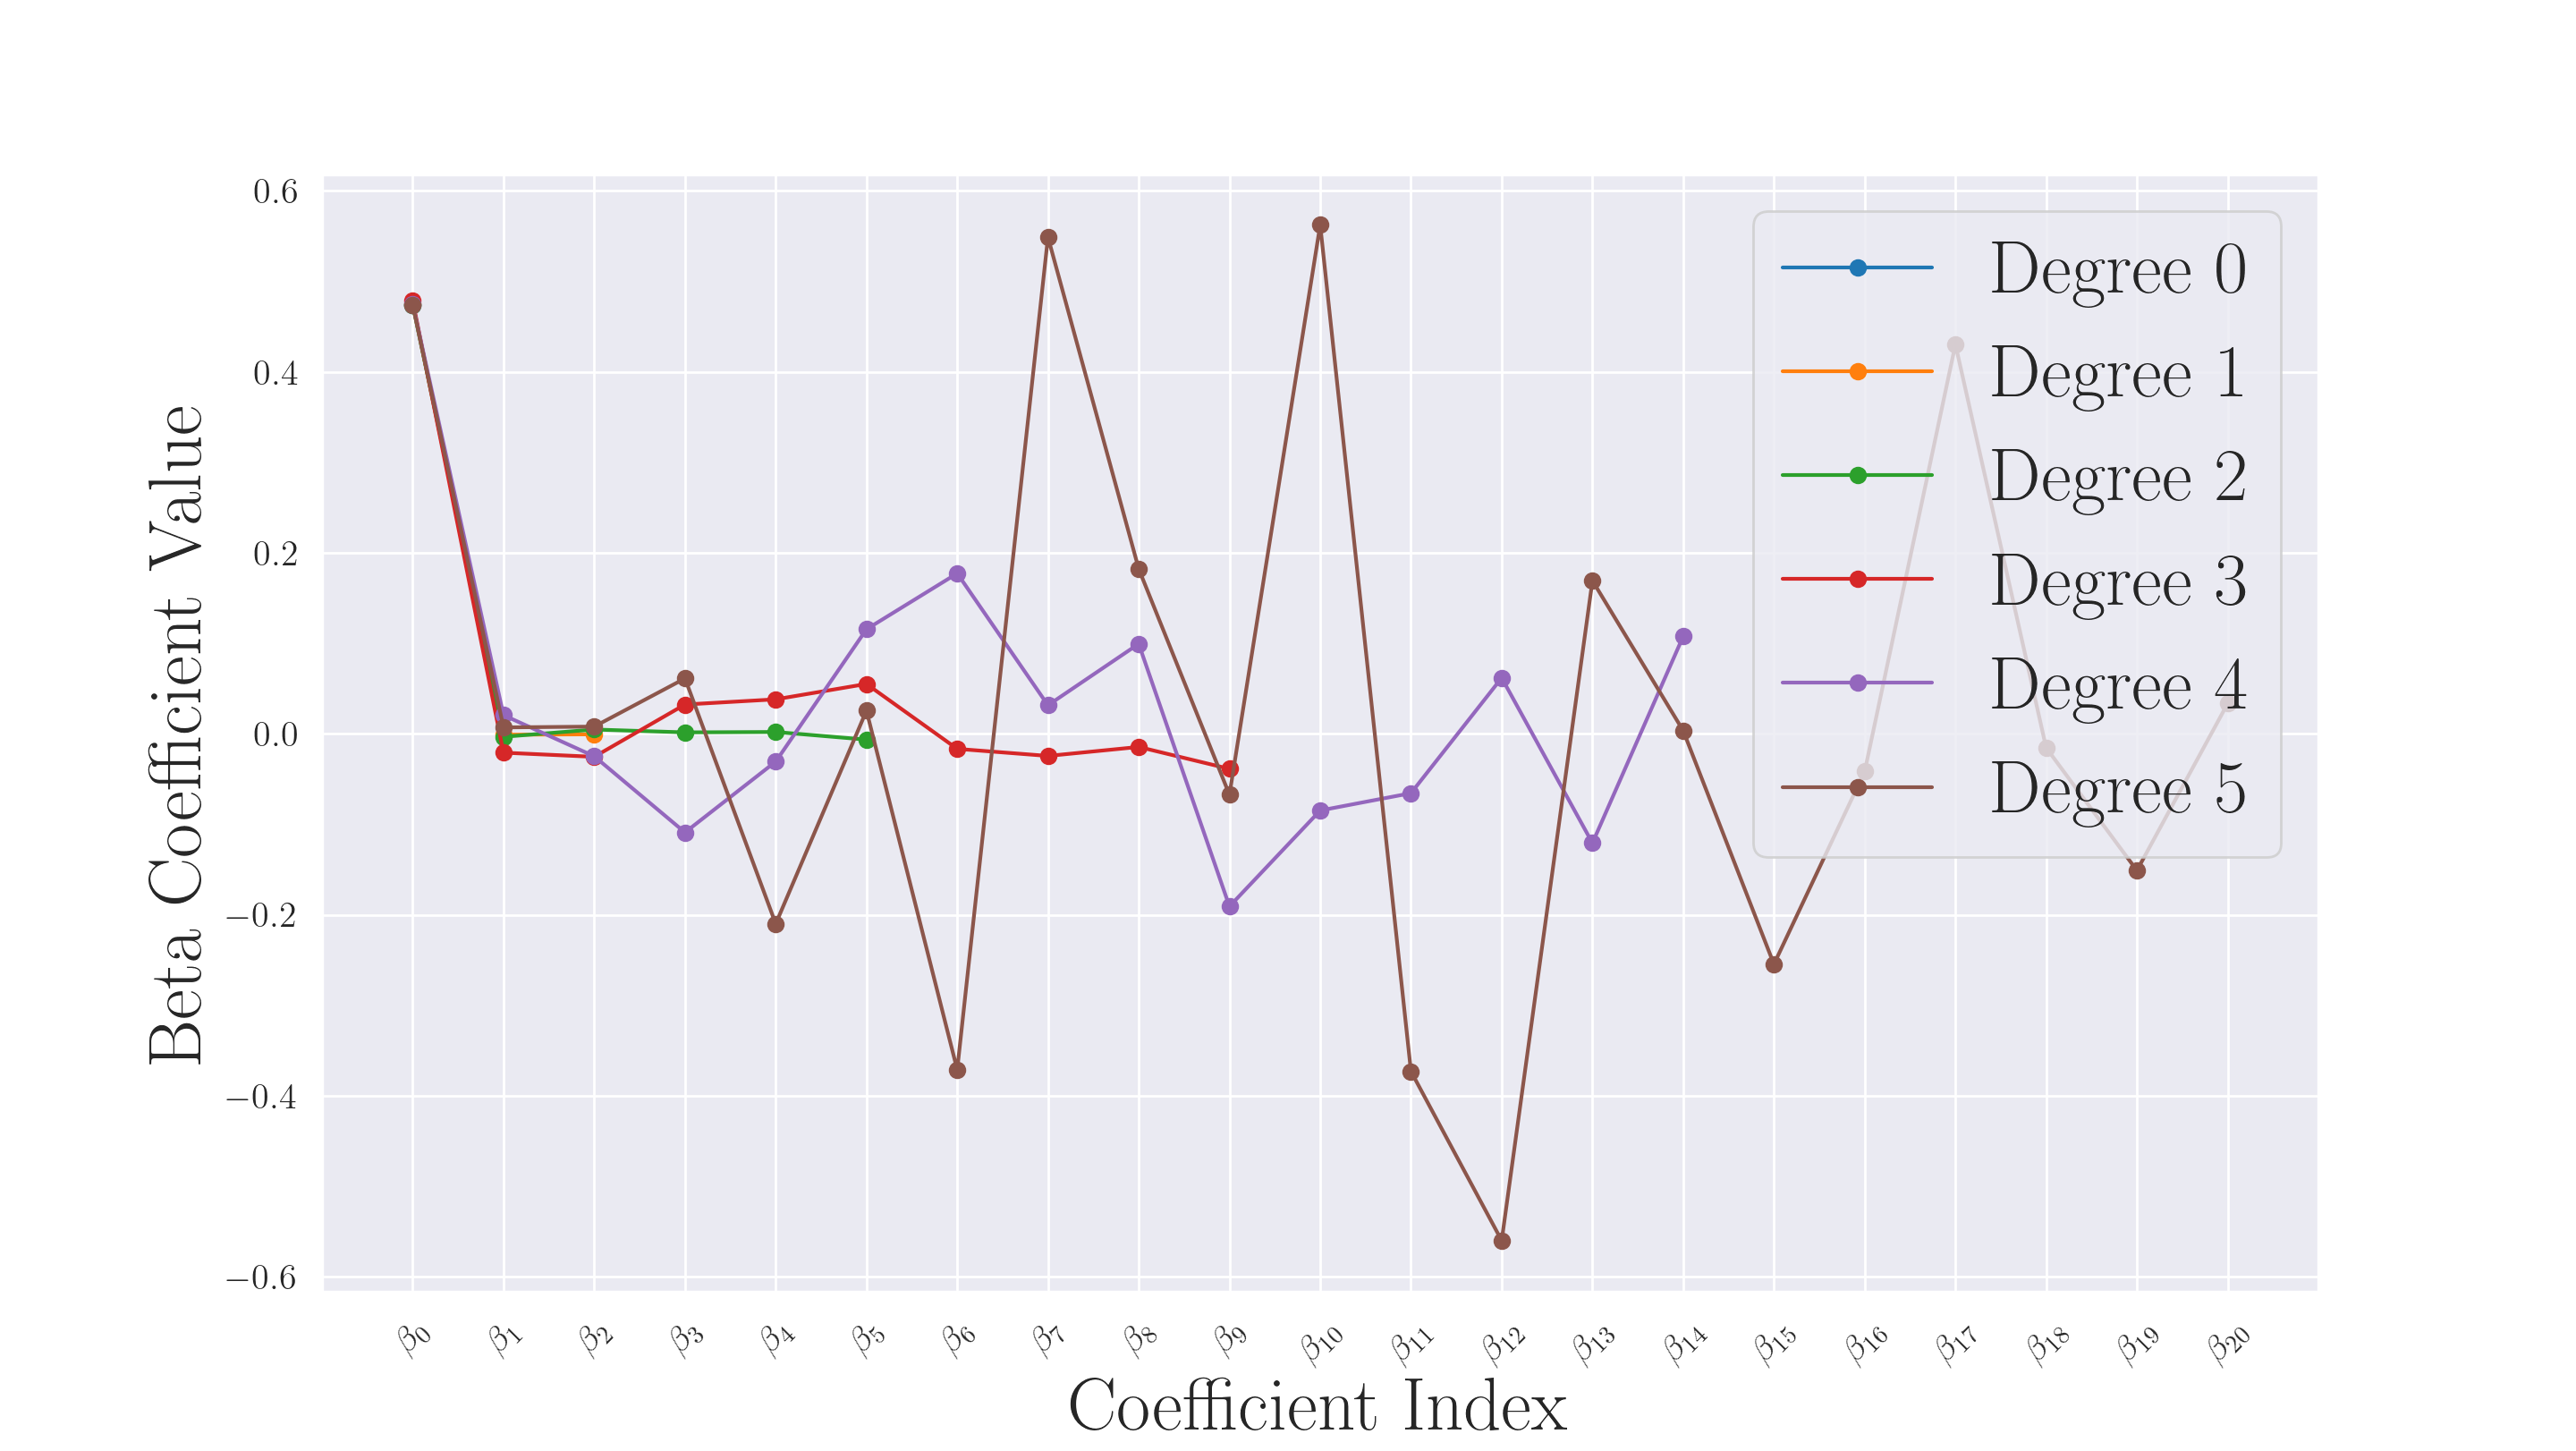
\includegraphics[width=\linewidth]{images/Figure_34.png}
	\caption{A plot showing the $\beta$ values for OLS for different orders of polynomials.}
	\label{beta Ridge}
\end{figure}

\subsubsection{LASSO}
\noindent For LASSO regression we started by making heat maps for both the training data (figure \eqref{heat map training LASSO}) and test data (figure \eqref{heat map test LASSO}) with the same $\lambda$ values ($10^{-8}$ to $10^{2}$) and polynomial degrees (1-5) like for Ridge regression .

\begin{figure}[H]
	\centering
	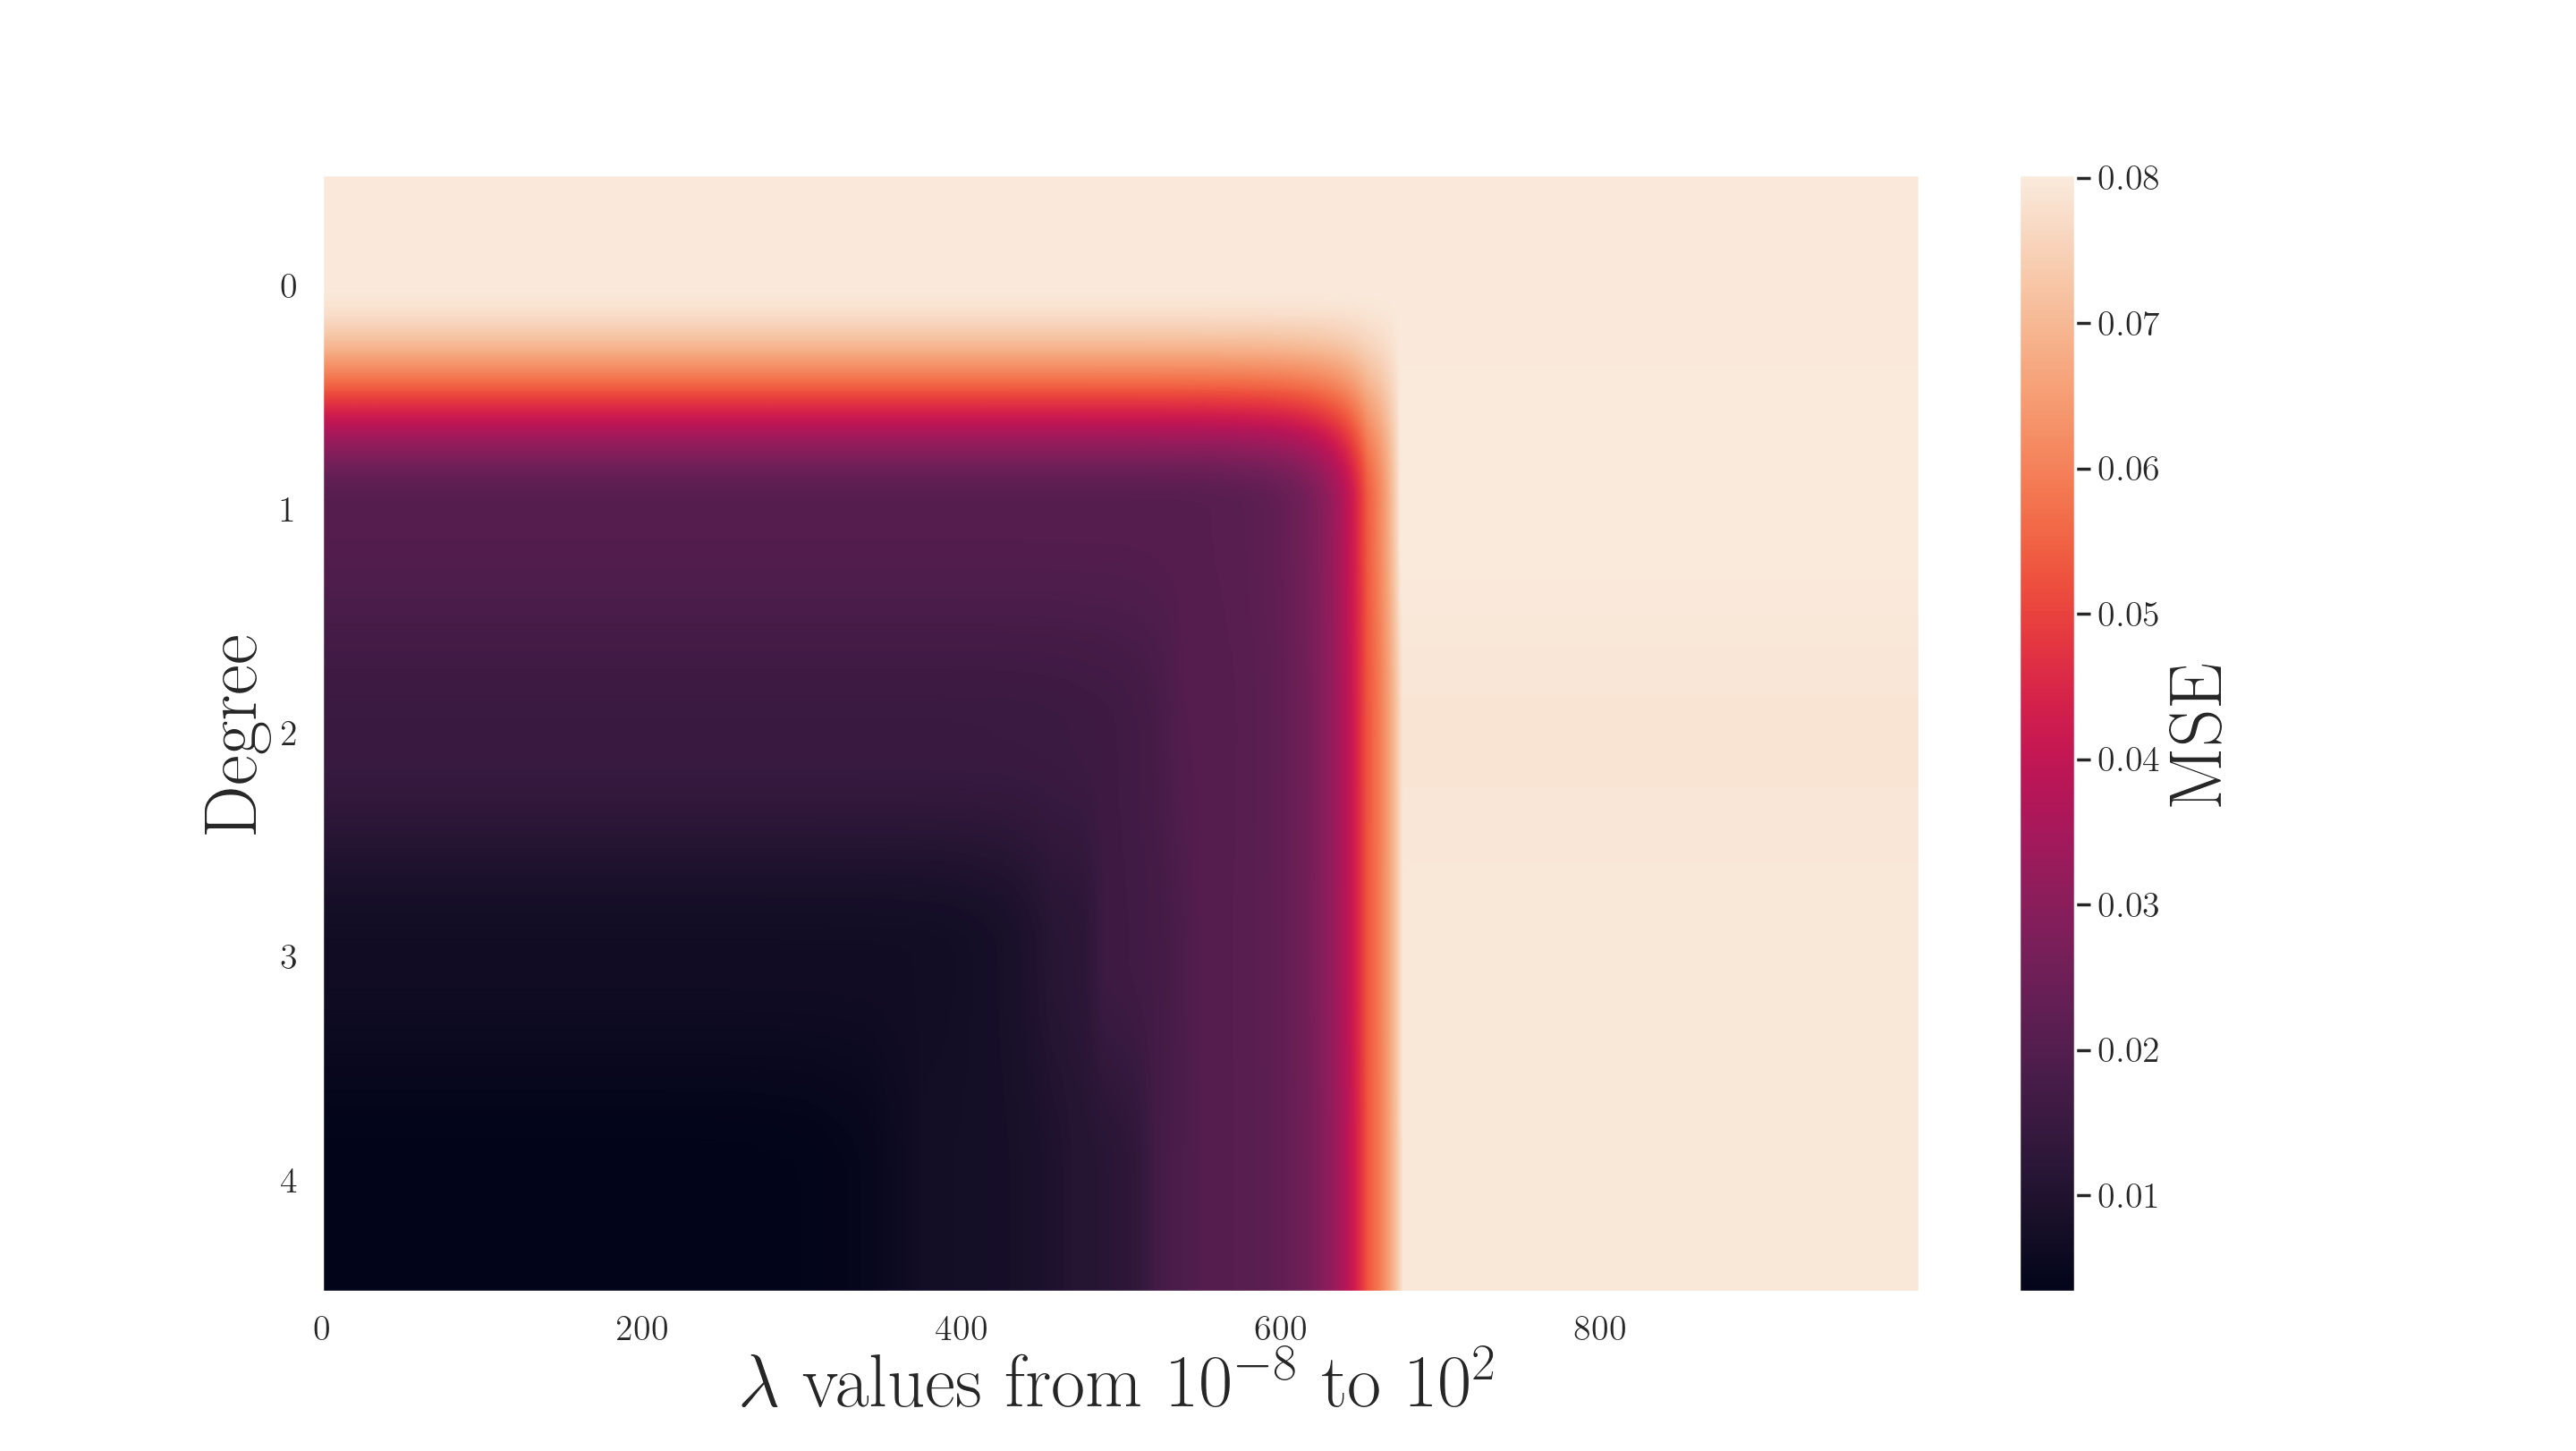
\includegraphics[width=\linewidth]{images/Figure_9.png}
	\caption{A heat map of the MSE for the training data, for different $\lambda$ values and complexities. The $\lambda$ values goes from $10^{-8}$ to $10^{2}$. }
	\label{heat map training LASSO}
\end{figure}
%
\begin{figure}[H]
	\centering
	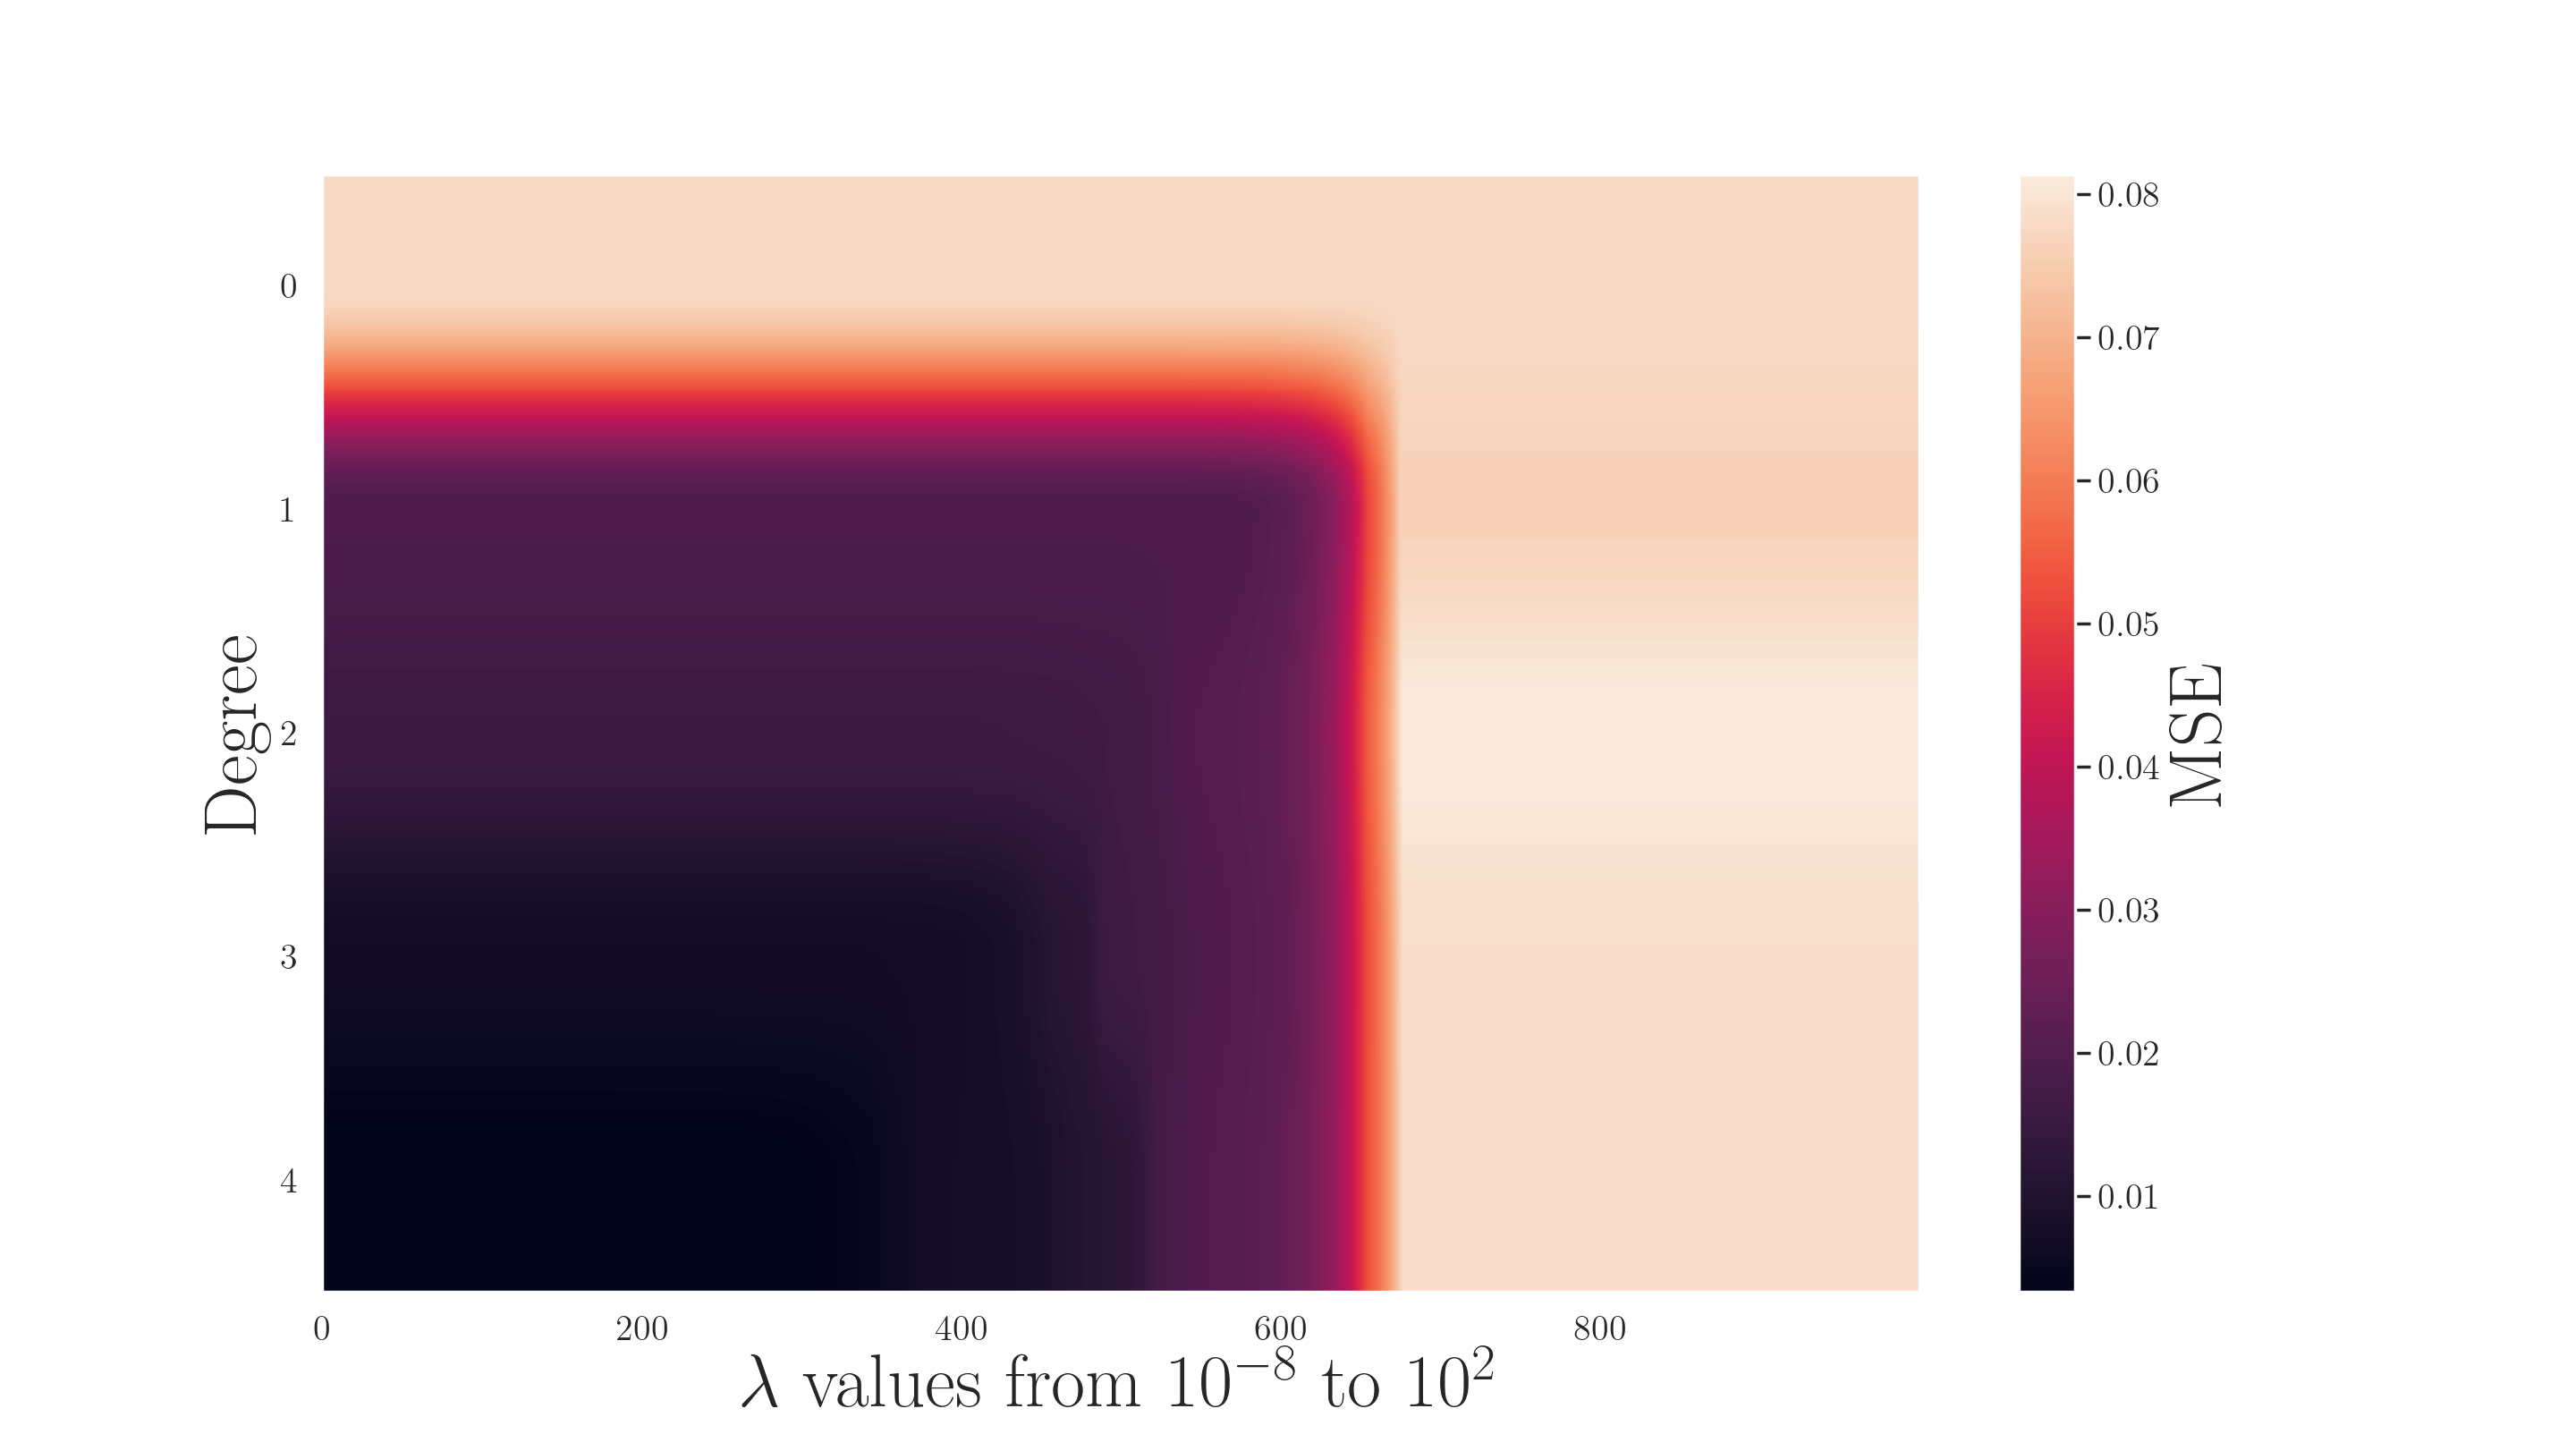
\includegraphics[width=\linewidth]{images/Figure_10.png}
	\caption{A heat map of the MSE for the testing data, for different $\lambda$ values and complexities. The $\lambda$ values goes from $10^{-8}$ to $10^{2}$.}
	\label{heat map test LASSO}
\end{figure}
%
\noindent We then plotted the MSE and R2 score as a function of complexity both without noise (figure \eqref{MSE_and_R2_Lasso_no_noise}) and with noise given by the normal distribution $\mathcal{N}(0,0.1)$ (figure \eqref{MSE_and_R2_Lasso_noise}) for $\lambda = 10^{-5}$.
%
\begin{figure}[H]
    \centering
    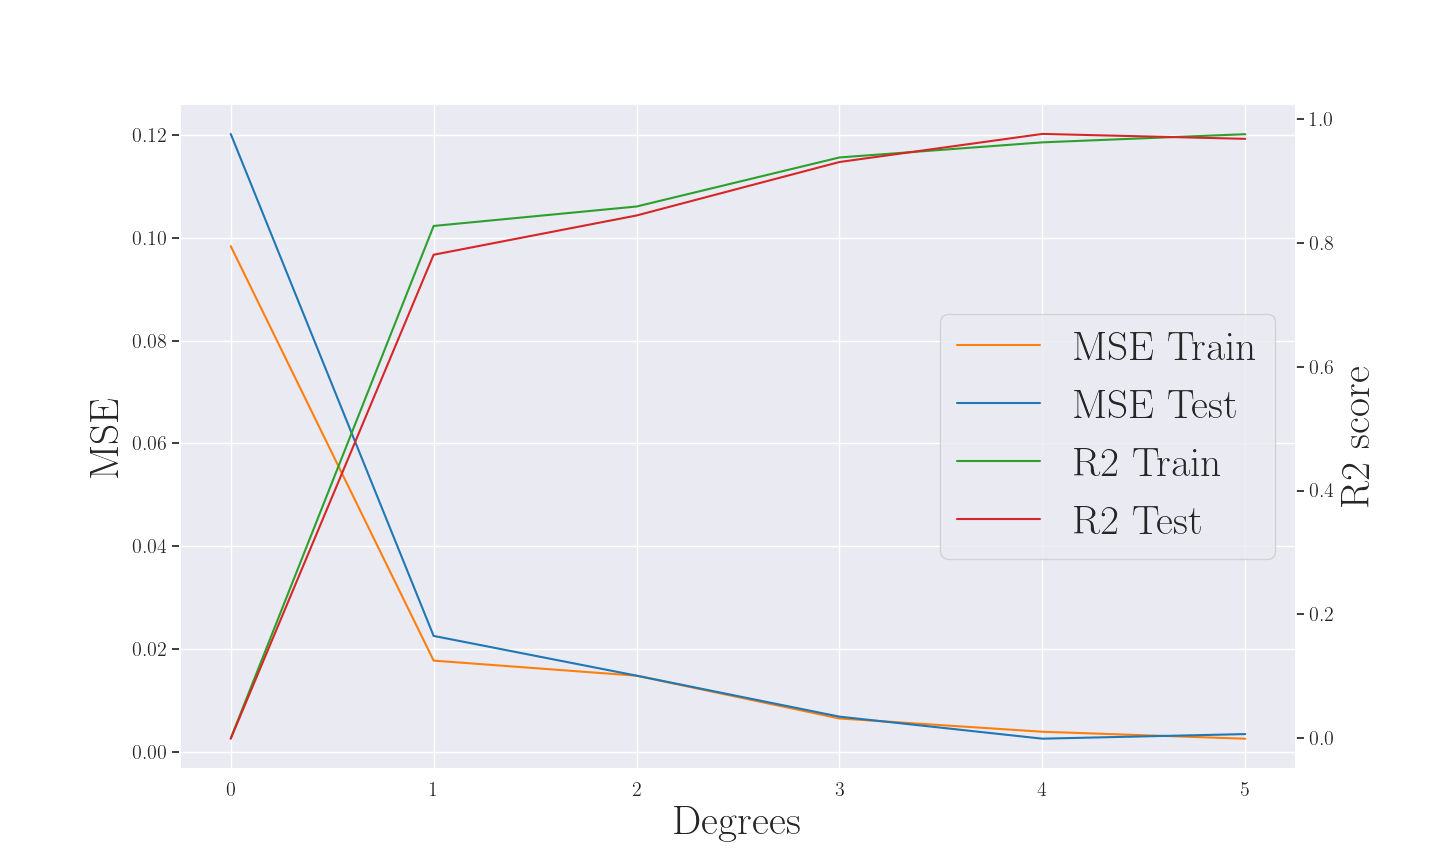
\includegraphics[width=\linewidth]
    {images/MSE_and_R2_Lasso.png}
    \caption{A plot of the MSE and R2 score as a function of degrees and a $\lambda$ value of $10^{-5}$ for LASSO regression on the Franke function with no noise present.} \label{MSE_and_R2_Lasso_no_noise}
\end{figure}
%
\begin{figure}[H]
    \centering
    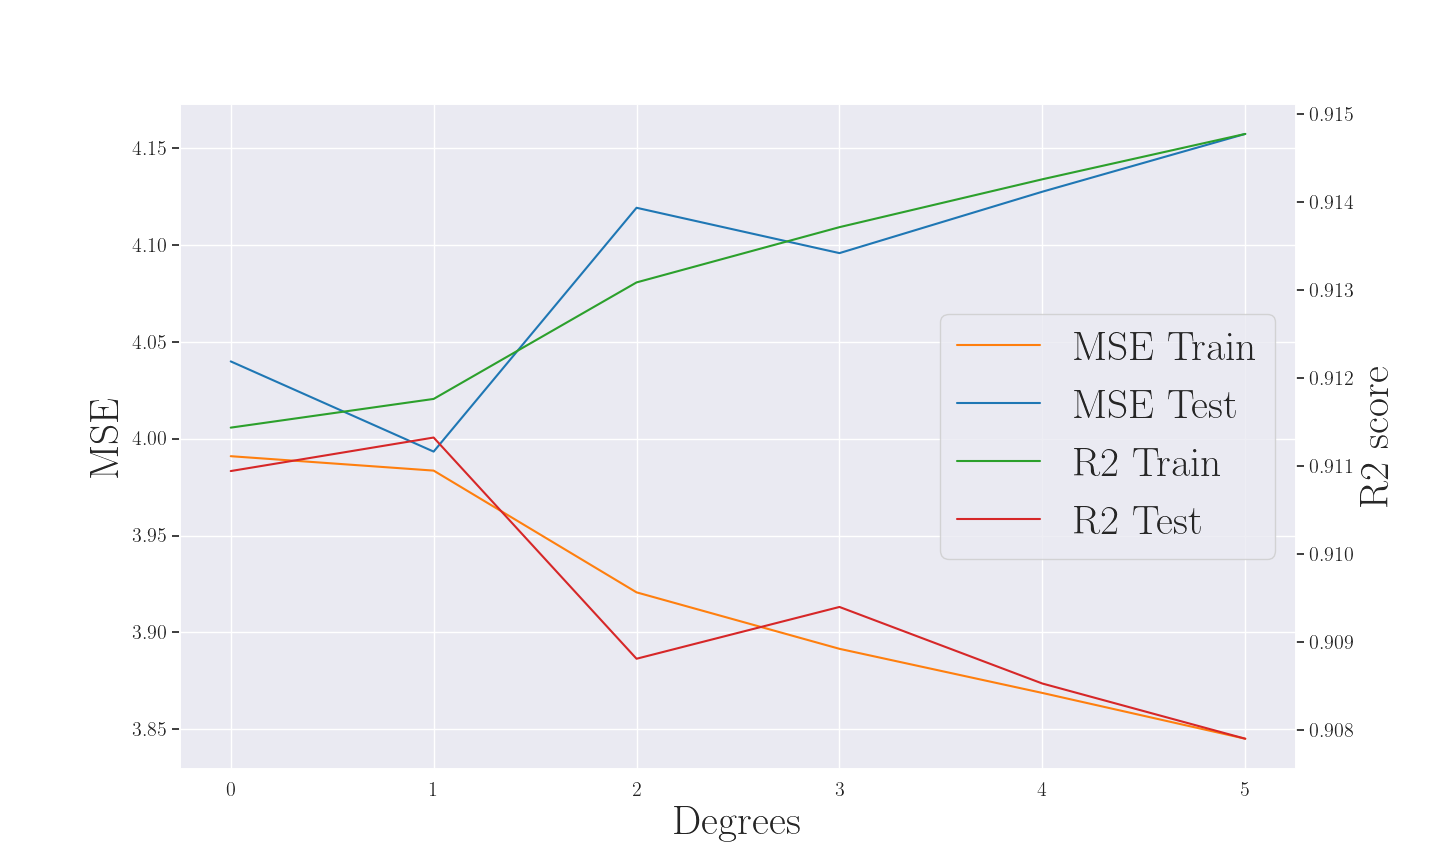
\includegraphics[width=\linewidth]{images/MSE_and_R2_Lasso_noise.png}
    \caption{A plot of the MSE and R2 score as a function of degrees and a $\lambda$ value of $10^{-5}$ for LASSO regression on the Franke function with noise given by the normal distribution $\mathcal{N}(0,0.1)$.} \label{MSE_and_R2_Lasso_noise}
\end{figure}
%
\noindent We then plotted the MSE for OLS, Ridge ($\lambda = 10^{-5}$) and LASSO ($\lambda = 10^{-5}$) given in figure \eqref{OLS_Ridge_and_Lasso} . 
%
\begin{figure}[H]
	\centering
	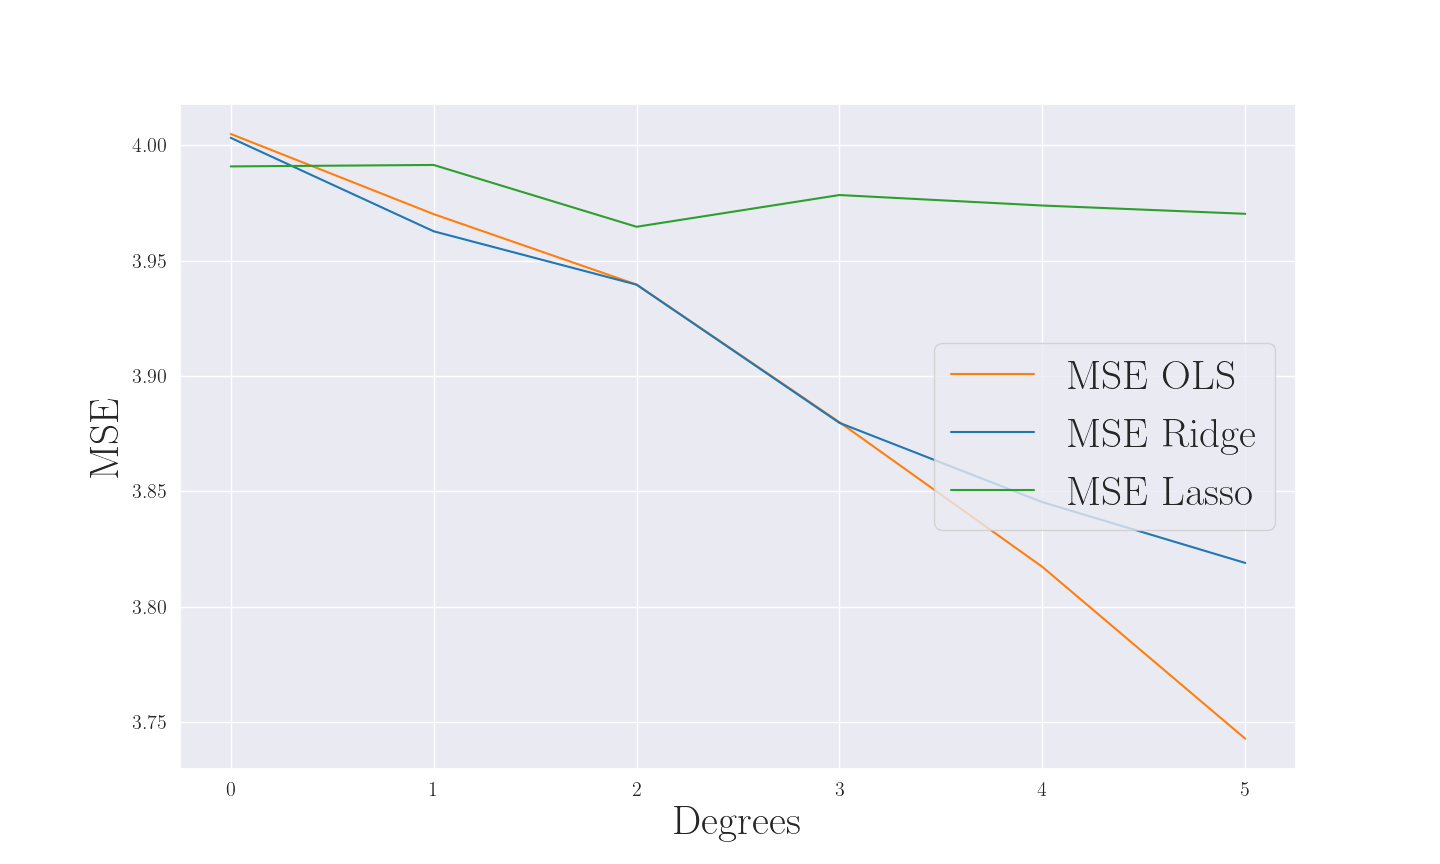
\includegraphics[width=\linewidth]{images/MSE_for_OLS_Ridge_Lasso.png}
	\caption{A plot of OLS, Ridge regression with $\lambda = 10^{-5}$ and LASSO regression with $\lambda = 10^{-5}$ on the Franke function with noise given by the normal distribution $\mathcal{N}(0,0.1)$. }
	\label{OLS_Ridge_and_Lasso}
\end{figure}
%
\noindent In Figure \eqref{Lasso_crossval_mse_deg}, the Mean Squared Error (MSE) is plotted on the $y$-axis in a logarithmic scale. The $x$-axis represents the polynomial degrees, which range from 0 to 14. Multiple colored lines are shown, each representing a specific value of the regularization parameter $\lambda$. These lines provide a visual representation of the MSE across different $\lambda$ values for varying polynomial degrees, assisting in the determination of an optimal polynomial degree and regularization parameter for LASSO regression.
%
\begin{figure}[H]
	\centering
	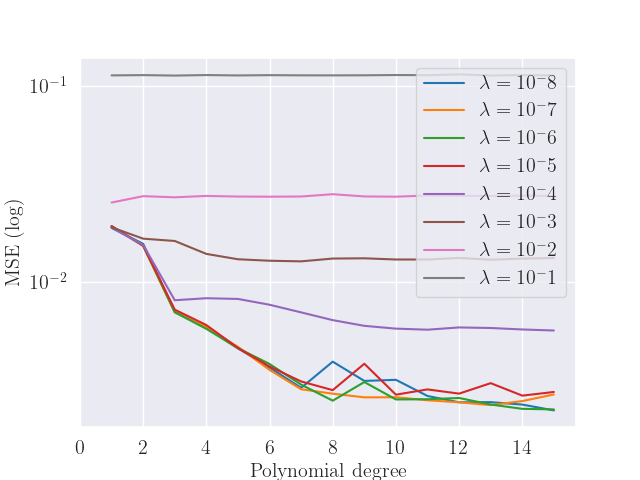
\includegraphics[width=\linewidth]{images/cv_lasso.png}
	\caption{MSE of LASSO prediction error for polynomial degree $0-15$, using the Franke function, with cross validation $k=5$.}
 \label{Lasso_crossval_mse_deg}
\end{figure}

\subsection{Real terrain data}
\subsubsection{OLS}
\noindent Now we look at the analysis of the real terrain data. First we performed a OLS regression on the data set, where we varied the complexity between 0 and 10 degrees. The MSE and R2 score is shown in figure \eqref{OLS terrain data}. 
\begin{figure}[H]
	\centering
	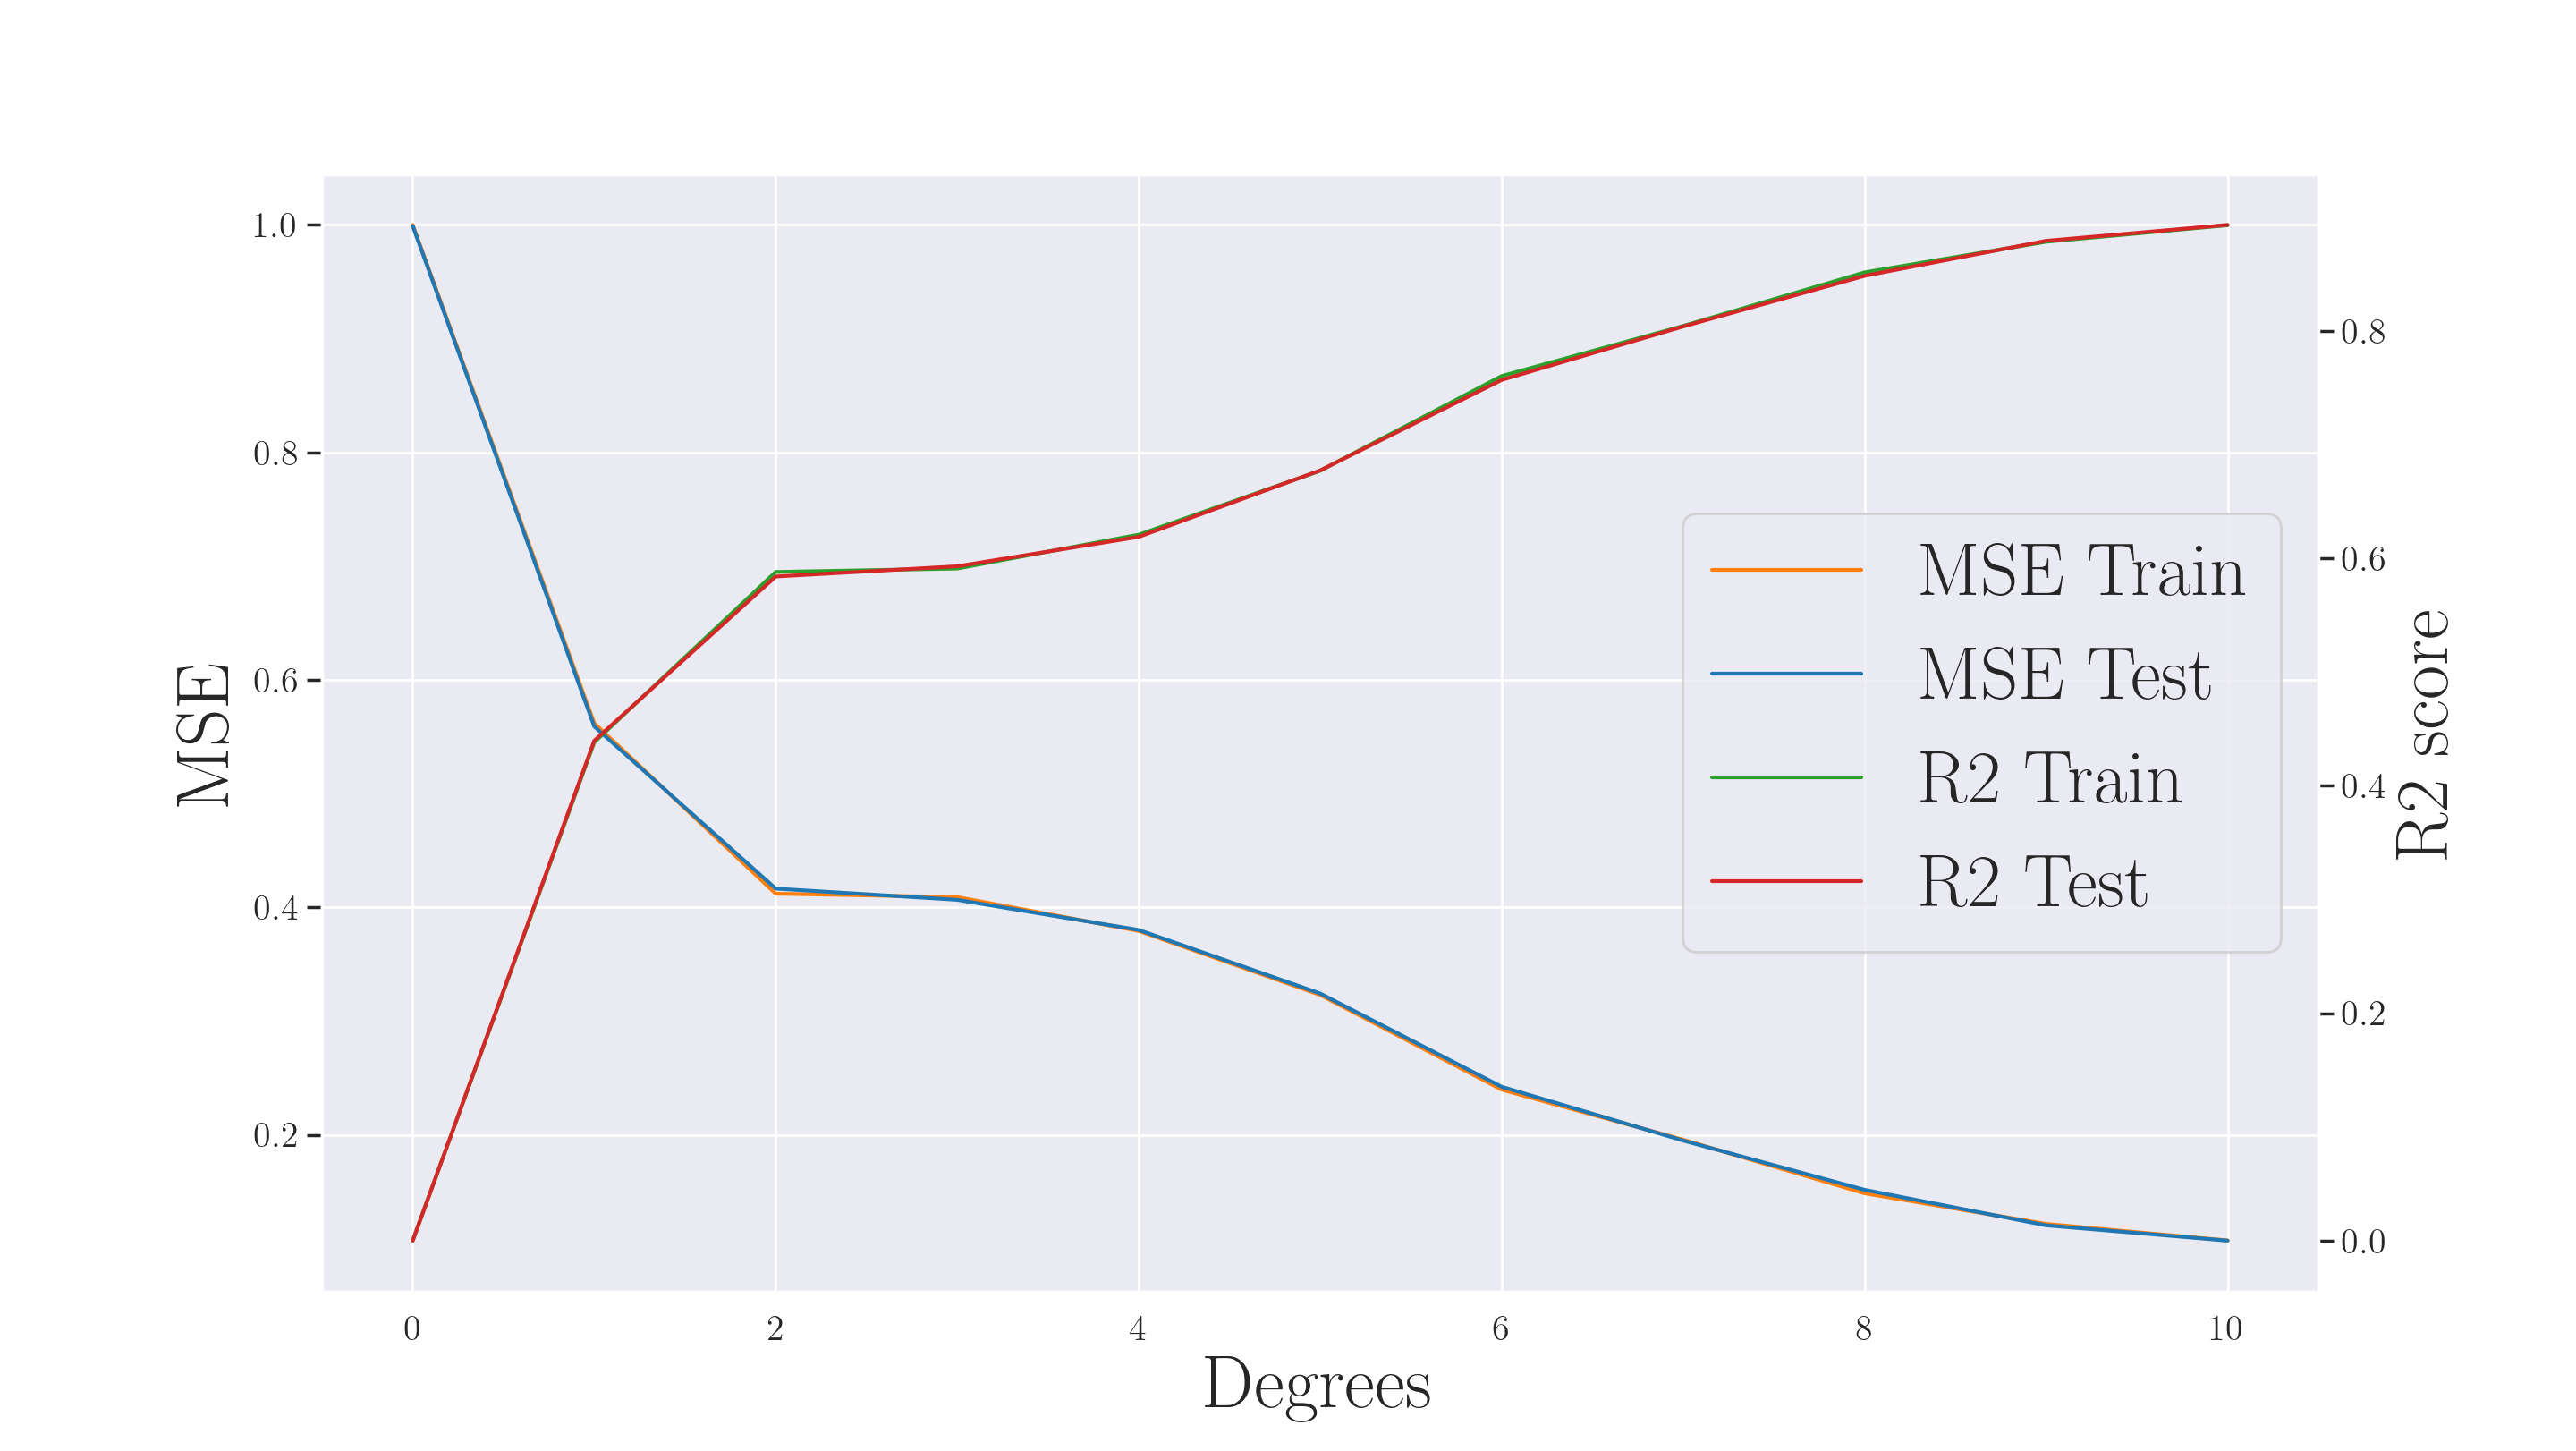
\includegraphics[width=\linewidth]{images/Figure_21.png}
	\caption{A plot showing the MSE and R2 score for the OLS regression on the terrain data.}
	\label{OLS terrain data}
\end{figure}
% Do not think this figura is necerrary since we are comparing Bootstrap and CV in the next figure
% \begin{figure}[H]
%     \centering
%     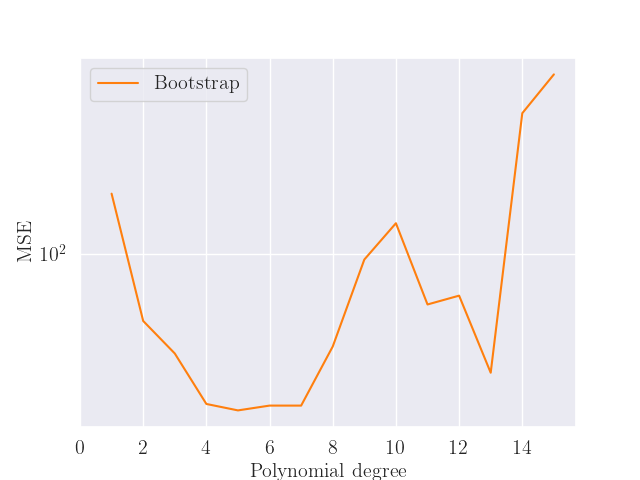
\includegraphics[width=\linewidth]{images/bootstrap_terrain.png}
%     \caption{MSE as a function of complexity for OLS with terrain data, using bootstrap with 100 samples.}
%     \label{fig:bootstrap_terrain}
% \end{figure}
\noindent We compared re-sampling techniques for the terrain data, using OLS as regression method. MSE for both are shown in figure \ref{fig:bootstrap_cv_terrain}. 
\begin{figure}[H]
    \centering
    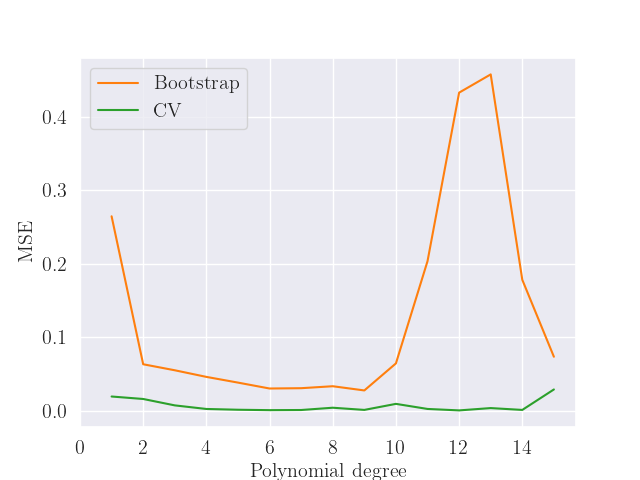
\includegraphics[width=\linewidth]{images/bootstrap_cv_terrain.png}
    \caption{MSE as a function of complexity for OLS with terrain data, using both bootstrap with 100 samples, and cross validation with $k=5$.}
    \label{fig:bootstrap_cv_terrain}
\end{figure}

\subsubsection{Ridge}
\noindent Next we implemented Ridge regression on the terrain data. We made a heat map of the MSE values as a function of $\lambda$ values and complexity. The complexity varied from 1 to 10 and the $\lambda$ values varied from $10^{-8}$ to $10^{2}$. The result is shown in figure \eqref{heat map Ridge Terrain data} and \eqref{heat map Ridge Terrain data test}.
\begin{figure}[H]
	\centering
	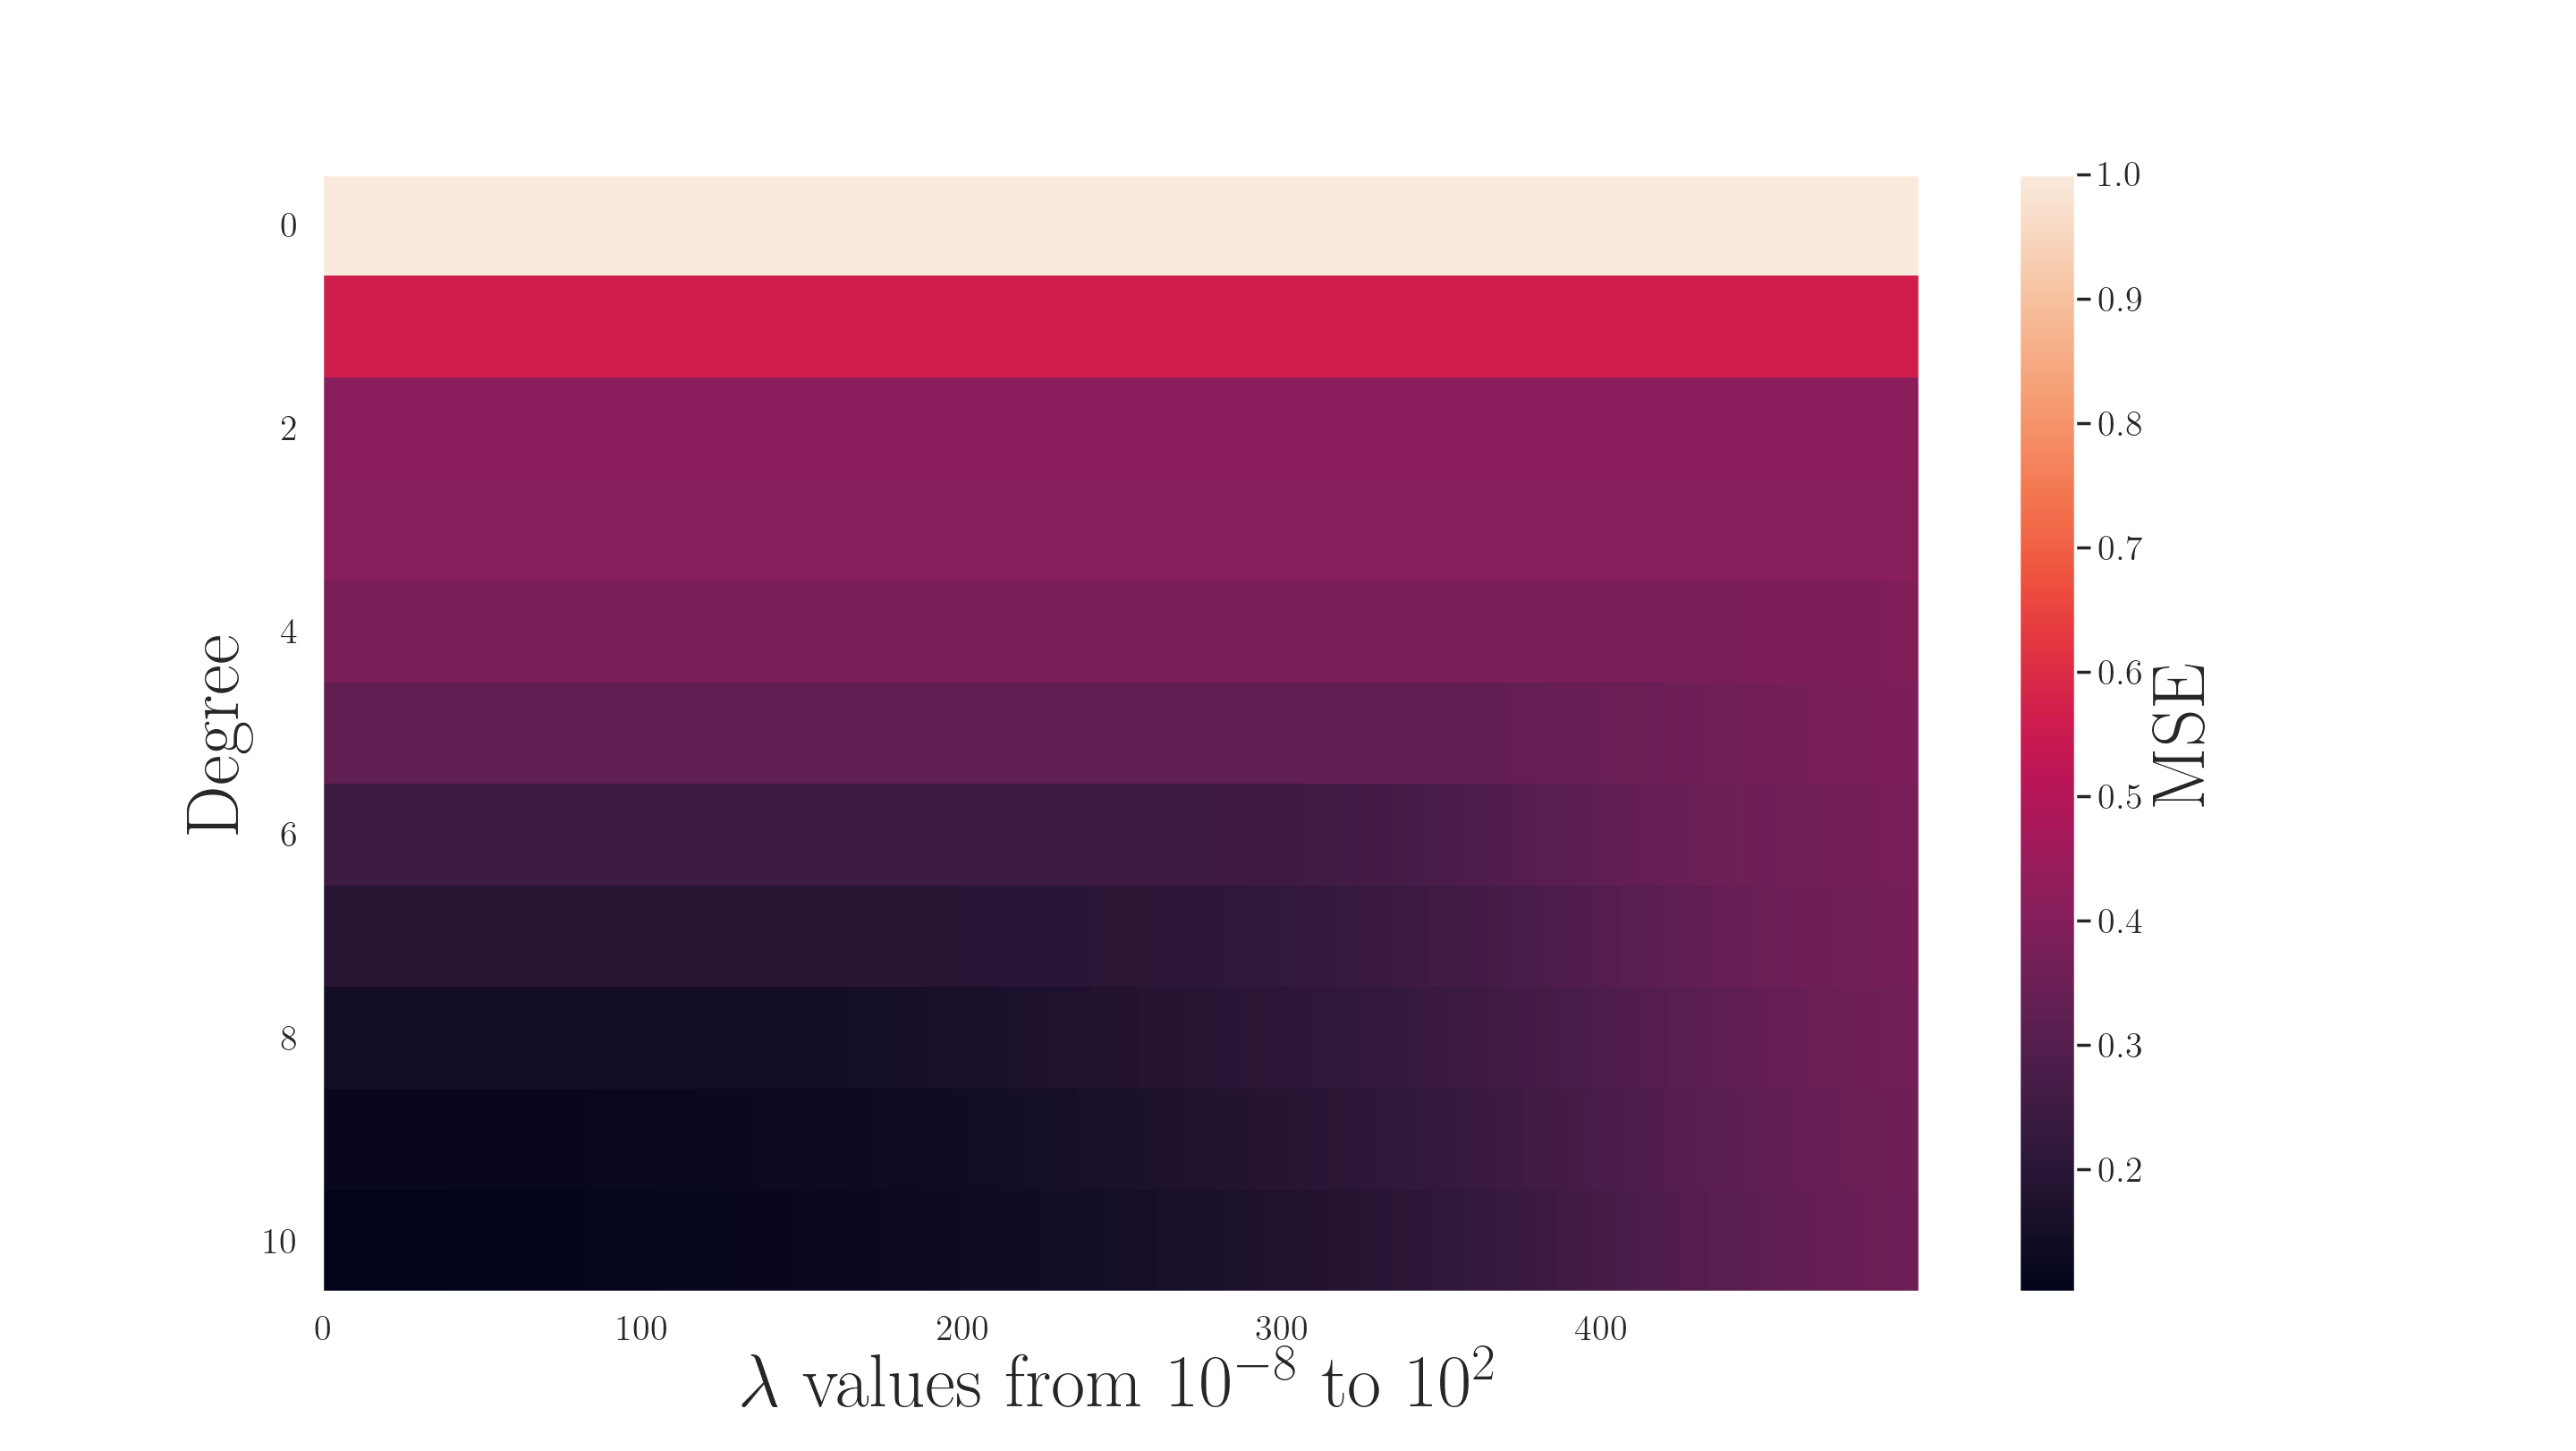
\includegraphics[width=\linewidth]{images/Figure_22.png}
	\caption{Heat map of the MSE for the training data, as a function of complexity and $lambda$ values.}
	\label{heat map Ridge Terrain data}
\end{figure}
%
\begin{figure}[H]
	\centering
	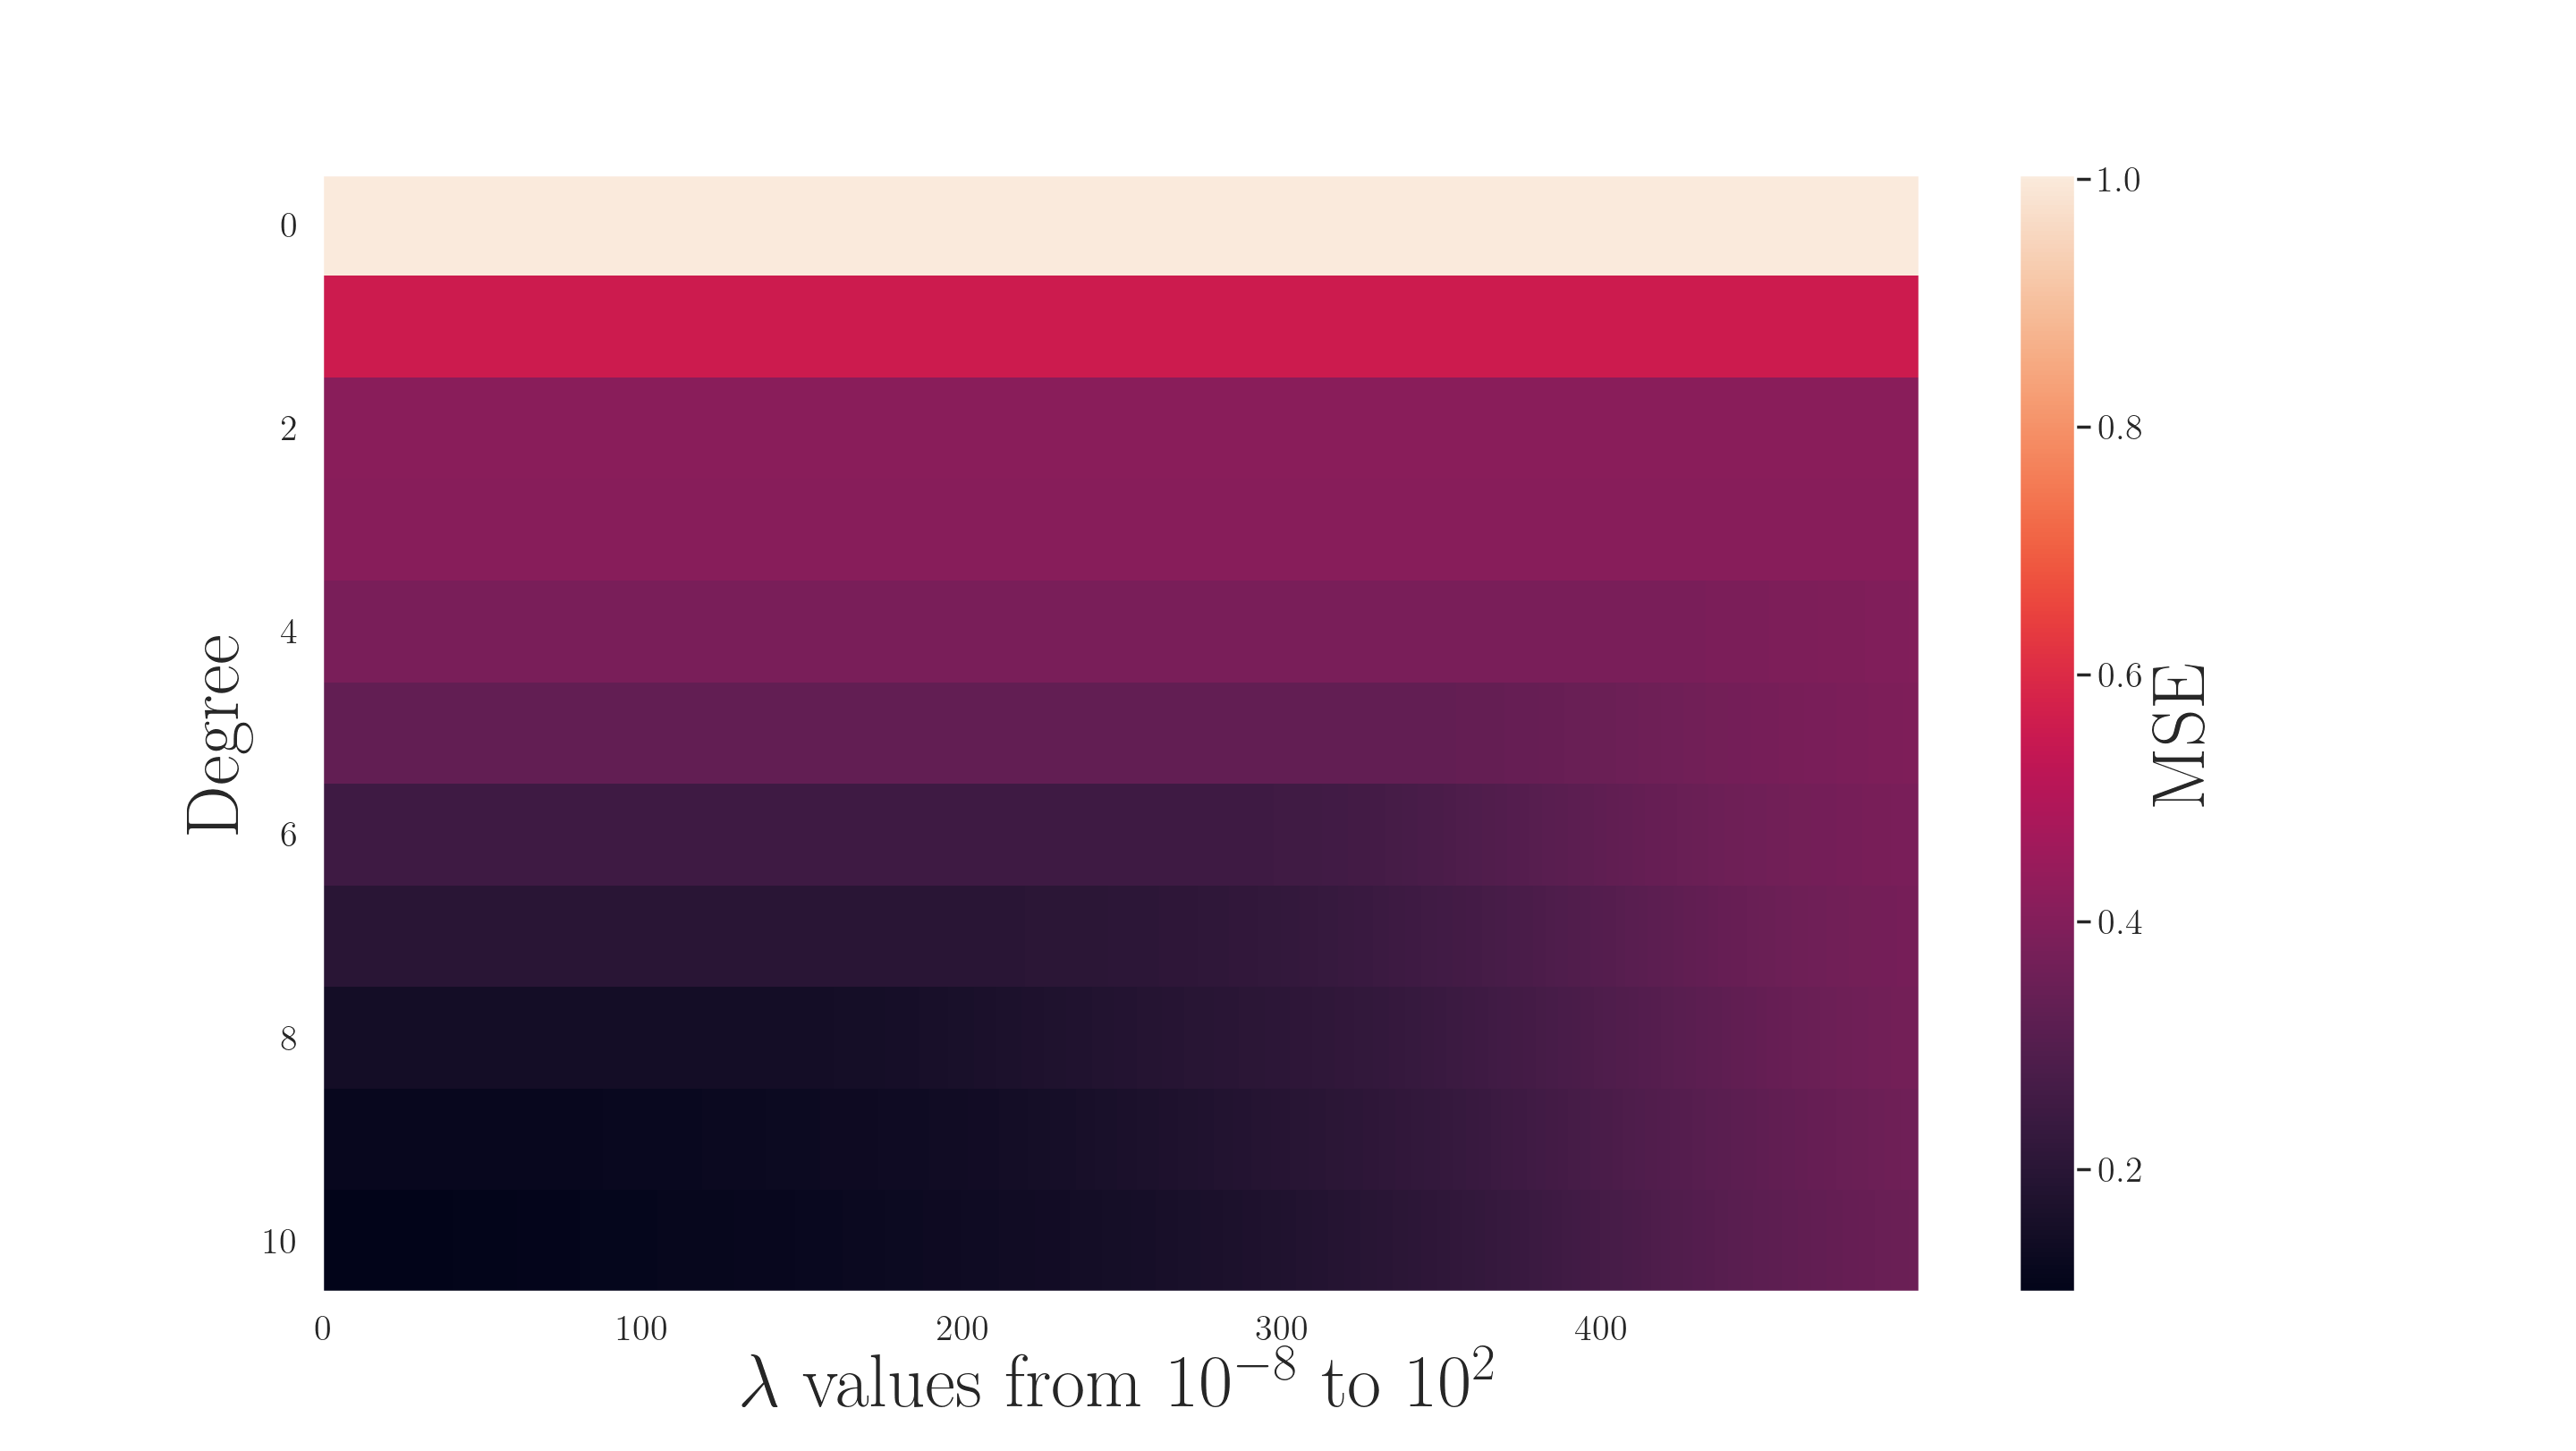
\includegraphics[width=\linewidth]{images/Figure_23.png}
	\caption{Heat map of the MSE for the test data, as a function of complexity and $lambda$ values.}
	\label{heat map Ridge Terrain data test}
\end{figure}
\noindent We also plotted the MSE and R2 score as a function of only complexity, where $\lambda$ was put to $\lambda = 10^{-5}$. The result are shown in figure \eqref{MSE Ridge terrain data}.
\begin{figure}[H]
	\centering
	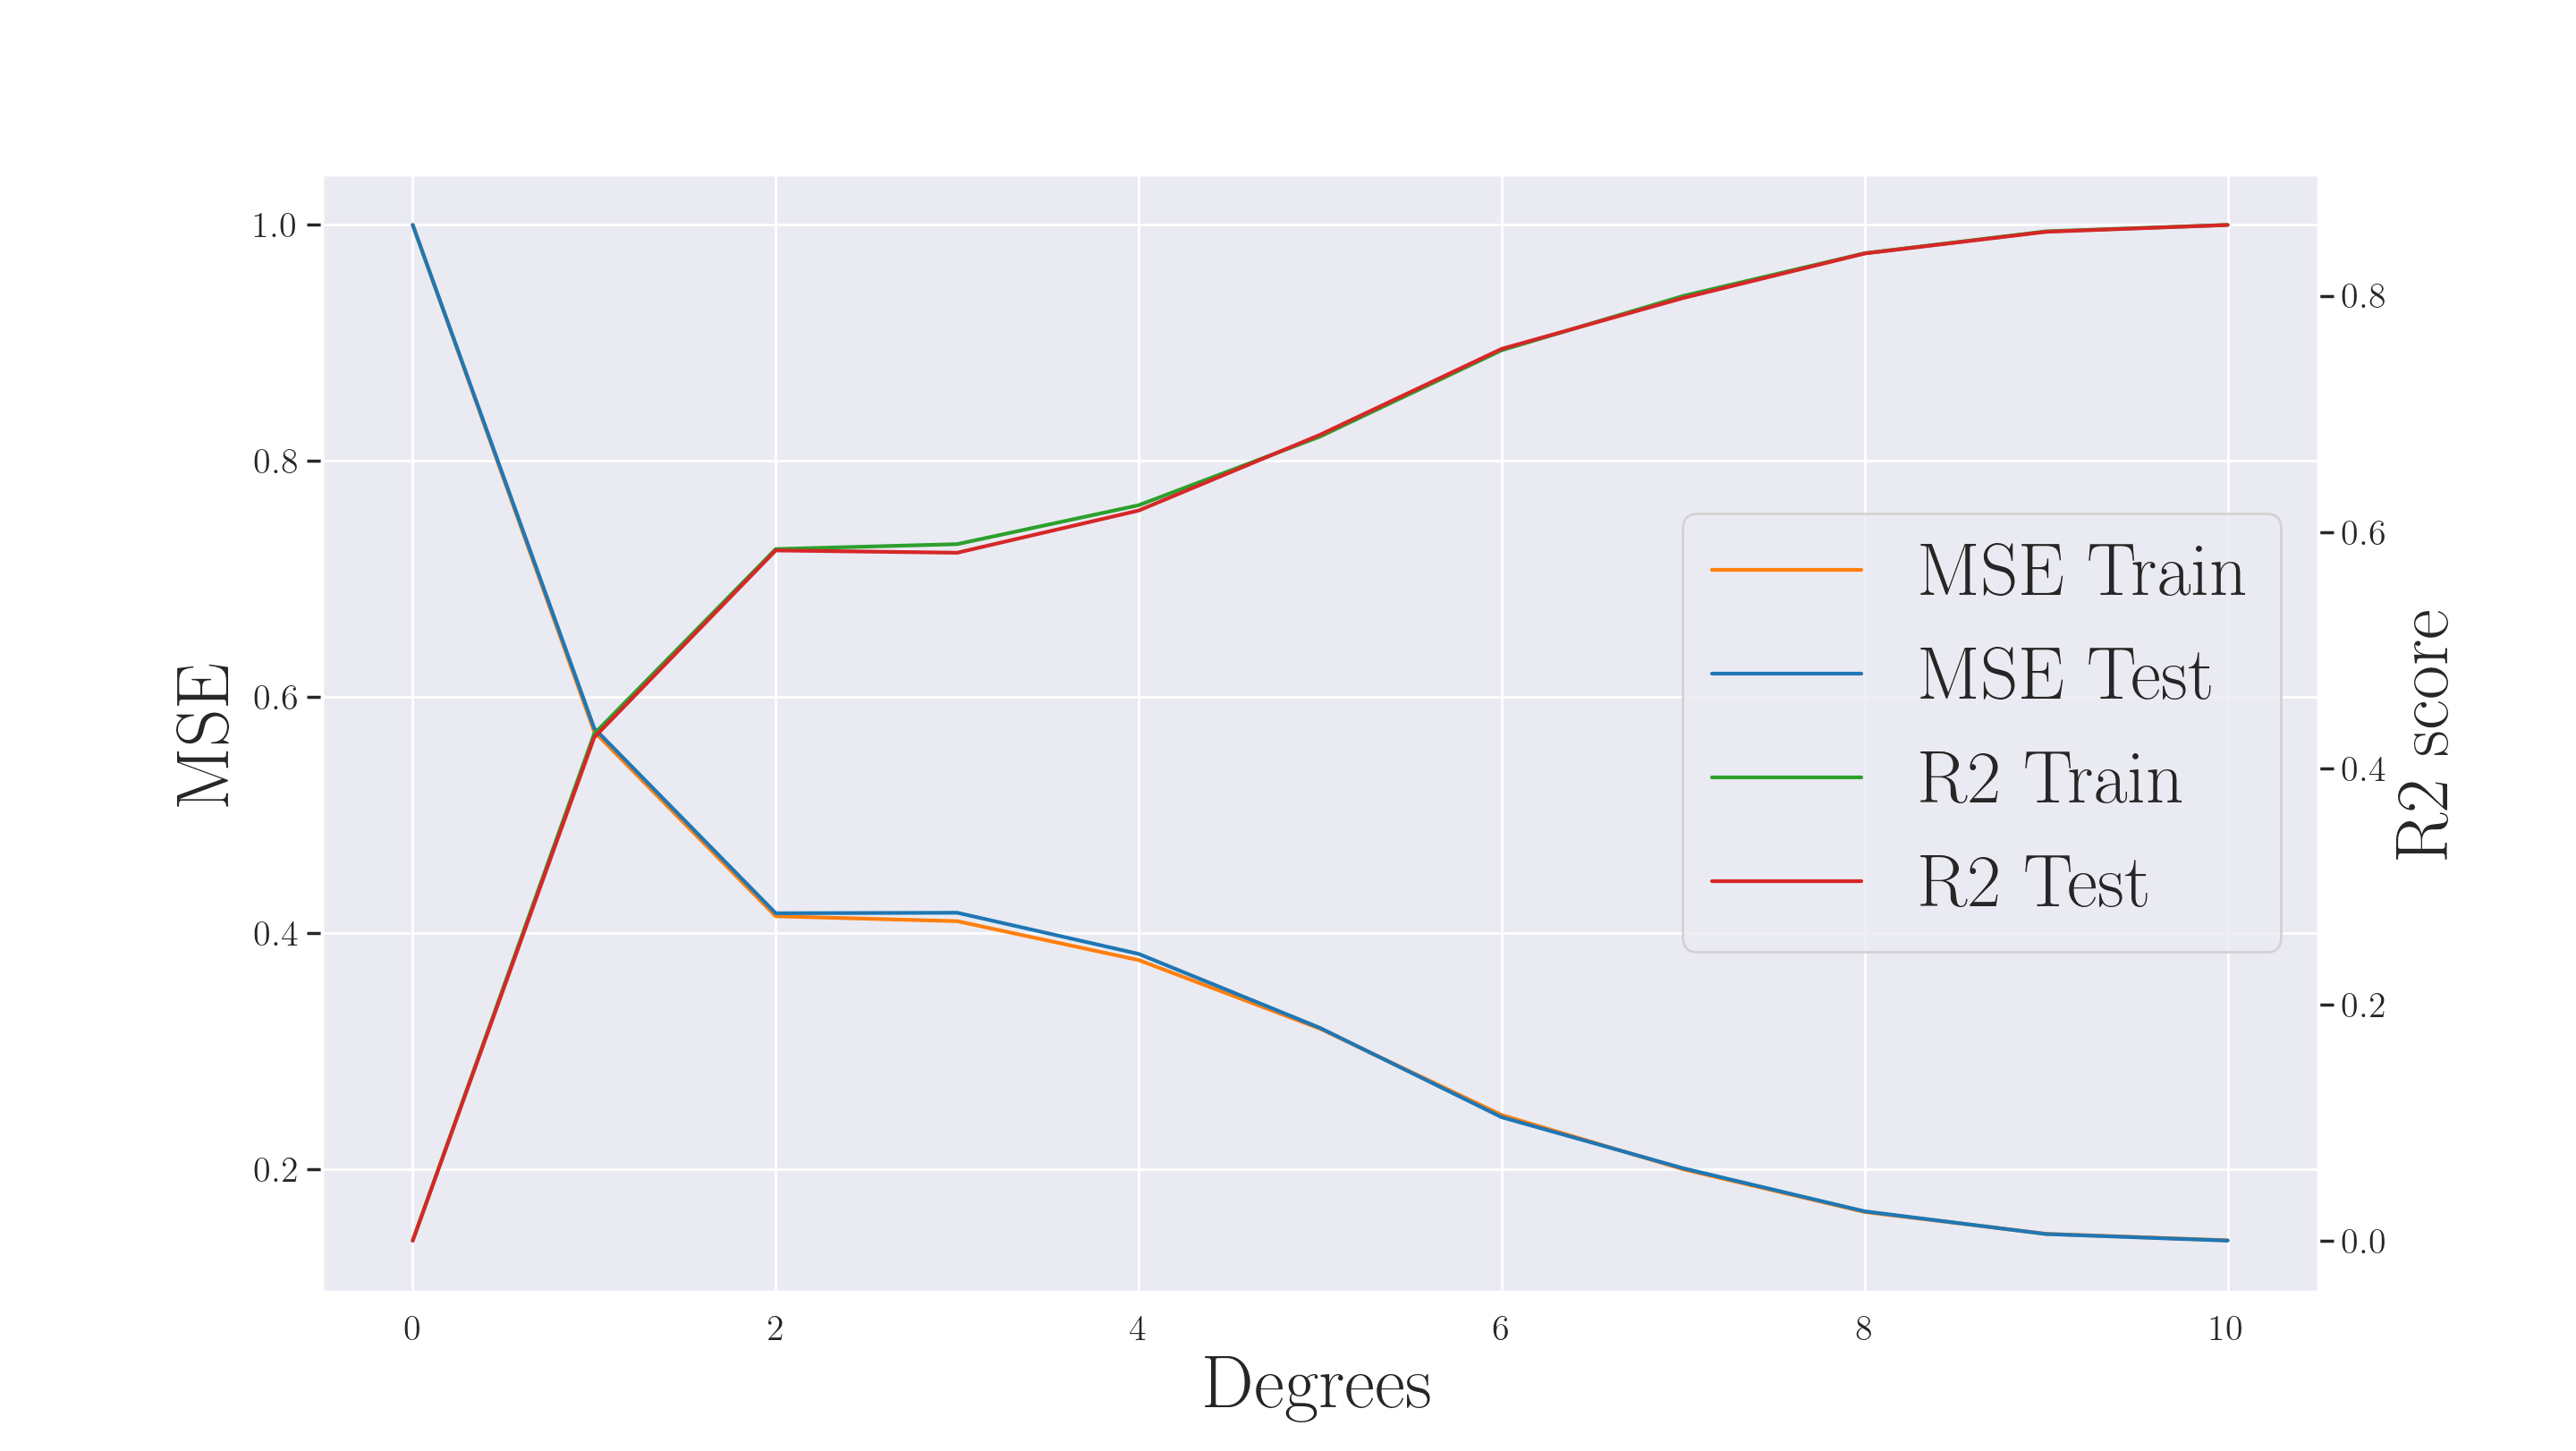
\includegraphics[width=\linewidth]{images/Figure_26.png}
	\caption{MSE and R2 score as a function of complexity with $\lambda = 10^{-5}$ for the terrain data modelled with Ridge regression. }
	\label{MSE Ridge terrain data}
\end{figure}
\noindent We then plotted the MSE for both OLS and Ridge with a lambda value of $10^{-5}$ in the same plot to see how these compered to each other. The plot is shown in figure \eqref{MSE OLS and Ridge}
\begin{figure}[H]
	\centering
	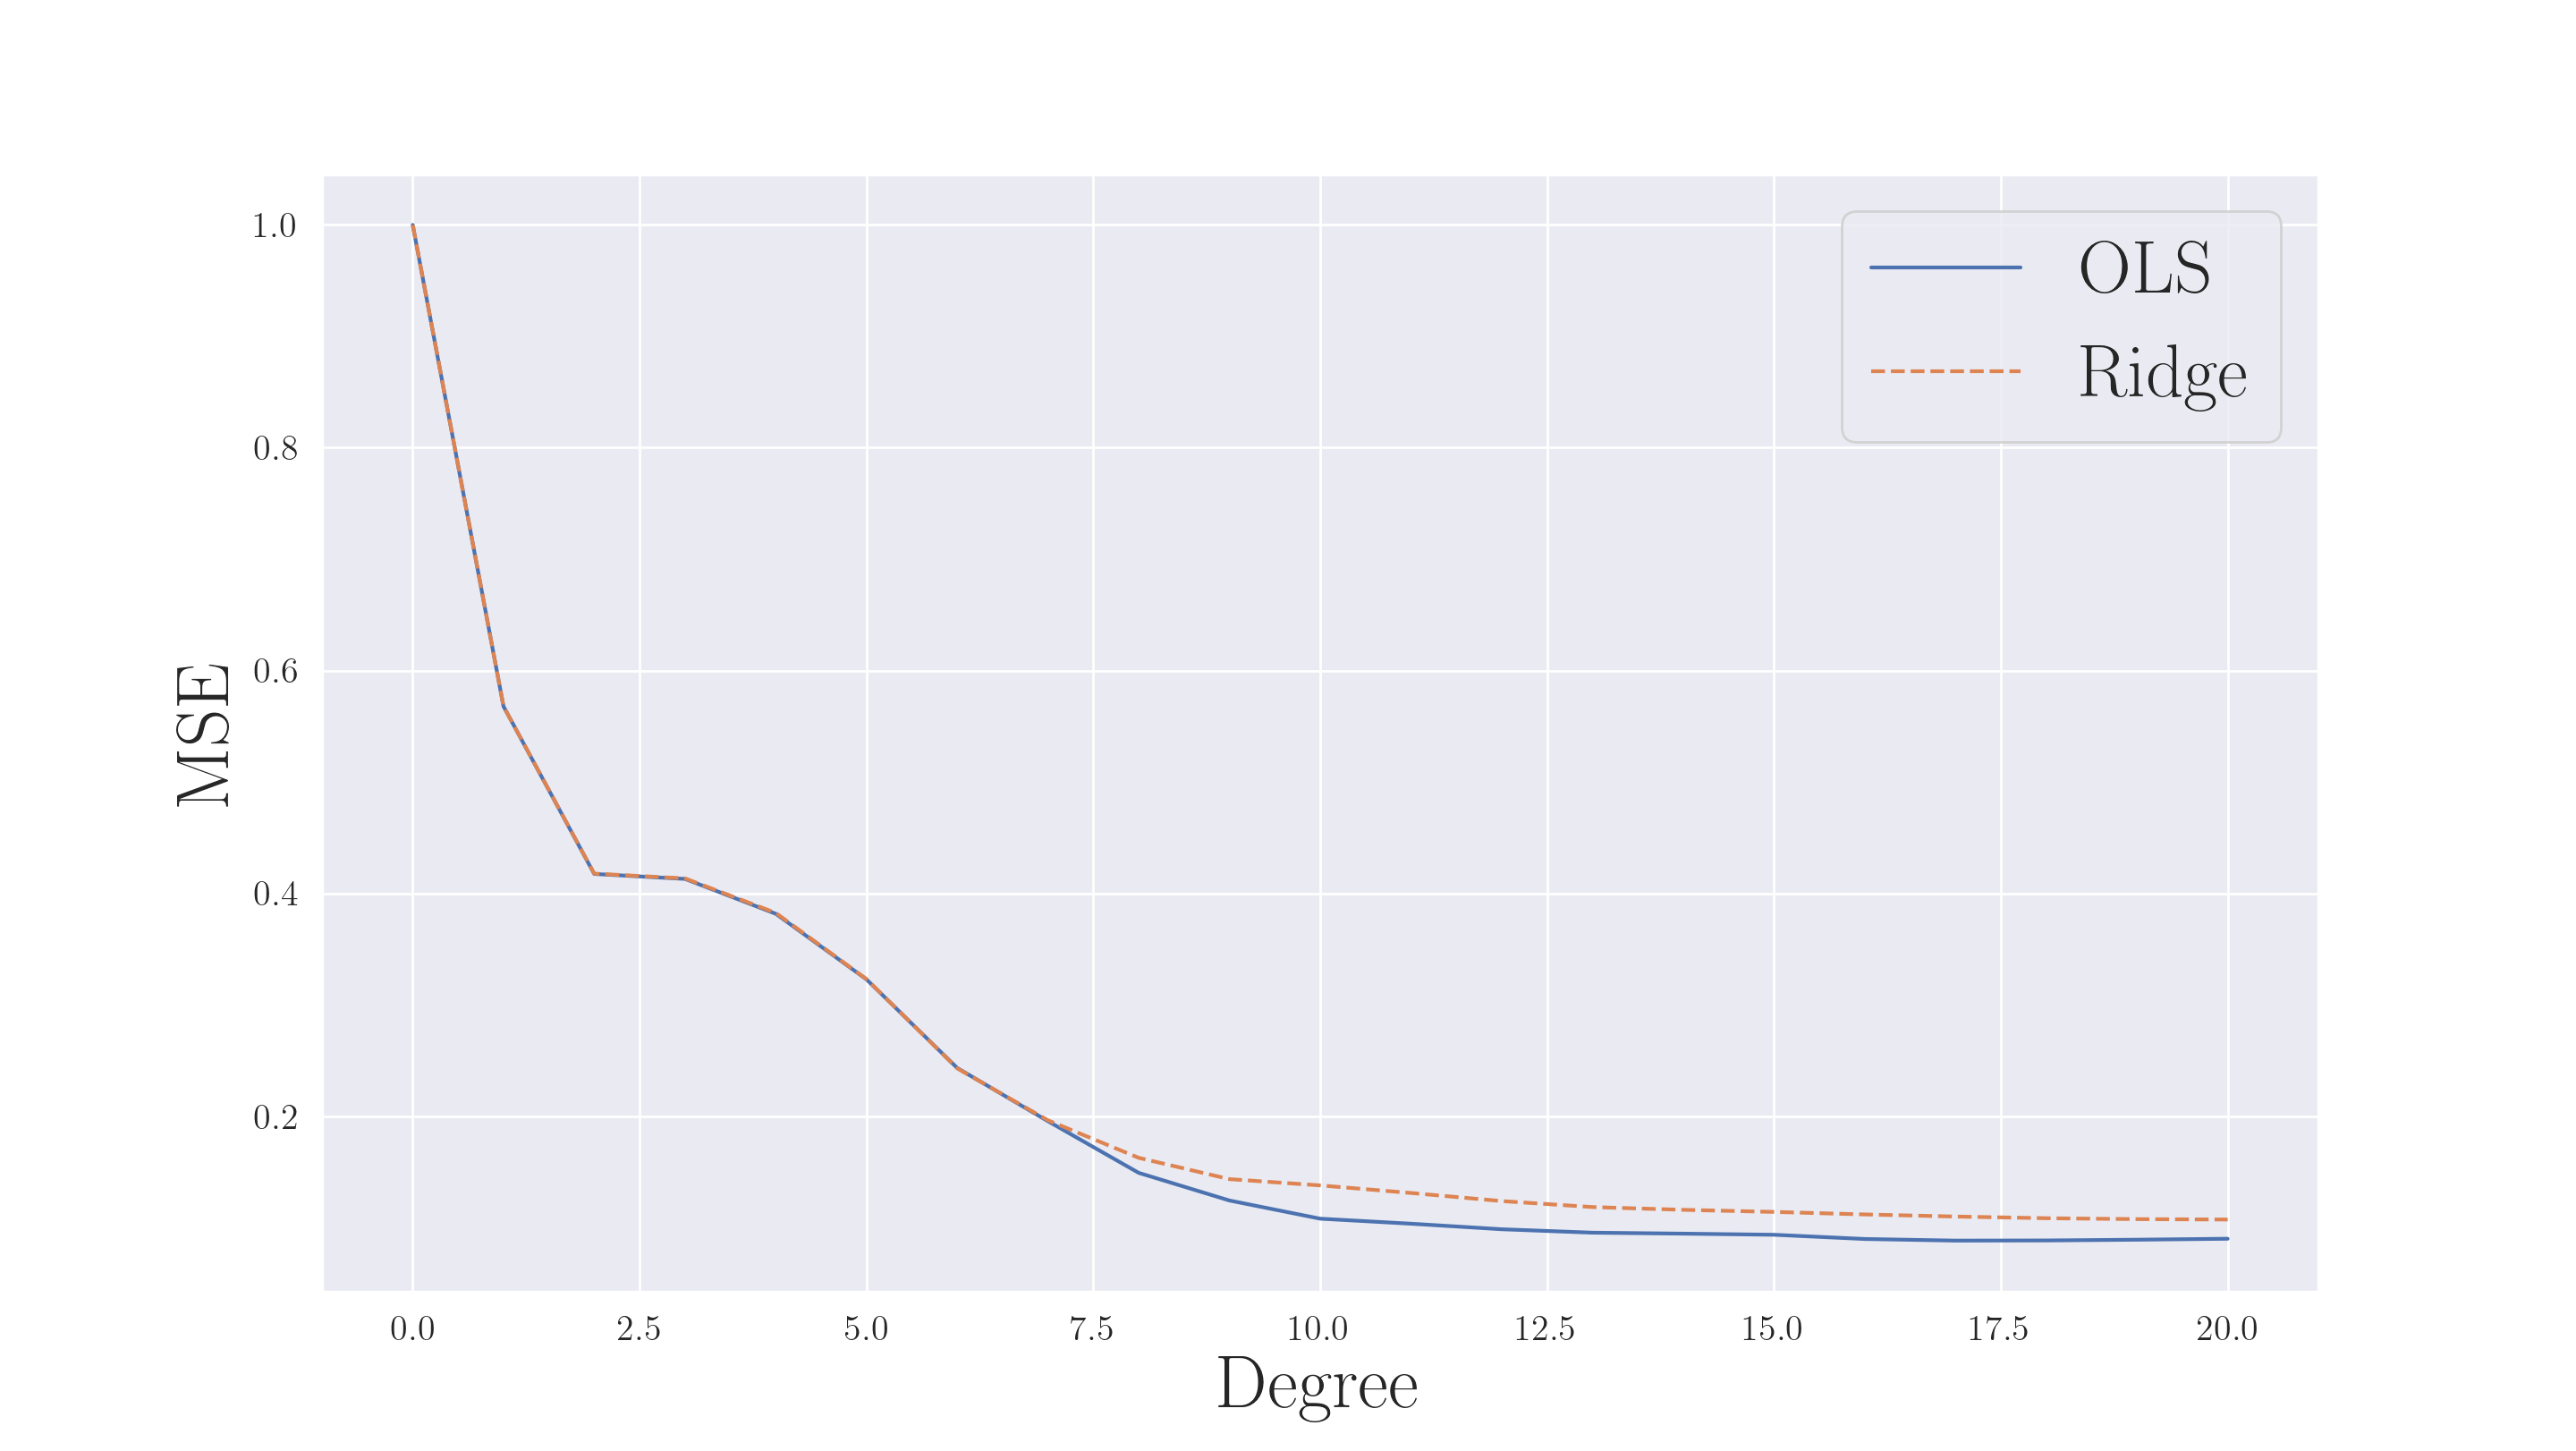
\includegraphics[width=\linewidth]{images/Figure_27.png}
	\caption{MSE as a function of complexity for both OLS and Ridge were Ridge is implemented with a $\lambda$ value of $10^{-5}$. }
	\label{MSE OLS and Ridge}
\end{figure}
%
\noindent The plot provided in figure \eqref{fig:cv_ridge_terrain} showcases the performance of Ridge Regression applied to real terrain data across various polynomial degrees and regularization strengths (denoted by $\lambda$).
%
\begin{figure}[H]
    \centering
    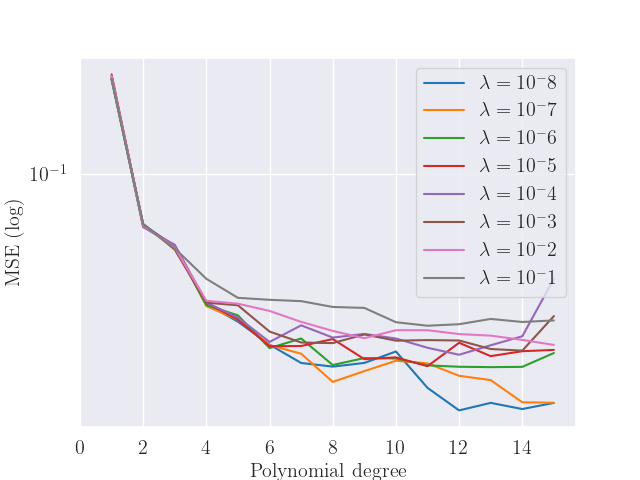
\includegraphics[width=\linewidth]{images/cv_ridge_terrain.png}
    \caption{MSE as a function of complexity for Ridge with terrain data, using cross validation with $k=5$.}
    \label{fig:cv_ridge_terrain}
\end{figure}

\subsubsection{LASSO}
\noindent Last we applied LASSO regression on the terrain data. Due to the time used to run this code the heat map is made out of 10 $\lambda$ values instead of 1000 as for Ridge. The heat map for both the training data and for test data is shown in figure \eqref{Heat map LASSO terrain training} and \eqref{Heat map LASSO terrain testing}. 
\begin{figure}[H]
	\centering
	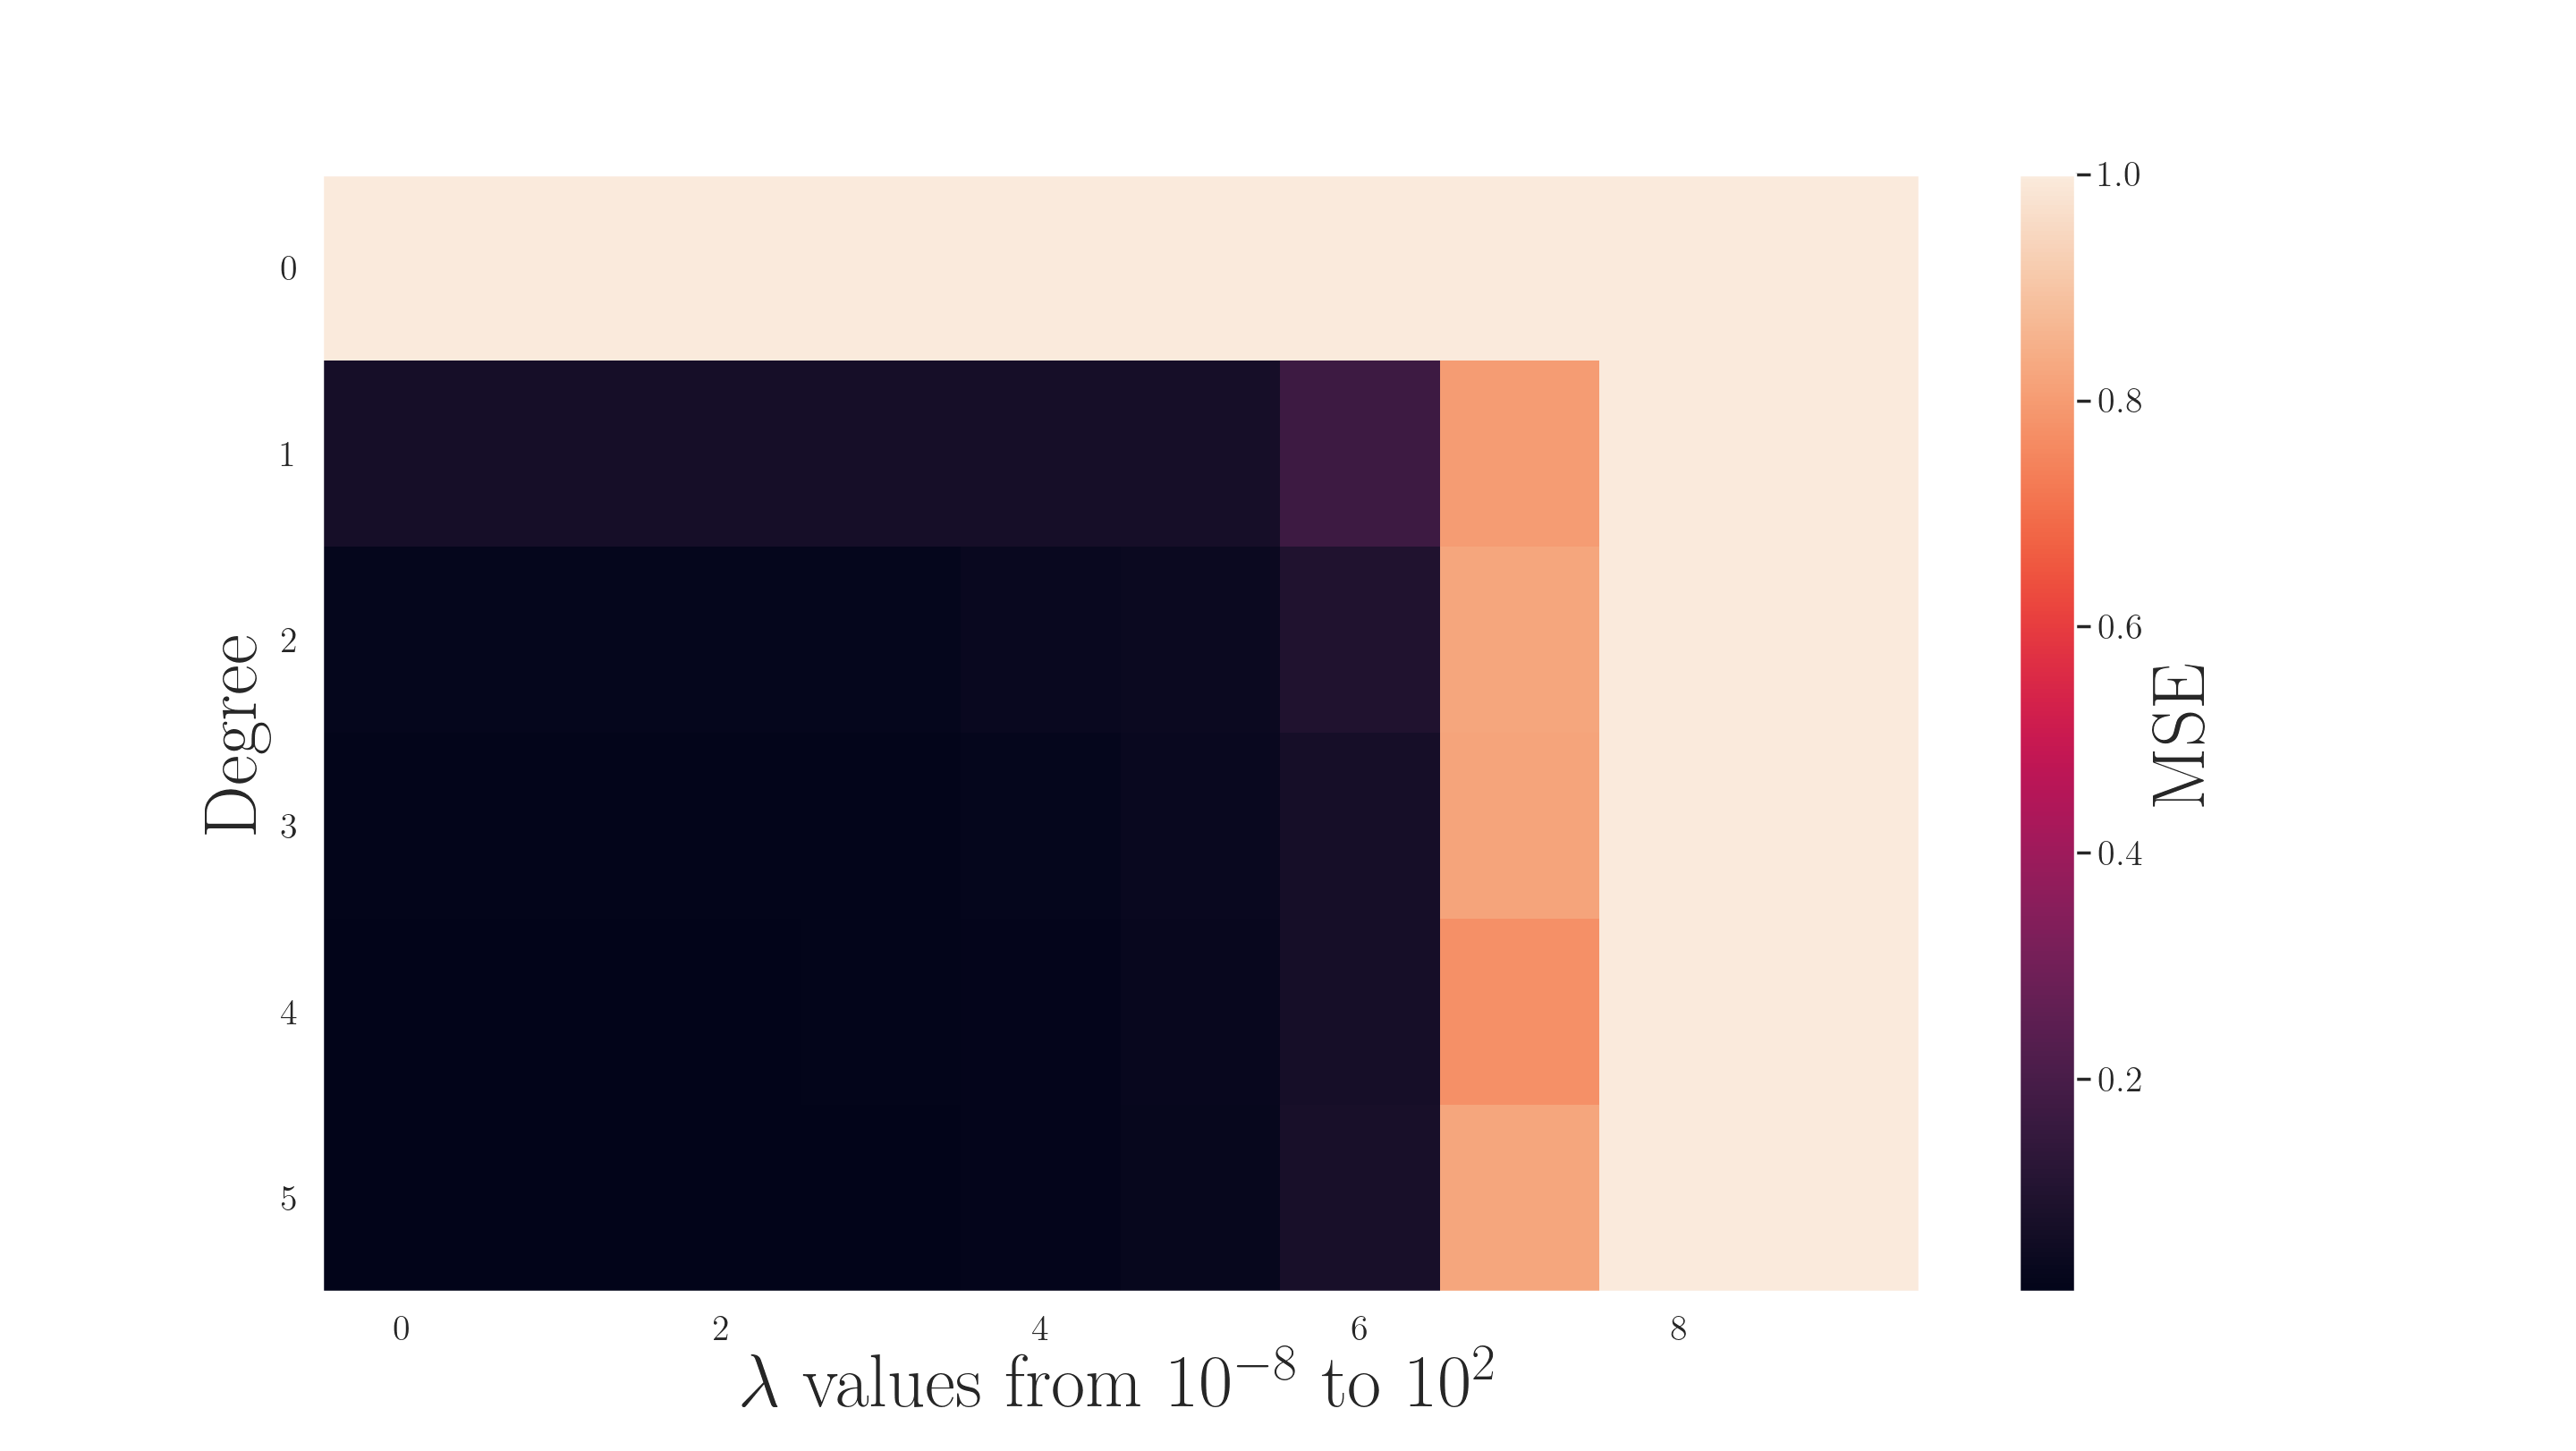
\includegraphics[width=\linewidth]{images/Figure_24.png}
	\caption{Heat map of the MSE for the training data, as a function of complexity and $lambda$ values for LASSO regression.}
	\label{Heat map LASSO terrain training}
\end{figure}
\begin{figure}[H]
	\centering
	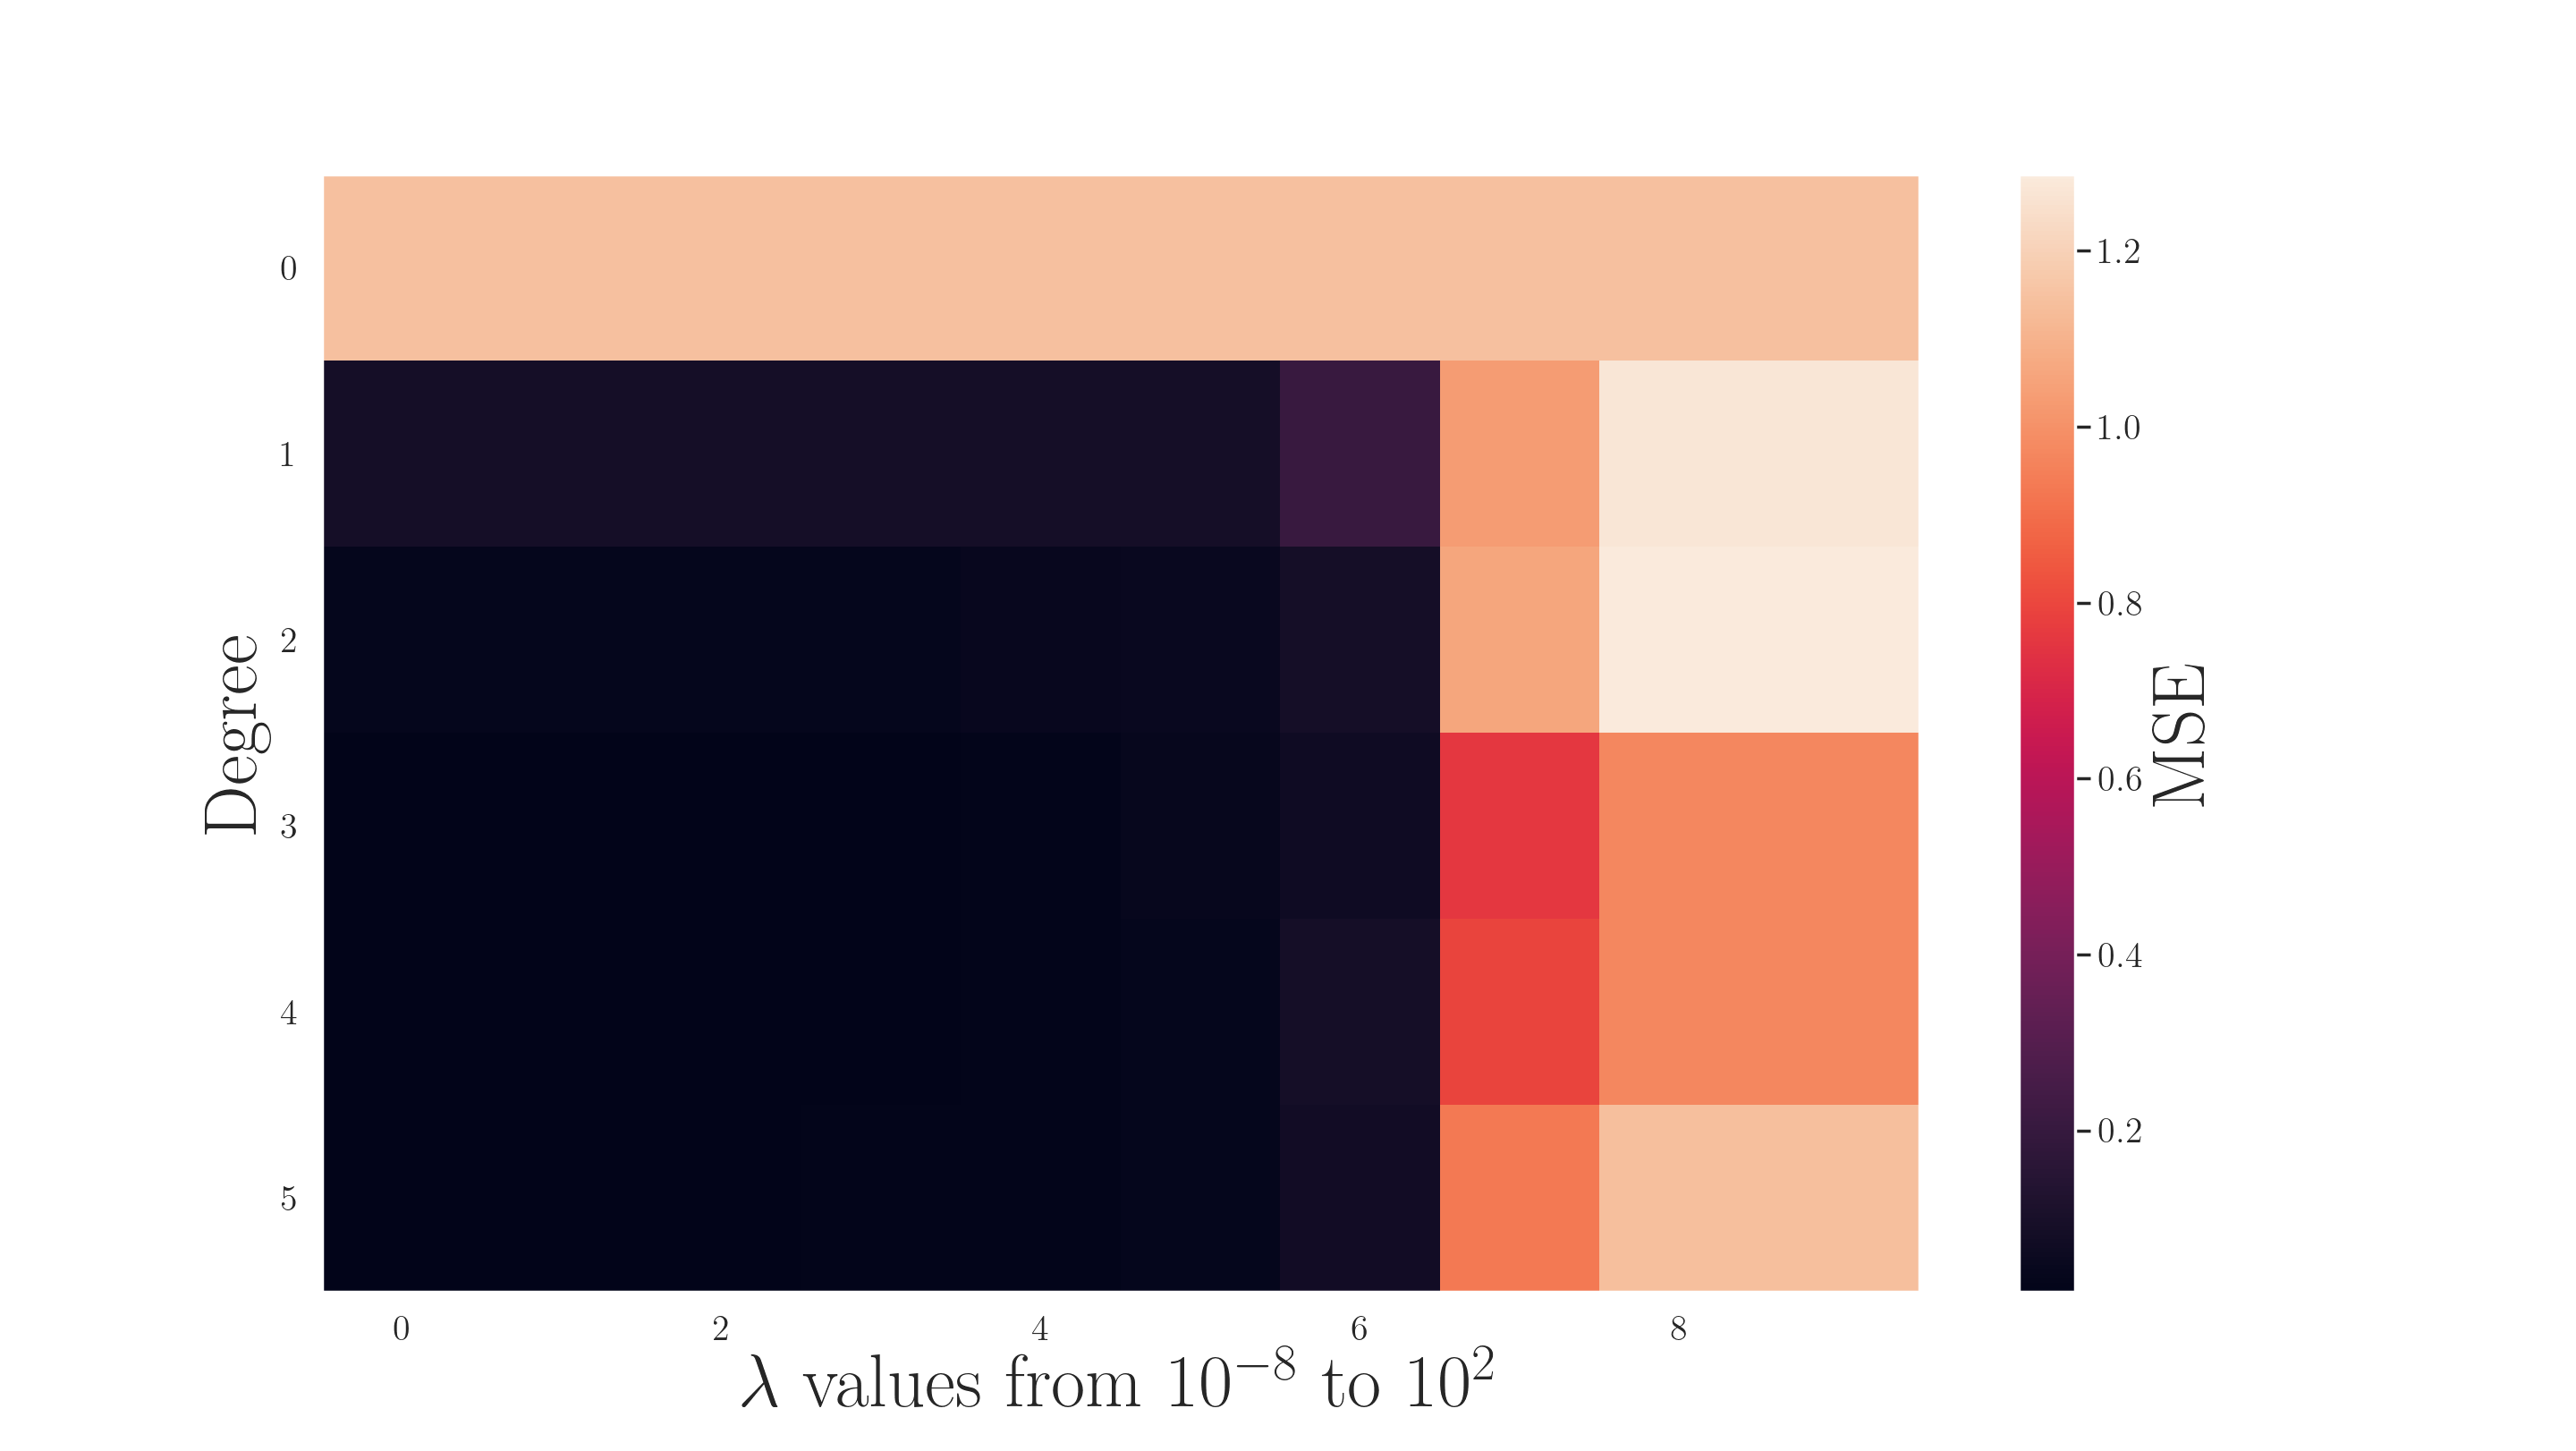
\includegraphics[width=\linewidth]{images/Figure_25.png}
	\caption{Heat map of the MSE for the test data, as a function of complexity and $lambda$ values for LASSO regression.}
	\label{Heat map LASSO terrain testing}
\end{figure}
%
\noindent We then also plotted the MSE and R2 score as a function of only complexity, where $\lambda$ was put to $\lambda = 10^{-5}$. The result are shown in figure \eqref{MSE LASSO terrain data}.
\begin{figure}[H]
	\centering
	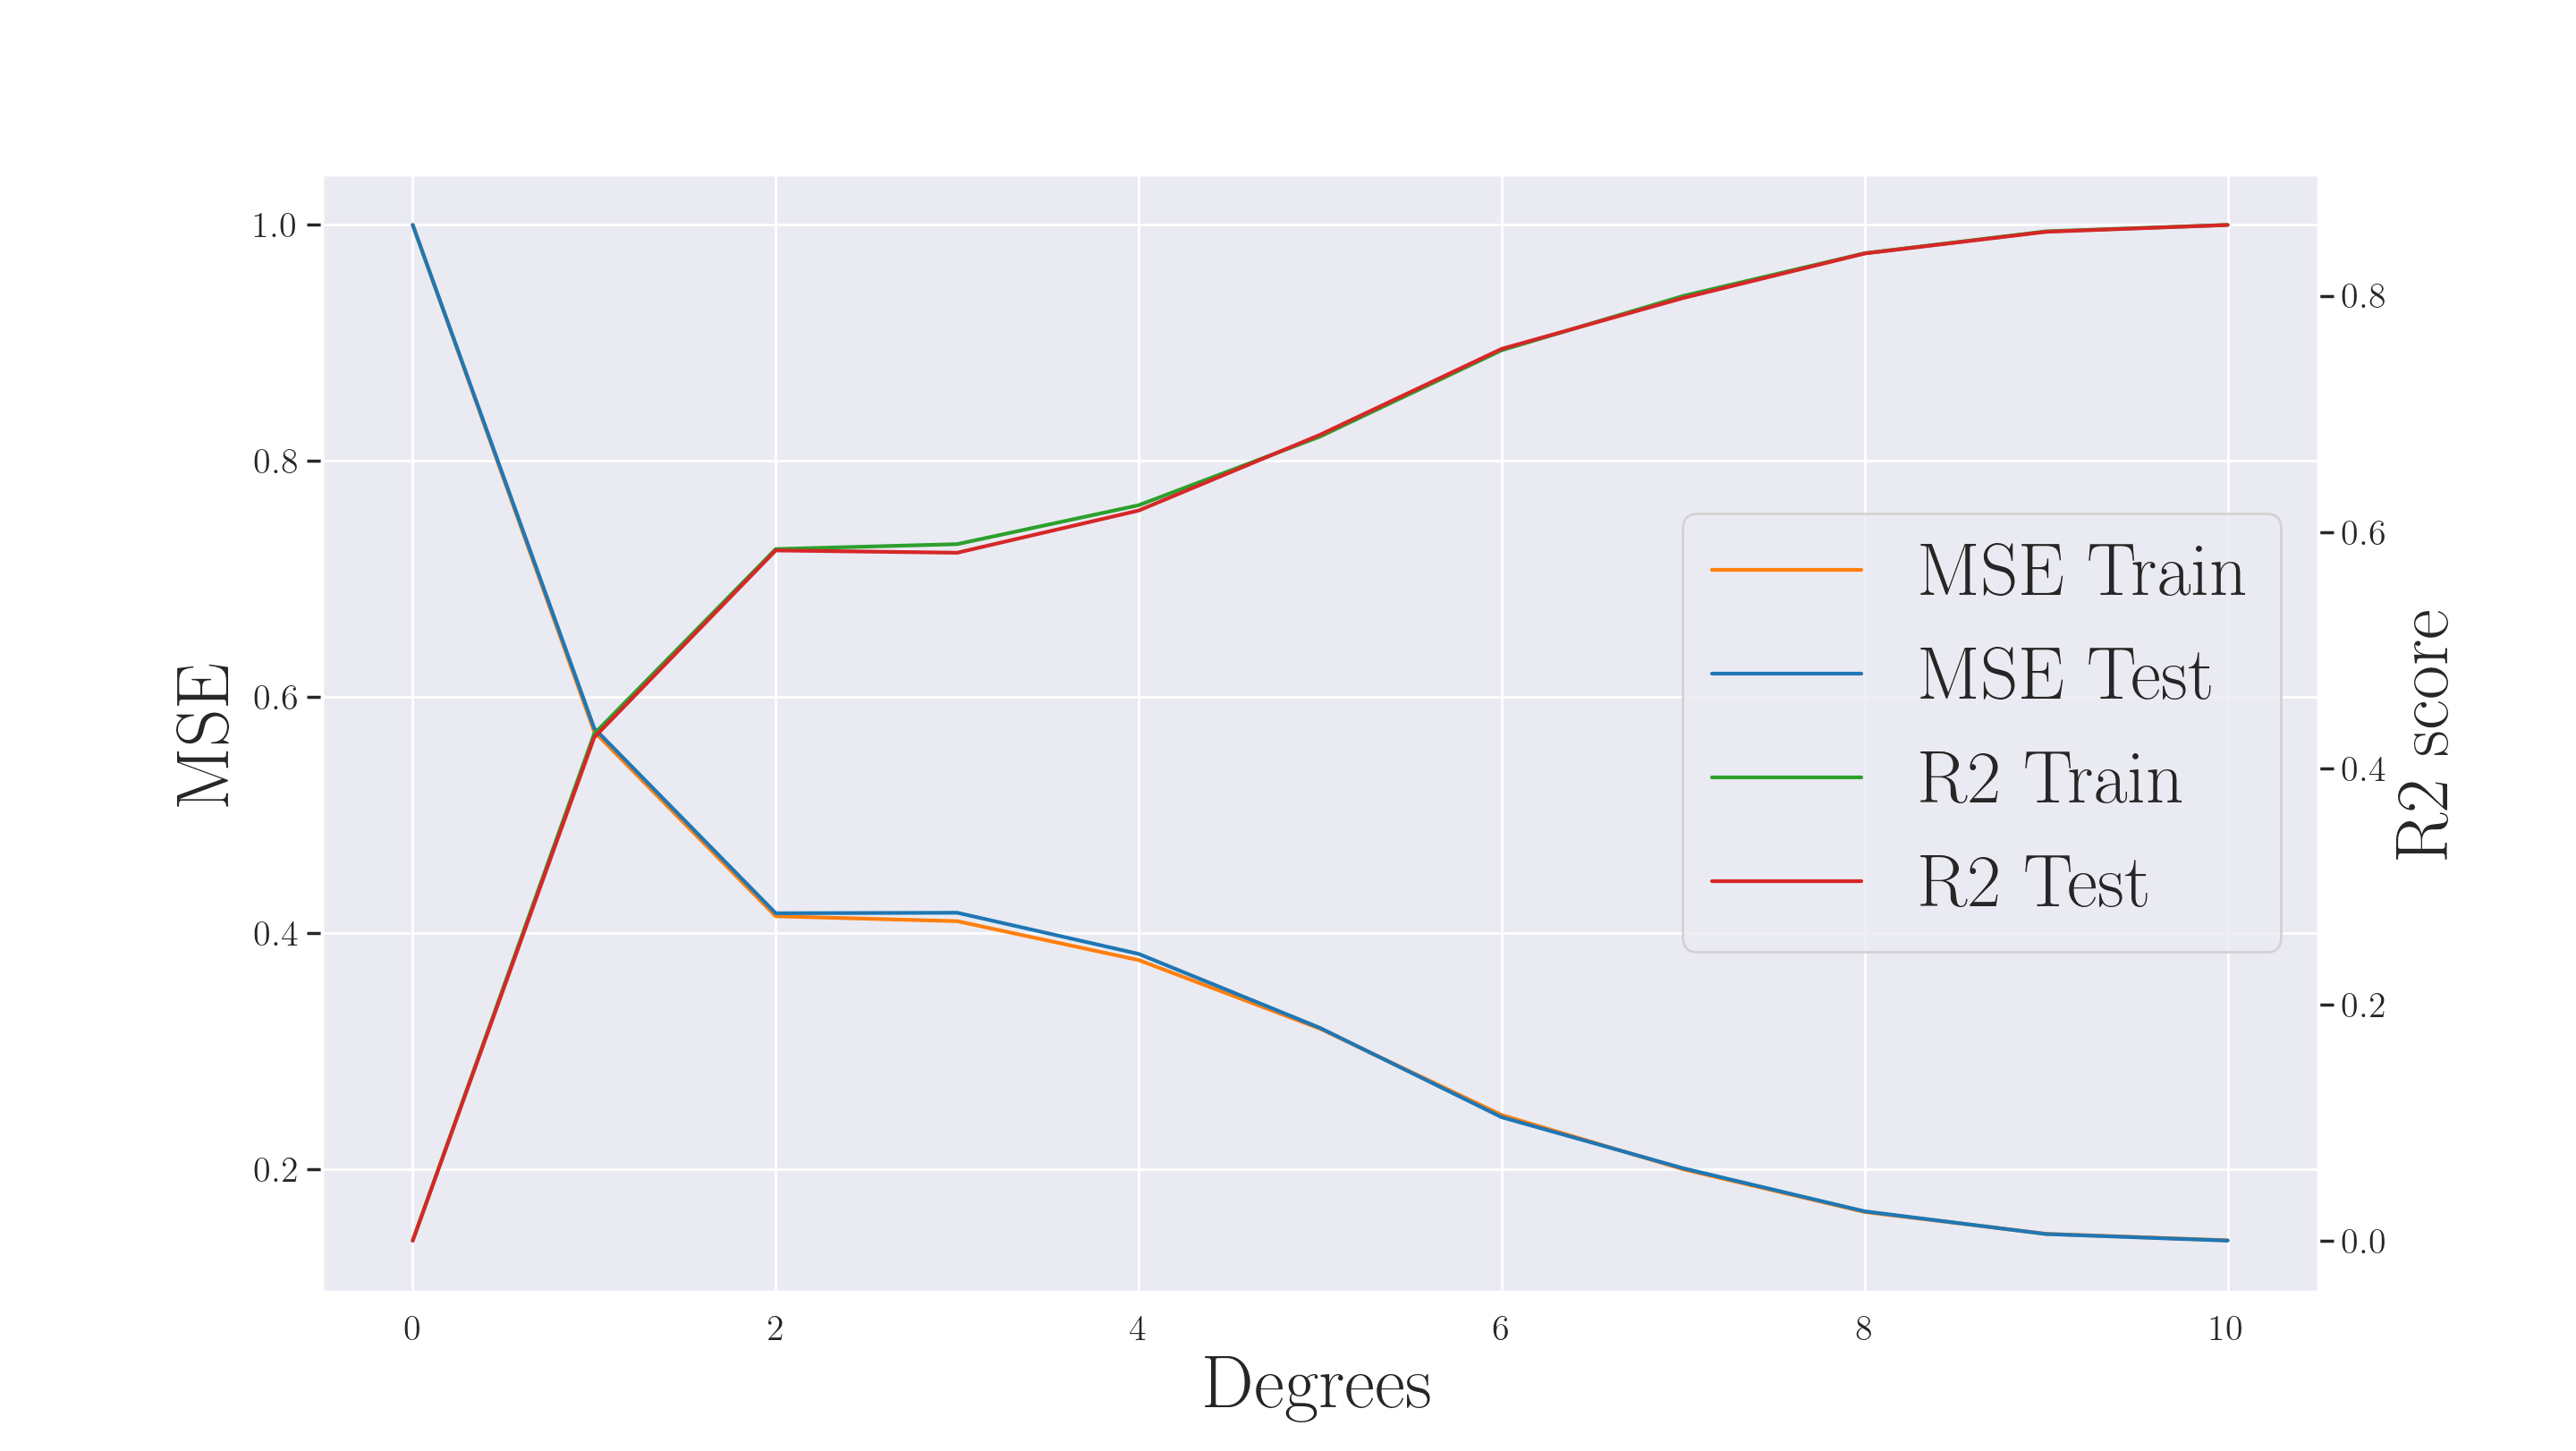
\includegraphics[width=\linewidth]{images/Figure_26.png}
	\caption{MSE and R2 score as a function of complexity with $\lambda = 10^{-5}$ for the terrain data modelled with LASSO regression. }
	\label{MSE LASSO terrain data}
\end{figure}
%
\noindent We then plotted the MSE as a function of complexity for both OLS, Ridge and LASSO to compere the three regression methods for the terrain data. The plot is shown in figure \eqref{MSE for OLS, Ridge and LASSO}.
\begin{figure}[H]
	\centering
	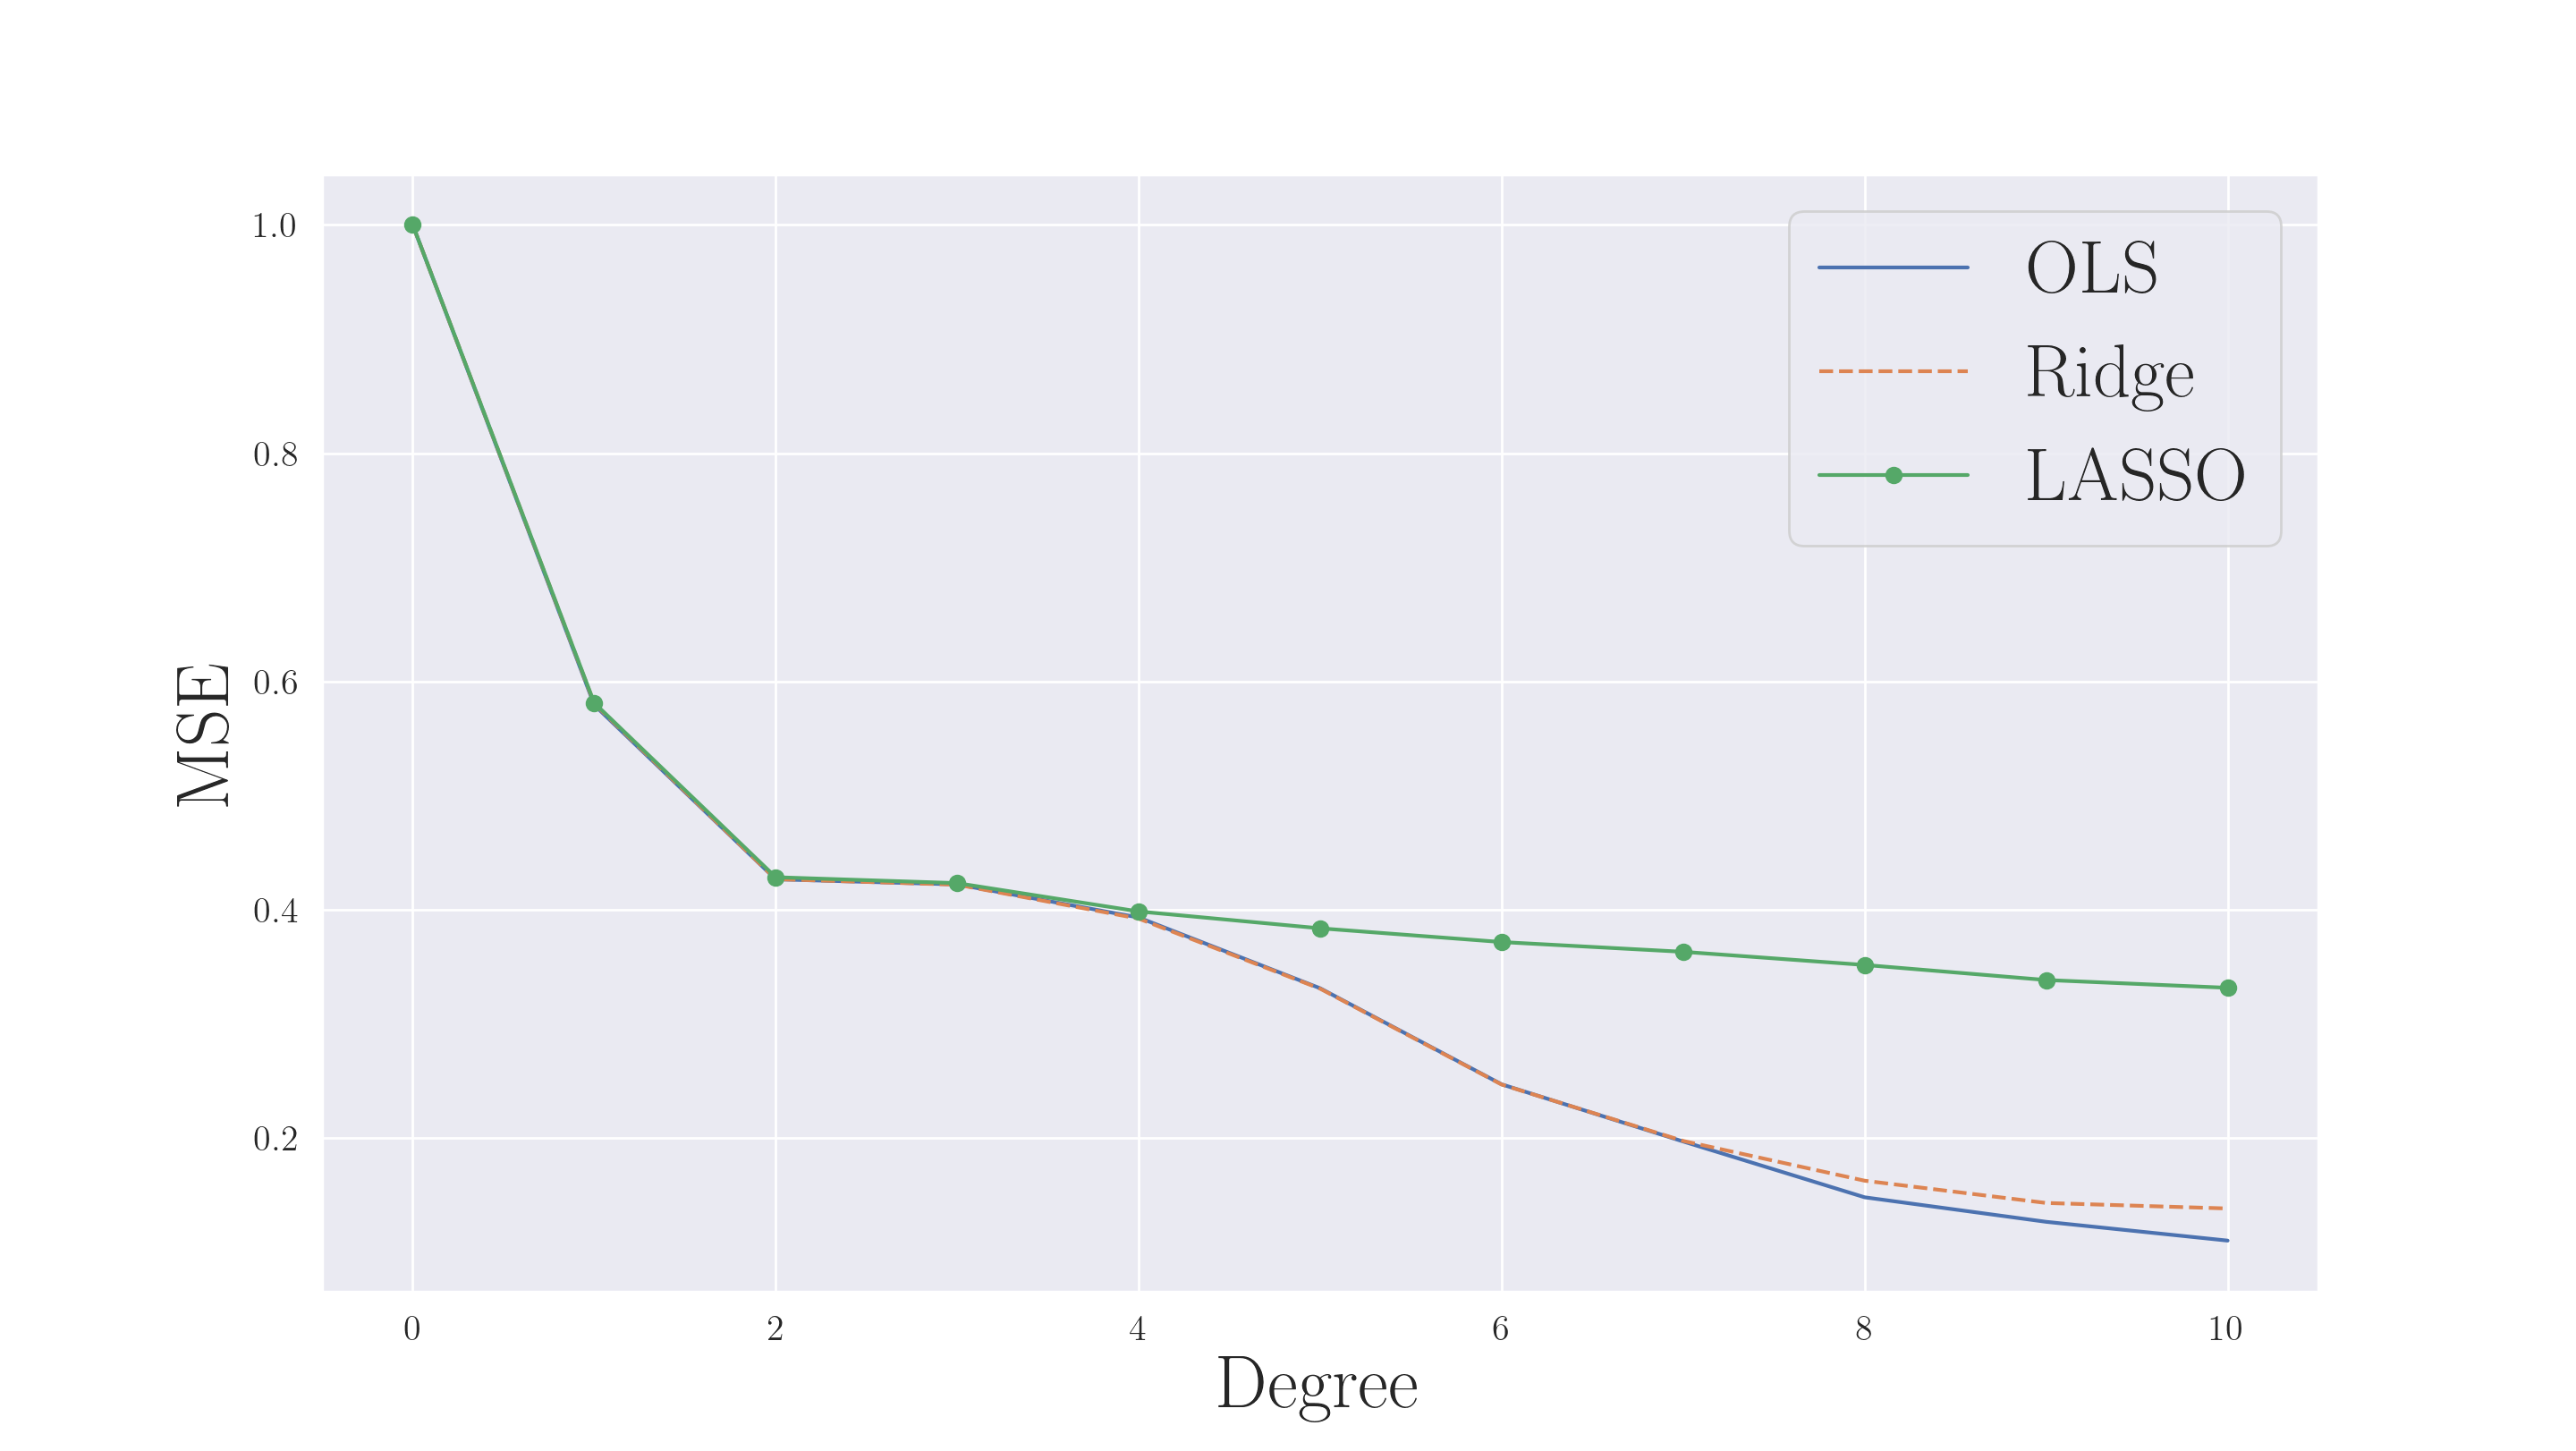
\includegraphics[width=\linewidth]{images/Figure_28.png}
	\caption{MSE as a function of complexity for both OLS, Ridge and LASSO were Ridge and LASSO are implemented with a $\lambda$ value of $10^{-5}$. }
	\label{MSE for OLS, Ridge and LASSO}
\end{figure}
%
\noindent Lastly the plotted in figure \eqref{fig:cv_lasso_terrain} showcases the performance of LASSO Regression applied to real terrain data across various polynomial degrees and regularization strengths (denoted by $\lambda$). 
%
\begin{figure}[H]
    \centering
    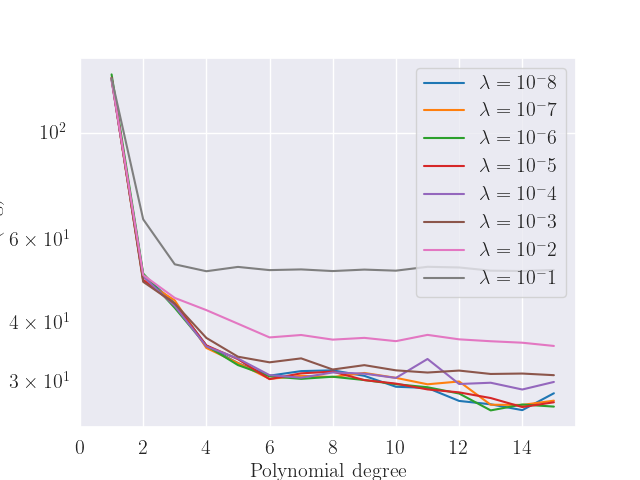
\includegraphics[width=\linewidth]{images/cv_lasso_real.png}
    \caption{MSE as a function of complexity for LASSO with terrain data, using cross validation with $k=5$.}
    \label{fig:cv_lasso_terrain}
\end{figure}
